\documentclass[a4paper,oneside,12pt]{report}
% Package yang diperlukan
\usepackage{fontspec}       % Font sistem untuk XeLaTeX/LuaLaTeX
\usepackage{setspace}       % Pengaturan jarak antarbaris
\usepackage{graphicx}      % Untuk memasukkan gambar
\usepackage{titling}       % Untuk kustomisasi halaman judul
\usepackage{geometry}      % Untuk mengatur margin halaman
\usepackage{listings}      % Untuk menampilkan blok kode
\usepackage{xcolor}        % Untuk menggunakan warna
\usepackage{float}         % Untuk kontrol penempatan float (seperti gambar)
\usepackage{hyperref}      % Untuk membuat hyperlink (URL, referensi)
\usepackage{indentfirst}   % Untuk memberi indentasi pada paragraf pertama setiap seksi
\usepackage{url}           % Untuk format URL
\usepackage{xurl}          % Untuk pemutusan tautan URL yang lebih baik
\usepackage{fancyhdr}      % Untuk kustomisasi header dan footer
\usepackage{tocloft}       % Untuk kustomisasi Daftar Isi
\usepackage{bookmark}      % Untuk manajemen bookmark PDF yang lebih baik
\usepackage{amsmath}       % Untuk rumus matematika
\usepackage{amssymb}       % Untuk simbol matematika
\usepackage{booktabs}      % Untuk tabel yang lebih rapi
\usepackage{caption}
\usepackage{subcaption}    % Untuk tata letak gambar berdampingan
\usepackage{tabularx}      % Untuk tabel dengan lebar otomatis sesuai margin
\usepackage{array}         % Untuk kontrol kolom tabel
\usepackage{enumitem}      % Untuk kontrol kerapatan daftar
\usepackage[none]{hyphenat} % Nonaktifkan seluruh pemotongan kata bertanda hubung
\usepackage{microtype}     % Tipografi halus dan protrusion antislop

% Font dan spasi standar laporan praktikum
\setmainfont{Times New Roman}
\onehalfspacing

%======================================================================
% PENGATURAN GEOMETRI HALAMAN
%======================================================================
\geometry{left=3cm, right=2.5cm, top=2cm, bottom=2.5cm}
\sloppy
\tolerance=10000
\emergencystretch=3em
\hfuzz=1.5pt
\hbadness=10000
\hyphenpenalty=10000
\exhyphenpenalty=10000
\righthyphenmin=62
\lefthyphenmin=62

%======================================================================
% PENGATURAN WARNA UNTUK BLOK KODE
%======================================================================
\definecolor{codegreen}{rgb}{0,0.6,0}
\definecolor{codegray}{rgb}{0.5,0.5,0.5}
\definecolor{codepurple}{rgb}{0.58,0,0.82}
\definecolor{backcolour}{rgb}{0.95,0.95,0.92}
\definecolor{darkblue}{rgb}{0,0,0.6}

%======================================================================
% PENGATURAN BLOK KODE (LISTINGS)
%======================================================================
\lstdefinestyle{commonstyle}{
    backgroundcolor=\color{backcolour},
    breakatwhitespace=false,
    breaklines=true,
    captionpos=b,
    keepspaces=true,
    numbers=left,
    numbersep=5pt,
    showspaces=false,
    showstringspaces=false,
    showtabs=false,
    tabsize=2,
    frame=single,
    basicstyle=\ttfamily\footnotesize,
    numberstyle=\tiny\color{codegray},
    columns=flexible,
    postbreak=\mbox{\textcolor{red}{$\hookrightarrow$}\space},
    breakindent=0pt,
    breakautoindent=false
}
\lstdefinestyle{pythonstyle}{
    style=commonstyle,
    language=Python,
    commentstyle=\color{codegreen},
    keywordstyle=\color{darkblue},
    stringstyle=\color{codepurple},
    emph={import,from,class,def,for,while,if,else,elif,try,except,finally},
    emphstyle=\color{darkblue}
}

%======================================================================
% PENGATURAN LAIN-LAIN
%======================================================================
\newcommand{\customfbox}[1]{%
  \setlength{\fboxsep}{0pt}%
  \setlength{\fboxrule}{0.5pt}%
  \fcolorbox{black}{white}{#1}%
}
\renewcommand{\figurename}{Gambar}
\renewcommand{\thefigure}{\arabic{figure}}
\renewcommand{\tablename}{Tabel}
\renewcommand{\thetable}{\arabic{table}}
\renewcommand{\theequation}{\arabic{equation}}
\counterwithout{figure}{chapter}
\counterwithout{table}{chapter}
\counterwithout{equation}{chapter}
\hypersetup{
    colorlinks=true,
    linkcolor=black,
    filecolor=black,
    urlcolor=black,
    citecolor=black,
    pdftitle={Laporan Praktikum Penambangan Data Pertemuan 6},
    pdfpagemode=FullScreen,
    breaklinks=true
}
\pagestyle{fancy}
\fancyhf{}
\fancyfoot[C]{\thepage}
\renewcommand{\headrulewidth}{0pt}
\fancypagestyle{plain}{
    \fancyhf{}
    \fancyfoot[C]{\thepage}
    \renewcommand{\headrulewidth}{0pt}
}
\renewcommand{\contentsname}{Daftar Isi}
\renewcommand{\bibname}{Daftar Pustaka}
\renewcommand{\thechapter}{}
\renewcommand{\chaptername}{}
\renewcommand{\thesection}{\arabic{chapter}.\arabic{section}}
\renewcommand{\thesubsection}{\thesection.\arabic{subsection}}
\setcounter{secnumdepth}{3}
\setcounter{tocdepth}{3}
\renewcommand{\cftchapdotsep}{\cftdotsep}
\renewcommand{\cftchapleader}{\cftdotfill{\cftchapdotsep}}
\setlength{\cftchapindent}{0em}
\setlength{\cftsecindent}{2em}
\setlength{\cftsubsecindent}{4em}
\setlength{\cftchapnumwidth}{0em}
\setlength{\cftsecnumwidth}{2.5em}
\setlength{\cftsubsecnumwidth}{3.2em}
\setlength{\cftbeforechapskip}{4pt}
\setlength{\cftbeforesecskip}{1.5pt}
\setlength{\cftbeforesubsecskip}{0.5pt}
\renewcommand{\cftchappresnum}{}
\renewcommand{\cftchapaftersnum}{}
\newcommand{\tocboldsection}[1]{%
  \protect\renewcommand{\protect\cftchapfont}{\protect\bfseries}%
  #1%
  \protect\renewcommand{\protect\cftchapfont}{}%
}

%======================================================================
% AWAL DOKUMEN
%======================================================================
\begin{document}

% Halaman Judul
\newgeometry{left=3cm, right=2.5cm, top=2.5cm, bottom=3cm}
\begin{titlingpage}
\begin{spacing}{1}
\begin{center}
\vspace*{0.2cm}
{\large \textbf{\MakeUppercase{Laporan Praktikum}}} \\[0.4cm]
{\large \textbf{\MakeUppercase{Praktikum Penambangan Data}}} \\[0.4cm]
{\large \textbf{\MakeUppercase{Pertemuan 6}}} \\[0.4cm]
{\large \textbf{\MakeUppercase{Clustering dan Association Rule}}} \\[1.5cm]


\includegraphics[height=7cm]{images/UGM.png} \\[0.7cm]

{\normalsize \textbf{Disusun oleh:}} \\[0.4cm]
\begin{tabular}{@{}l l @{}}
  \textbf{Nama}           & : Hafidz Rizqullah Prasetya \\
  \textbf{NIM}            & : 24/535493/SV/24243 \\
  \textbf{Kelas}          & : PL5A1 \\
  \textbf{Dosen Pengampu} & : Dr. Imam Fahrurrozi, S.T., M.Cs.
\end{tabular} \\[1.2cm]

{\normalsize \textbf{PROGRAM STUDI D-IV}} \\[0.2cm]
{\normalsize \textbf{TEKNOLOGI REKAYASA PERANGKAT LUNAK}} \\[0.2cm]
{\normalsize \textbf{DEPARTEMEN TEKNIK ELEKTRO DAN INFORMATIKA}} \\[0.2cm]
{\normalsize \textbf{SEKOLAH VOKASI}} \\[0.2cm]
{\normalsize \textbf{UNIVERSITAS GADJAH MADA}} \\[0.2cm]
{\normalsize \textbf{YOGYAKARTA}} \\[0.2cm]
{\normalsize \textbf{2026}} \\[1.2cm]
\end{center}
\end{spacing}
\end{titlingpage}
\restoregeometry

\thispagestyle{empty}
\clearpage
\stepcounter{page}
\thispagestyle{empty}

% --- Daftar Isi ---
\addcontentsline{toc}{chapter}{Daftar Isi}
\begin{spacing}{0.92}
\tableofcontents
\end{spacing}
\clearpage

% Mengatur penomoran halaman menjadi arab dan mulai dari 3
\pagenumbering{arabic}
\setcounter{page}{3}

\chapter[Tujuan Praktikum]{Tujuan Praktikum}
Berdasarkan Modul Pertemuan 6 Praktikum Penambangan Data, tujuan praktikum ini adalah:
\begin{enumerate}[noitemsep, topsep=4pt, parsep=2pt]
   \item Mahasiswa memahami konsep dasar unsupervised learning dan perbedaannya dengan supervised learning.
   \item Mahasiswa memahami prinsip kerja, kelebihan, dan kelemahan algoritma klasterisasi K-Means, K-Medoids (Partitioning Around Medoids / PAM), dan DBSCAN (Density-Based Spatial Clustering of Applications with Noise).
   \item Mahasiswa dapat mengevaluasi kualitas klaster memakai metrik evaluasi internal seperti Inertia (Within-Cluster Sum of Squares / WCSS) dan Silhouette Score, serta menentukan jumlah klaster optimal ($K$) memakai Elbow Method dan KneeLocator.
   \item Mahasiswa dapat menerapkan visualisasi hasil klasterisasi dalam dimensi dua memakai Matplotlib dan Seaborn, serta dimensi tiga memakai Plotly Express.
   \item Mahasiswa mampu melakukan analisis profil klaster (cluster profiling) dan interpretasi bisnis atas segmen nasabah yang terbentuk.
   \item Mahasiswa memahami konsep dasar Association Rule Mining, metrik evaluasi Support, Confidence, dan Lift, prinsip Apriori (anti-monotonicity of support), serta mekanisme pemangkasan kandidat itemset (lattice pruning).
\end{enumerate}

\clearpage

\chapter{Dasar Teori}

\section{Unsupervised Learning}
Unsupervised learning adalah paradigma pembelajaran mesin yang melatih model pada data tanpa label target ($y$). Model bertugas mengenali pola keteraturan, kesamaan atribut, atau struktur kepadatan yang terbentuk secara alami dari matriks fitur masukan ($X$) \cite{retnoningsih2020,santoso2021}. Gambar~\ref{fig:sup-unsup} memperlihatkan perbedaan konsep kedua paradigma ini.

\begin{figure}[H]
\centering
\fbox{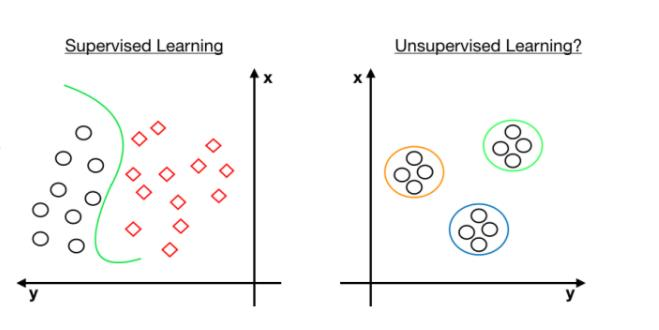
\includegraphics[width=0.72\textwidth]{images/gambar-6-2-1-supervised-vs-unsupervised.png}}
\caption{Perbandingan pembelajaran mesin: supervised learning memakai data berlabel sebagai acuan target, sedangkan unsupervised learning mengelompokkan data tanpa label \cite{tan2019}.}
\label{fig:sup-unsup}
\end{figure}

Perbedaan pokok kedua pendekatan ini meliputi:
\begin{itemize}
    \item \textbf{Supervised Learning:} Memetakan hubungan fungsi matematis $f(X) \approx y$ antara pasangan masukan dan target yang telah diketahui. Tujuannya adalah memprediksi nilai target pada sampel baru melalui tugas klasifikasi atau regresi.
    \item \textbf{Unsupervised Learning:} Hanya menerima variabel fitur masukan $X$. Tujuannya adalah mengidentifikasi struktur intrinsik data, seperti pengelompokan (clustering), penemuan aturan asosiasi (association rules), atau reduksi dimensi data.
\end{itemize}

Penerapan unsupervised learning di industri mencakup segmentasi pelanggan untuk mengelompokkan nasabah berdasarkan pola transaksi, deteksi anomali untuk mendeteksi transaksi kartu kredit mencurigakan, serta sistem rekomendasi berbasis kesamaan preferensi pengguna \cite{han2011}. Contoh segmentasi nasabah ditunjukkan pada Gambar~\ref{fig:customer-seg}.

\begin{figure}[H]
\centering
\fbox{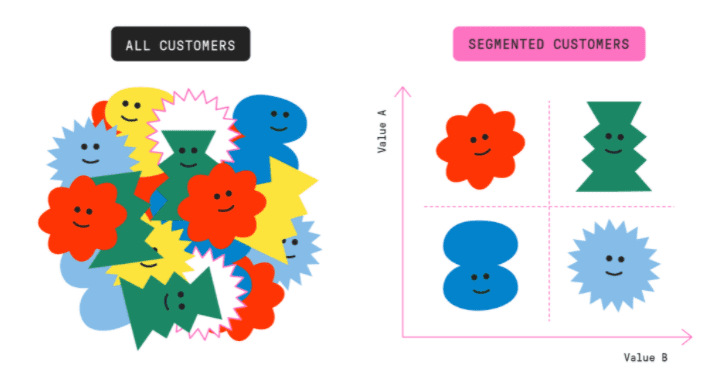
\includegraphics[width=0.75\textwidth]{images/gambar-6-2-2-customer-segmentation.png}}
\caption{Segmentasi pelanggan memakai unsupervised learning untuk mengenali kelompok karakteristik nasabah \cite{han2011}.}
\label{fig:customer-seg}
\end{figure}


\section{Konsep Dasar Klasterisasi}
Klasterisasi membagi sekumpulan objek observasi ke dalam sejumlah kelompok atau klaster. Analisis klaster berpegang pada dua kriteria geometris:
\begin{enumerate}
    \item \textbf{Intra-cluster similarity tinggi:} Titik data di dalam kelompok yang sama saling berdekatan dan memiliki karakteristik fitur yang serupa.
    \item \textbf{Inter-cluster dissimilarity tinggi:} Titik data yang berada pada kelompok berbeda terpisah jauh dengan perbedaan karakteristik yang tegas.
\end{enumerate}

Metode klasterisasi dapat dikelompokkan ke dalam tiga kategori utama:
\begin{itemize}
    \item \textbf{Partitional Clustering:} Membagi ruang data secara langsung ke dalam $K$ kelompok tanpa struktur bertingkat, contohnya K-Means dan K-Medoids.
    \item \textbf{Density-Based Clustering:} Membentuk kelompok berdasarkan daerah dengan kepadatan titik data tinggi yang dipisahkan oleh daerah renggang, contohnya DBSCAN.
    \item \textbf{Hierarchical Clustering:} Membangun struktur pohon klaster (dendrogram) secara aglomeratif (penggabungan dari bawah) atau divisif (pembagian dari atas).
\end{itemize}


\section{Algoritma K-Means}
Algoritma K-Means mempartisi $n$ data observasi ke dalam $K$ klaster berdasarkan jarak terdekat terhadap titik pusat massa rata-rata (centroid) \cite{macqueen1967}. Konsep partisi ruang fitur K-Means tampak pada Gambar~\ref{fig:kmeans-concept}.

\begin{figure}[H]
\centering
\fbox{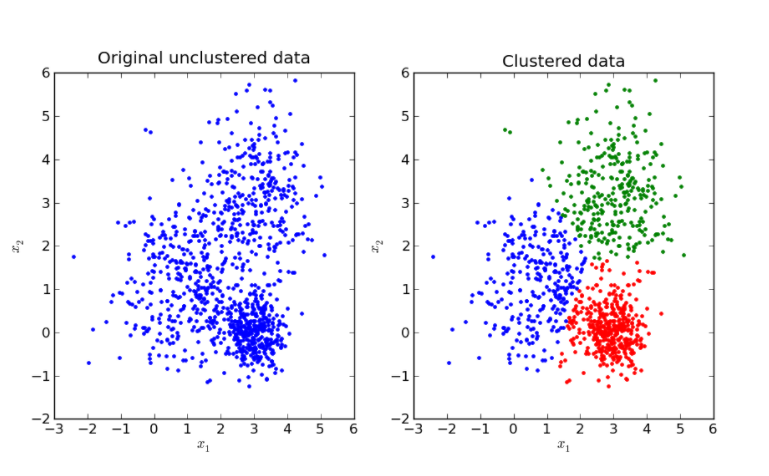
\includegraphics[width=0.7\textwidth]{images/gambar-6-2-3-k-means-concept.png}}
\caption{Konsep partisi ruang fitur pada algoritma K-Means \cite{bishop2006}.}
\label{fig:kmeans-concept}
\end{figure}

Tahapan algoritma K-Means berjalan secara berulang:
\begin{enumerate}
    \item \textbf{Inisialisasi Centroid:} Menentukan jumlah klaster $K$, kemudian memilih $K$ titik awal secara acak di dalam ruang data sebagai koordinat centroid $\mu_1, \mu_2, \dots, \mu_K$.
    \item \textbf{Penetapan Titik (Assignment Step):} Menghitung jarak Euclidean dari setiap titik $x_i$ ke masing-masing centroid $\mu_j$:
    \begin{equation}
    d(x_i, \mu_j) = \sqrt{\sum_{f=1}^{d} (x_{i,f} - \mu_{j,f})^2}
    \end{equation}
    Setiap titik dialokasikan ke klaster dengan centroid terdekat, seperti diilustrasikan pada Gambar~\ref{fig:kmeans-step1}.
    \item \textbf{Pembaruan Centroid (Update Step):} Menghitung ulang koordinat centroid $\mu_j$ sebagai rata-rata aritmetika (mean vector) dari seluruh titik anggota klaster $C_j$:
    \begin{equation}
    \mu_j = \frac{1}{|C_j|} \sum_{x \in C_j} x
    \end{equation}
    Proses pembaruan posisi centroid ini tampak pada Gambar~\ref{fig:kmeans-step2}.
    \item \textbf{Konvergensi:} Mengulang langkah kedua dan ketiga hingga posisi centroid tidak lagi berpindah secara signifikan, seperti terlihat pada Gambar~\ref{fig:kmeans-conv}.
\end{enumerate}

\begin{figure}[H]
\centering
\begin{minipage}[b]{0.48\textwidth}
    \centering
    \customfbox{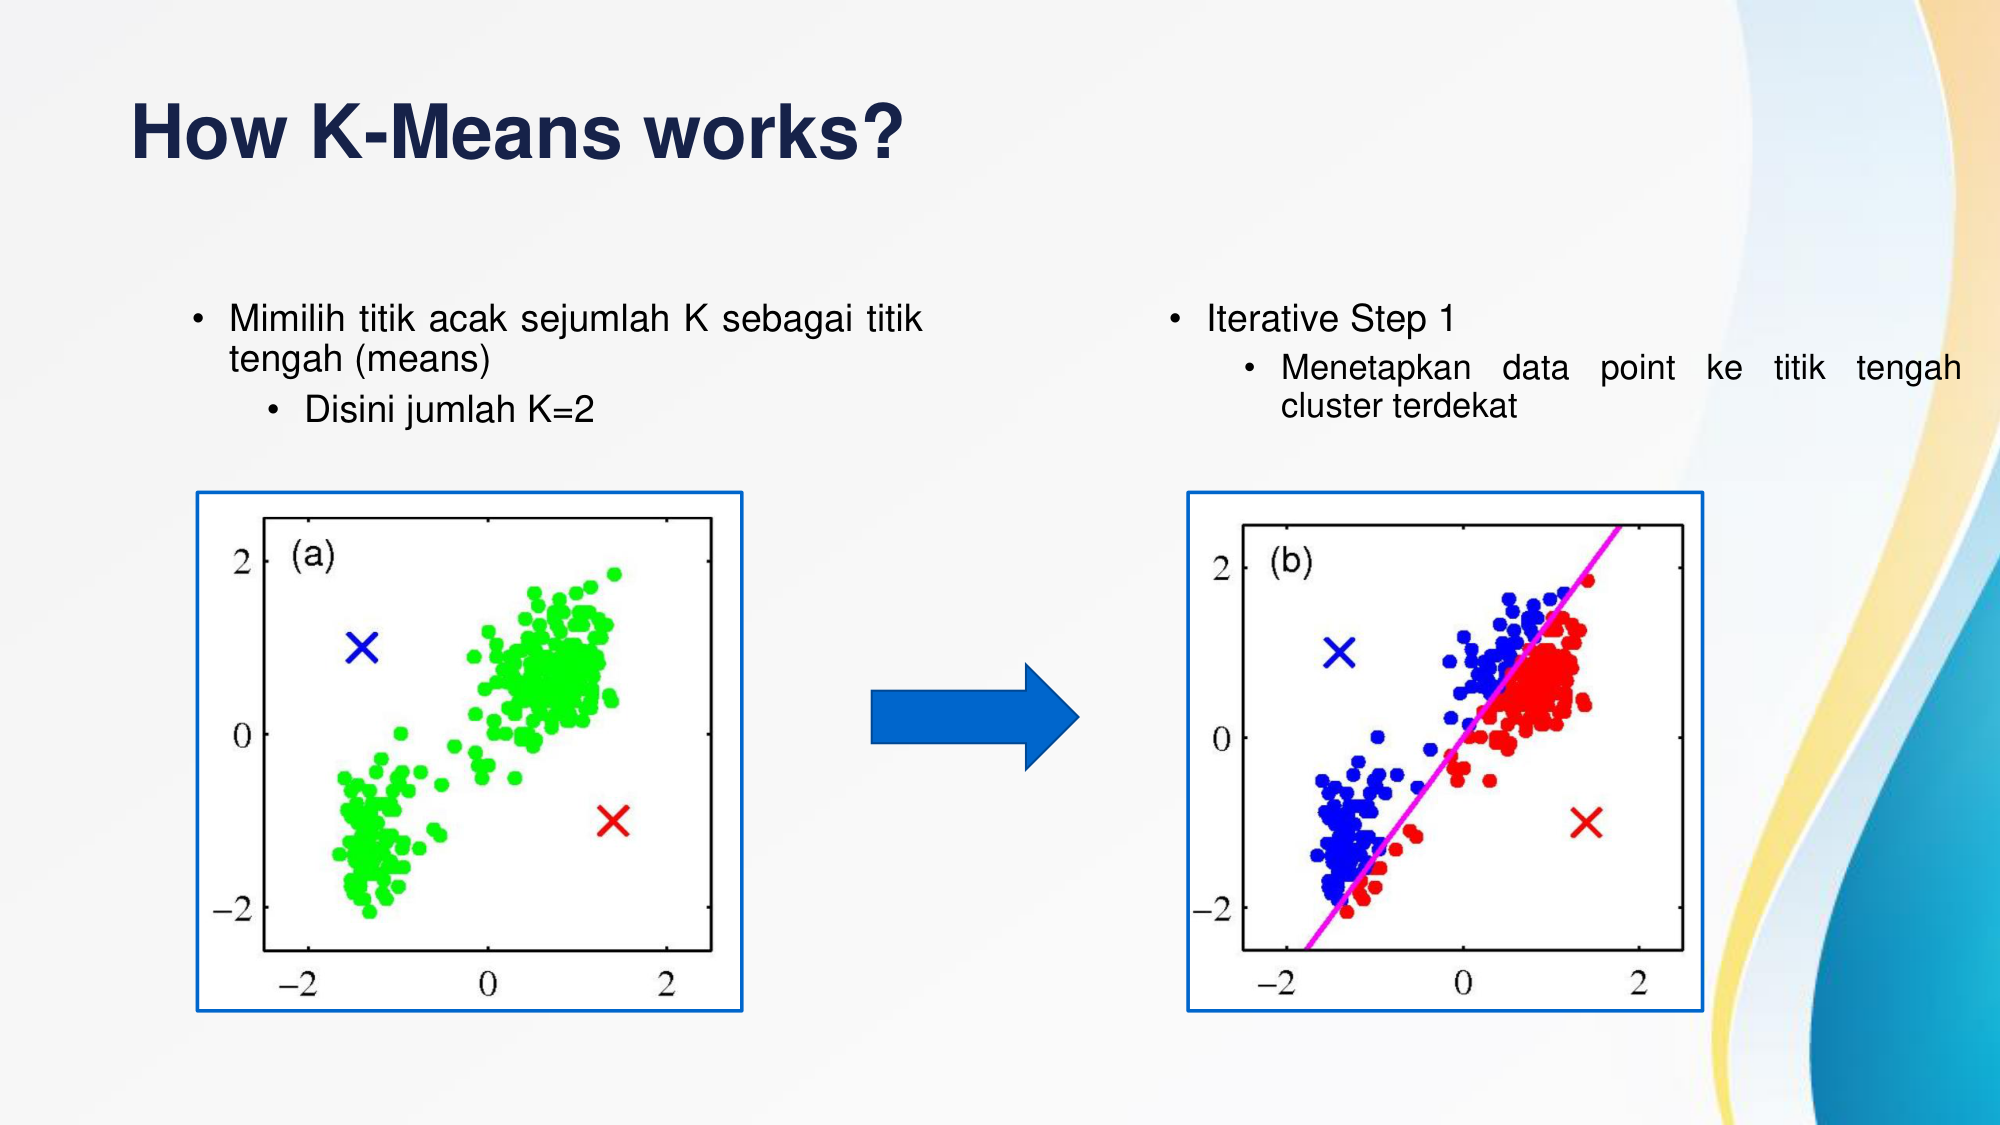
\includegraphics[width=\dimexpr\linewidth-1pt\relax]{images/gambar-6-2-4-k-means-step-1.png}}
    \caption{Penentuan centroid awal dan penetapan titik terdekat \cite{tan2019}.}
    \label{fig:kmeans-step1}
\end{minipage}
\hfill
\begin{minipage}[b]{0.48\textwidth}
    \centering
    \customfbox{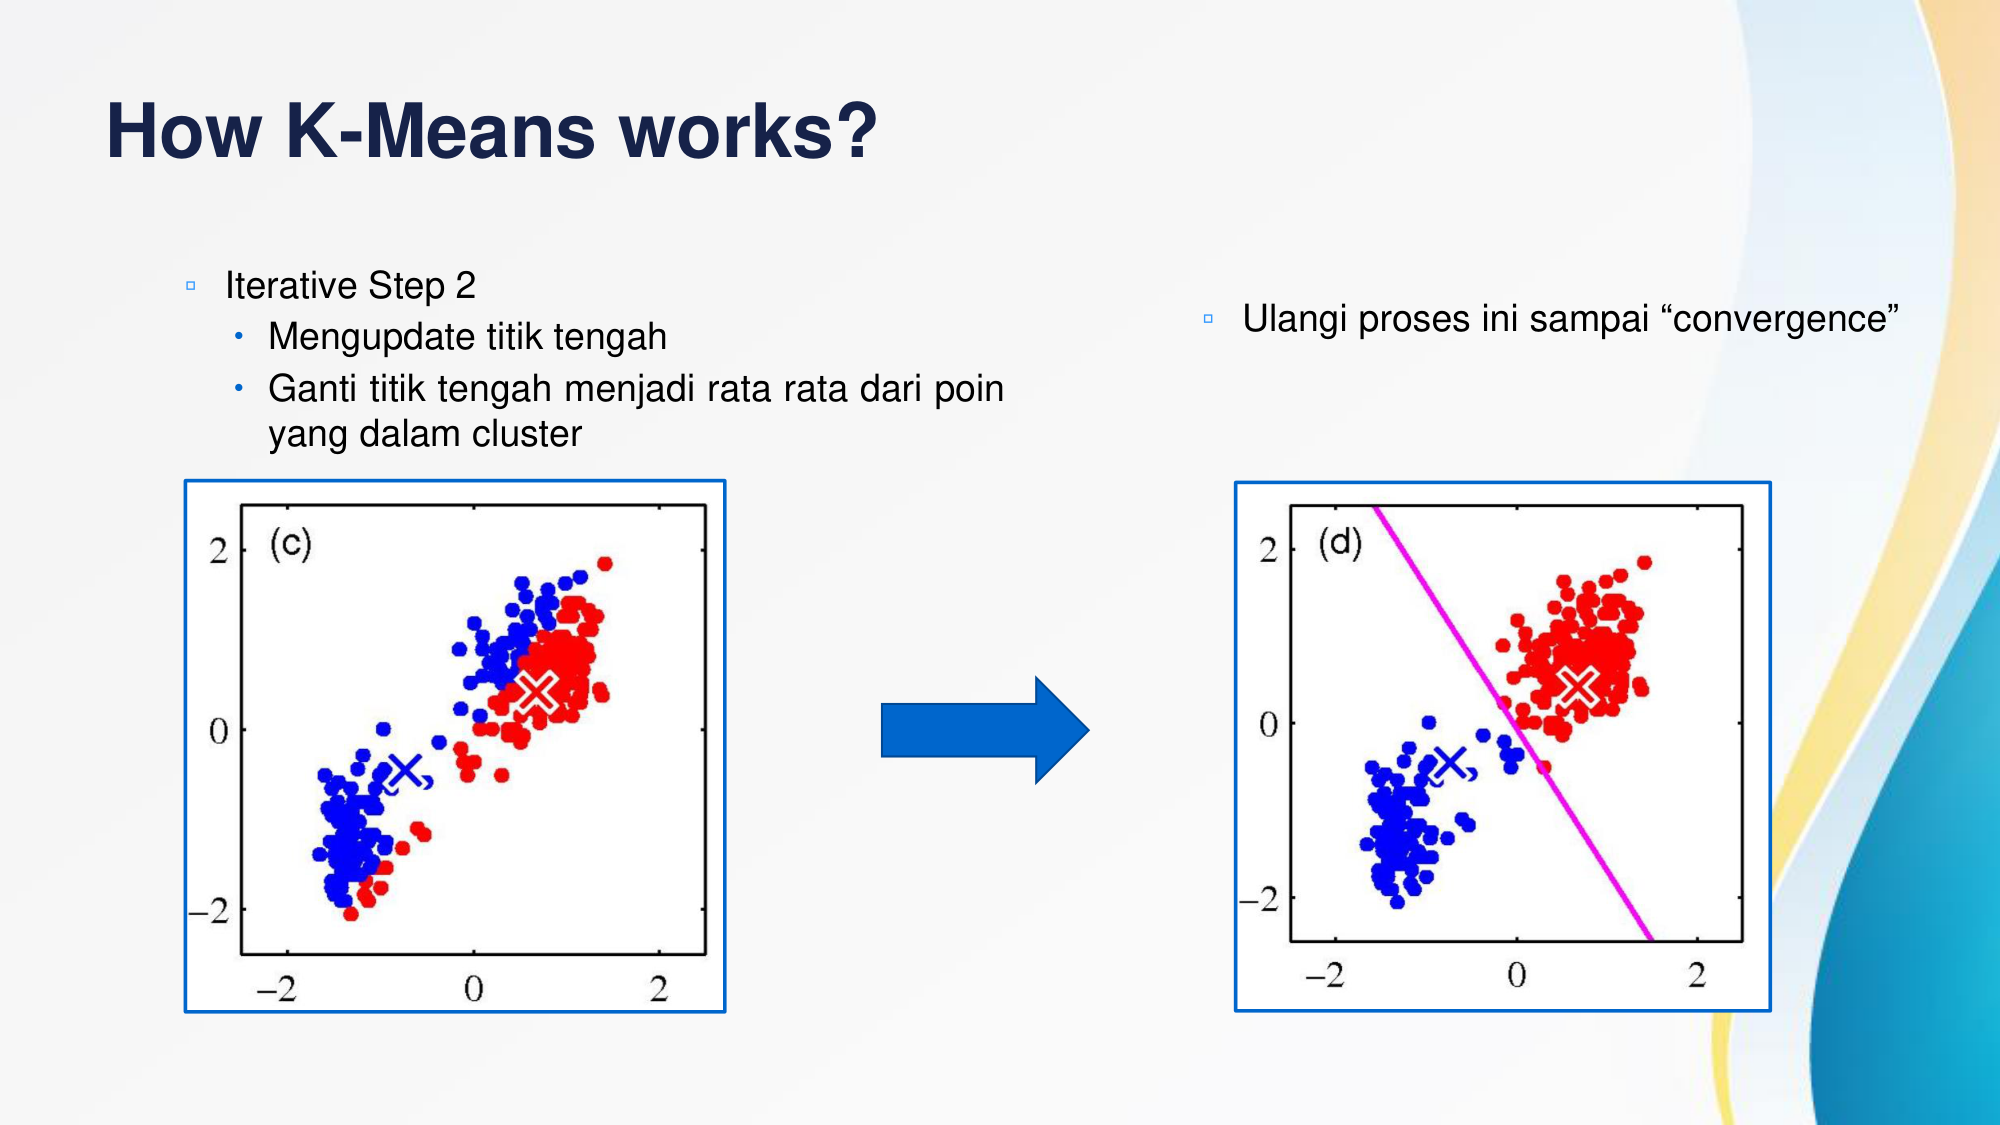
\includegraphics[width=\dimexpr\linewidth-1pt\relax]{images/gambar-6-2-5-k-means-step-2.png}}
    \caption{Pembaruan centroid berdasarkan rata-rata anggota klaster \cite{tan2019}.}
    \label{fig:kmeans-step2}
\end{minipage}
\end{figure}

\begin{figure}[H]
\centering
\fbox{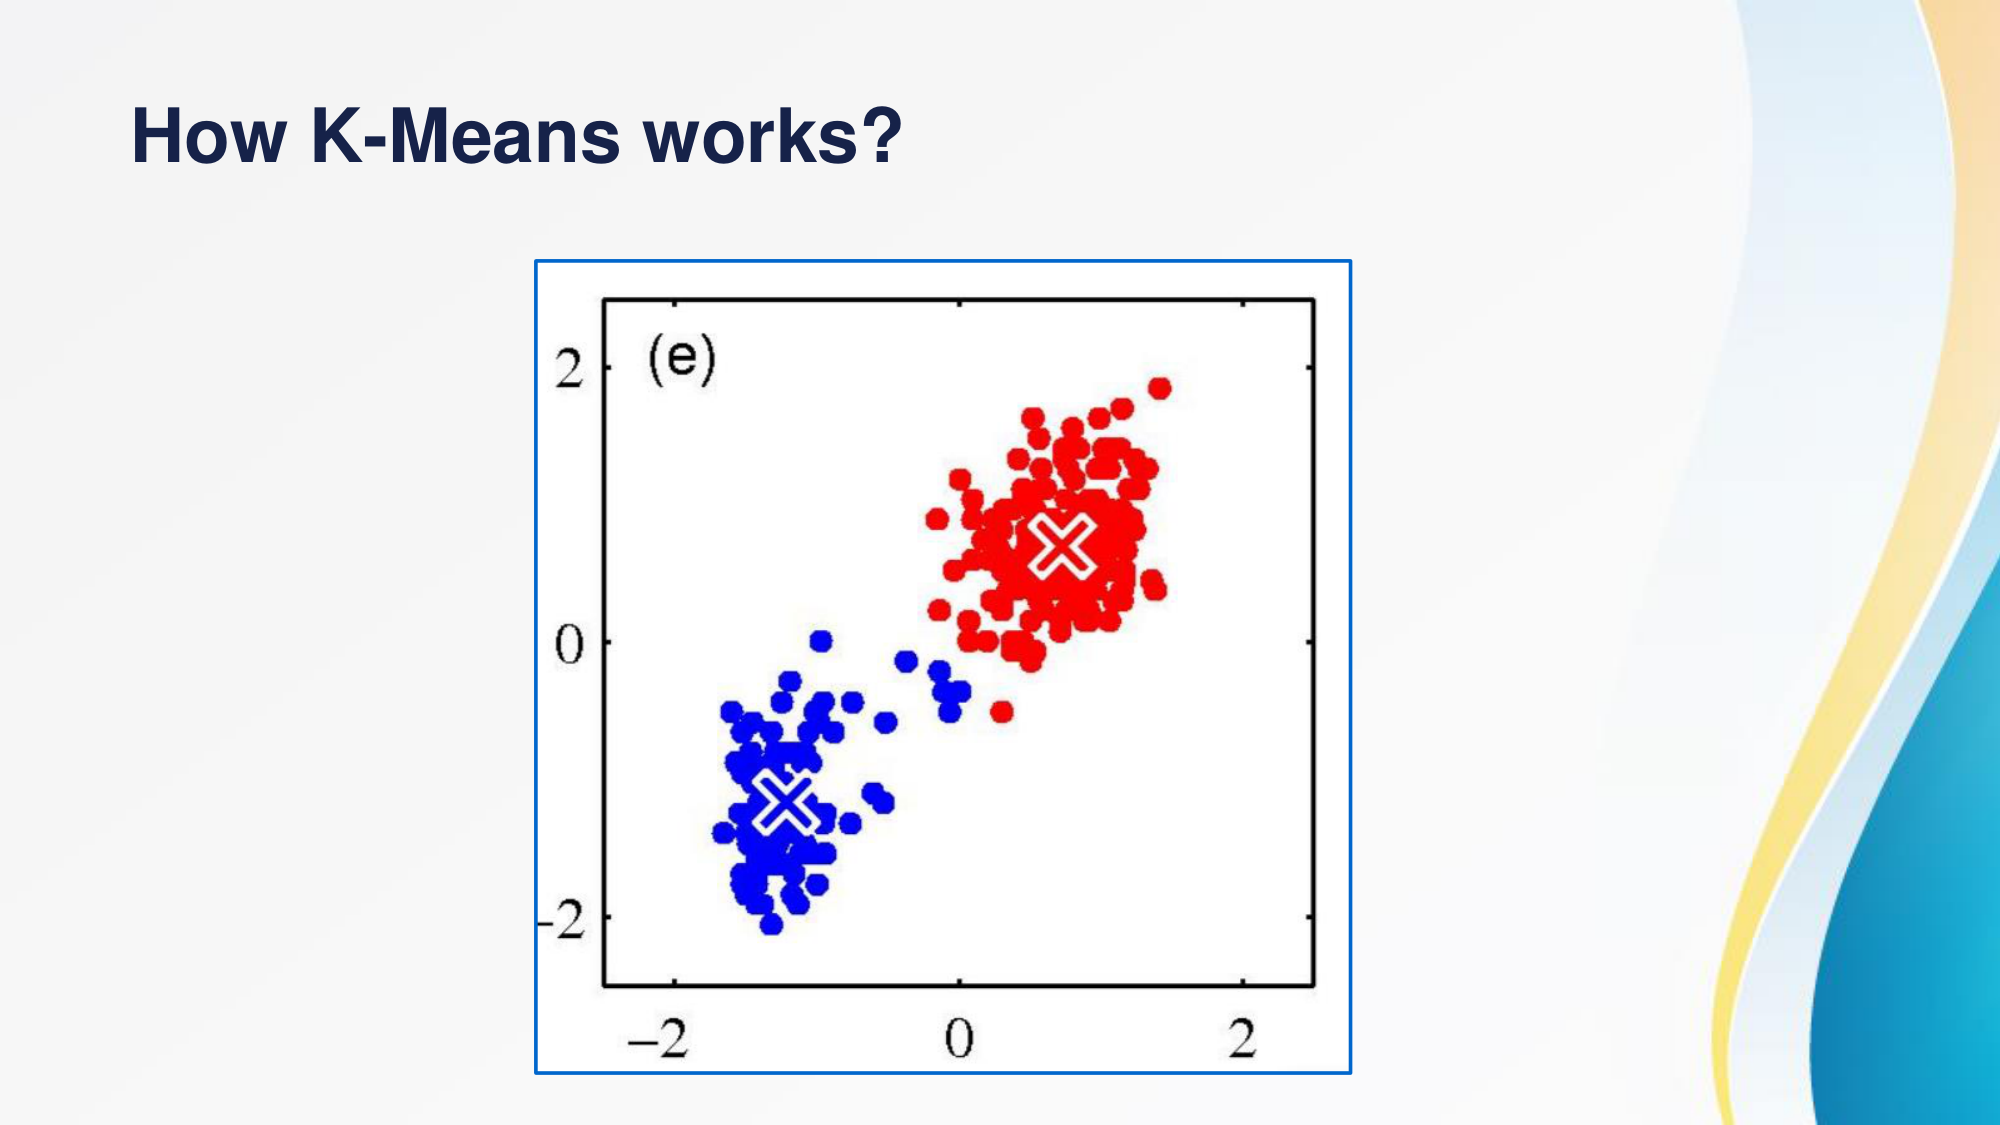
\includegraphics[width=0.62\textwidth]{images/gambar-6-2-6-k-means-convergence.png}}
\caption{Kondisi konvergensi K-Means saat posisi partisi klaster telah stabil \cite{tan2019}.}
\label{fig:kmeans-conv}
\end{figure}

K-Means memiliki waktu komputasi yang efisien berorde $O(t \cdot K \cdot n \cdot d)$, dengan $t$ jumlah iterasi, $K$ jumlah klaster, $n$ jumlah sampel, dan $d$ dimensi fitur \cite{han2011}. Namun K-Means memiliki kelemahan:
\begin{itemize}[noitemsep, topsep=2pt, parsep=1pt]
    \item Nilai $K$ harus ditentukan sebelum algoritma dijalankan.
    \item Hasil pengelompokan dapat terjebak pada optimum lokal karena sensitif terhadap pemilihan lokasi centroid awal.
    \item K-Means mengasumsikan klaster berbentuk bola cembung (spherical) dengan ukuran yang seimbang, sehingga gagal pada data dengan pola bergelombang atau cincin.
    \item K-Means sensitif terhadap nilai pencilan (outlier). Karena centroid dihitung memakai rata-rata aritmetika, satu nilai ekstrem dapat menarik posisi centroid menjauh dari kumpulan data utama, seperti tampak pada Gambar~\ref{fig:kmeans-outlier}.
\end{itemize}

\begin{figure}[H]
\centering
\fbox{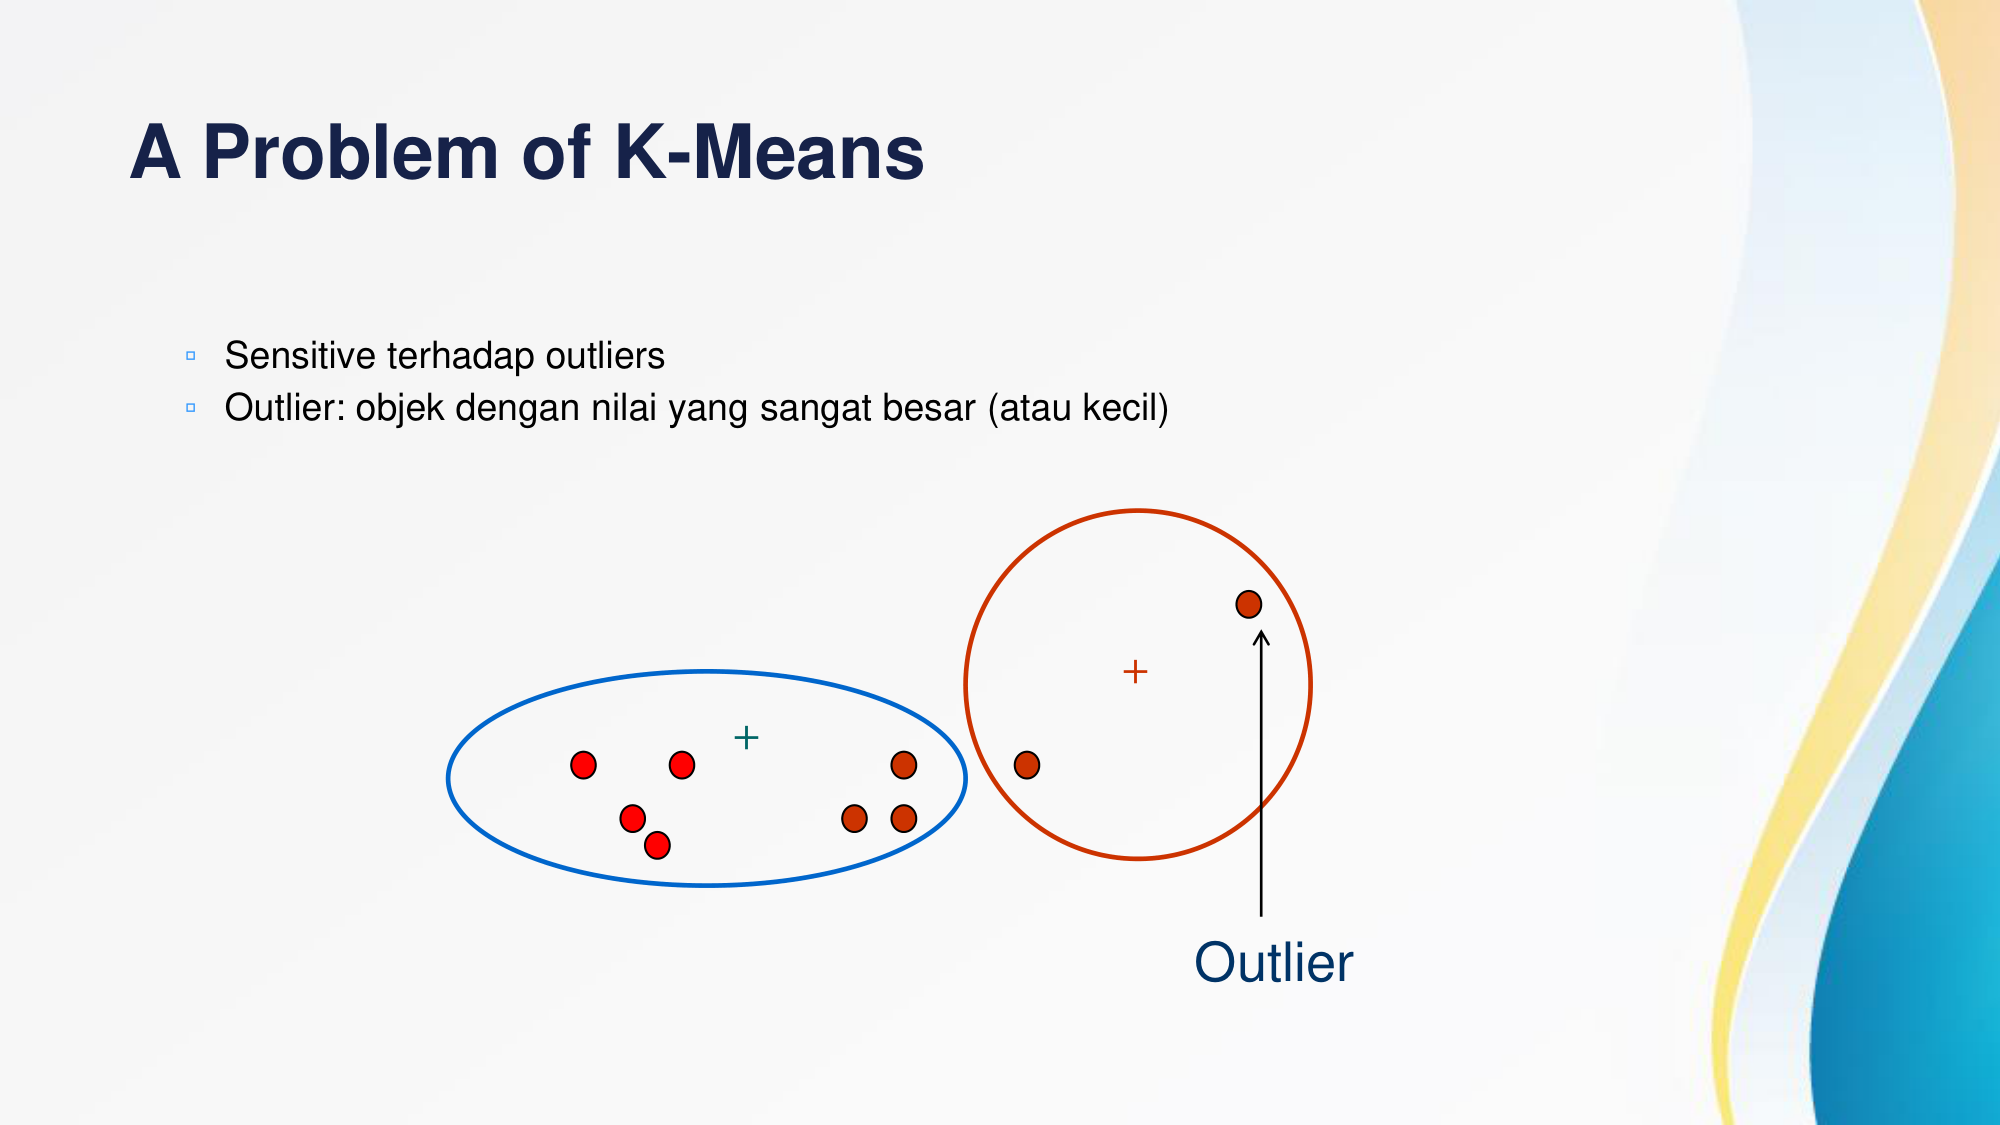
\includegraphics[width=0.65\textwidth]{images/gambar-6-2-7-k-means-outlier-problem.png}}
\caption{Pengaruh data pencilan yang menggeser posisi centroid pada K-Means \cite{tan2019}.}
\label{fig:kmeans-outlier}
\end{figure}

\section{Evaluasi Kualitas Klaster dan Penentuan Nilai K}
Evaluasi klaster pada data tanpa label dilakukan memakai kriteria evaluasi internal, yaitu Inertia dan Silhouette Score.

\subsection{Inertia (Within-Cluster Sum of Squares)}
Inertia mengukur tingkat kerapatan titik data di sekitar centroid klasternya. Nilai ini dihitung sebagai jumlah kuadrat jarak Euclidean antara setiap titik dengan centroid klaster terdekatnya:
\begin{equation}
\text{Inertia} = \sum_{j=1}^{K} \sum_{x_i \in C_j} ||x_i - \mu_j||^2
\end{equation}
Nilai inertia selalu menurun ketika nilai $K$ dinaikkan. Pada kondisi ekstrem saat $K = n$, inertia bernilai nol. Oleh karena itu, penurunan inertia dianalisis memakai grafik Elbow Method untuk mencari titik perubahan laju penurunan.

\subsection{Silhouette Score}
Silhouette Score mengukur tingkat pemisahan antar-klaster dibandingkan dengan kerapatan di dalam klaster sendiri \cite{rousseeuw1987}. Untuk sampel $i$, koefisien siluet dihitung melalui:
\begin{equation}
s(i) = \frac{b(i) - a(i)}{\max(a(i), b(i))}
\end{equation}
dengan $a(i)$ menyatakan rata-rata jarak titik $i$ ke semua titik lain di klaster yang sama, dan $b(i)$ menyatakan rata-rata jarak titik $i$ ke semua titik pada klaster tetangga terdekat.

Rentang nilai Silhouette Score berada pada interval $[-1, 1]$:
\begin{itemize}[noitemsep, topsep=2pt, parsep=1pt]
    \item Nilai mendekati 1 menunjukkan titik berada jauh dari klaster lain dan berdekatan dengan anggota kelompoknya.
    \item Nilai di sekitar 0 menandakan titik berada pada perbatasan antar-klaster.
    \item Nilai bernilai negatif menunjukkan titik kemungkinan dialokasikan pada klaster yang keliru karena jaraknya lebih dekat ke klaster lain.
\end{itemize}

\subsection{Penentuan Nilai K Optimal}
Dua metode utama dipakai untuk menentukan nilai $K$ optimal:
\begin{enumerate}[noitemsep, topsep=2pt, parsep=1pt]
    \item \textbf{Elbow Method:} Membuat plot grafik inertia terhadap variasi nilai $K$. Titik siku (elbow point) dipilih pada posisi di mana penurunan inertia mulai melambat secara nyata, seperti diilustrasikan pada Gambar~\ref{fig:elbow-silhouette}.
    \item \textbf{Deteksi Siku Otomatis (KneeLocator):} Algoritma `kneed` menghitung kelengkungan maksimum kurva secara matematis untuk menemukan titik siku tanpa bias penglihatan manusia \cite{satopaa2011}.
    \item \textbf{Silhouette Analysis:} Memilih nilai $K$ yang menghasilkan rata-rata skor siluet tertinggi di antara rentang uji.
\end{enumerate}

\begin{figure}[H]
\centering
\fbox{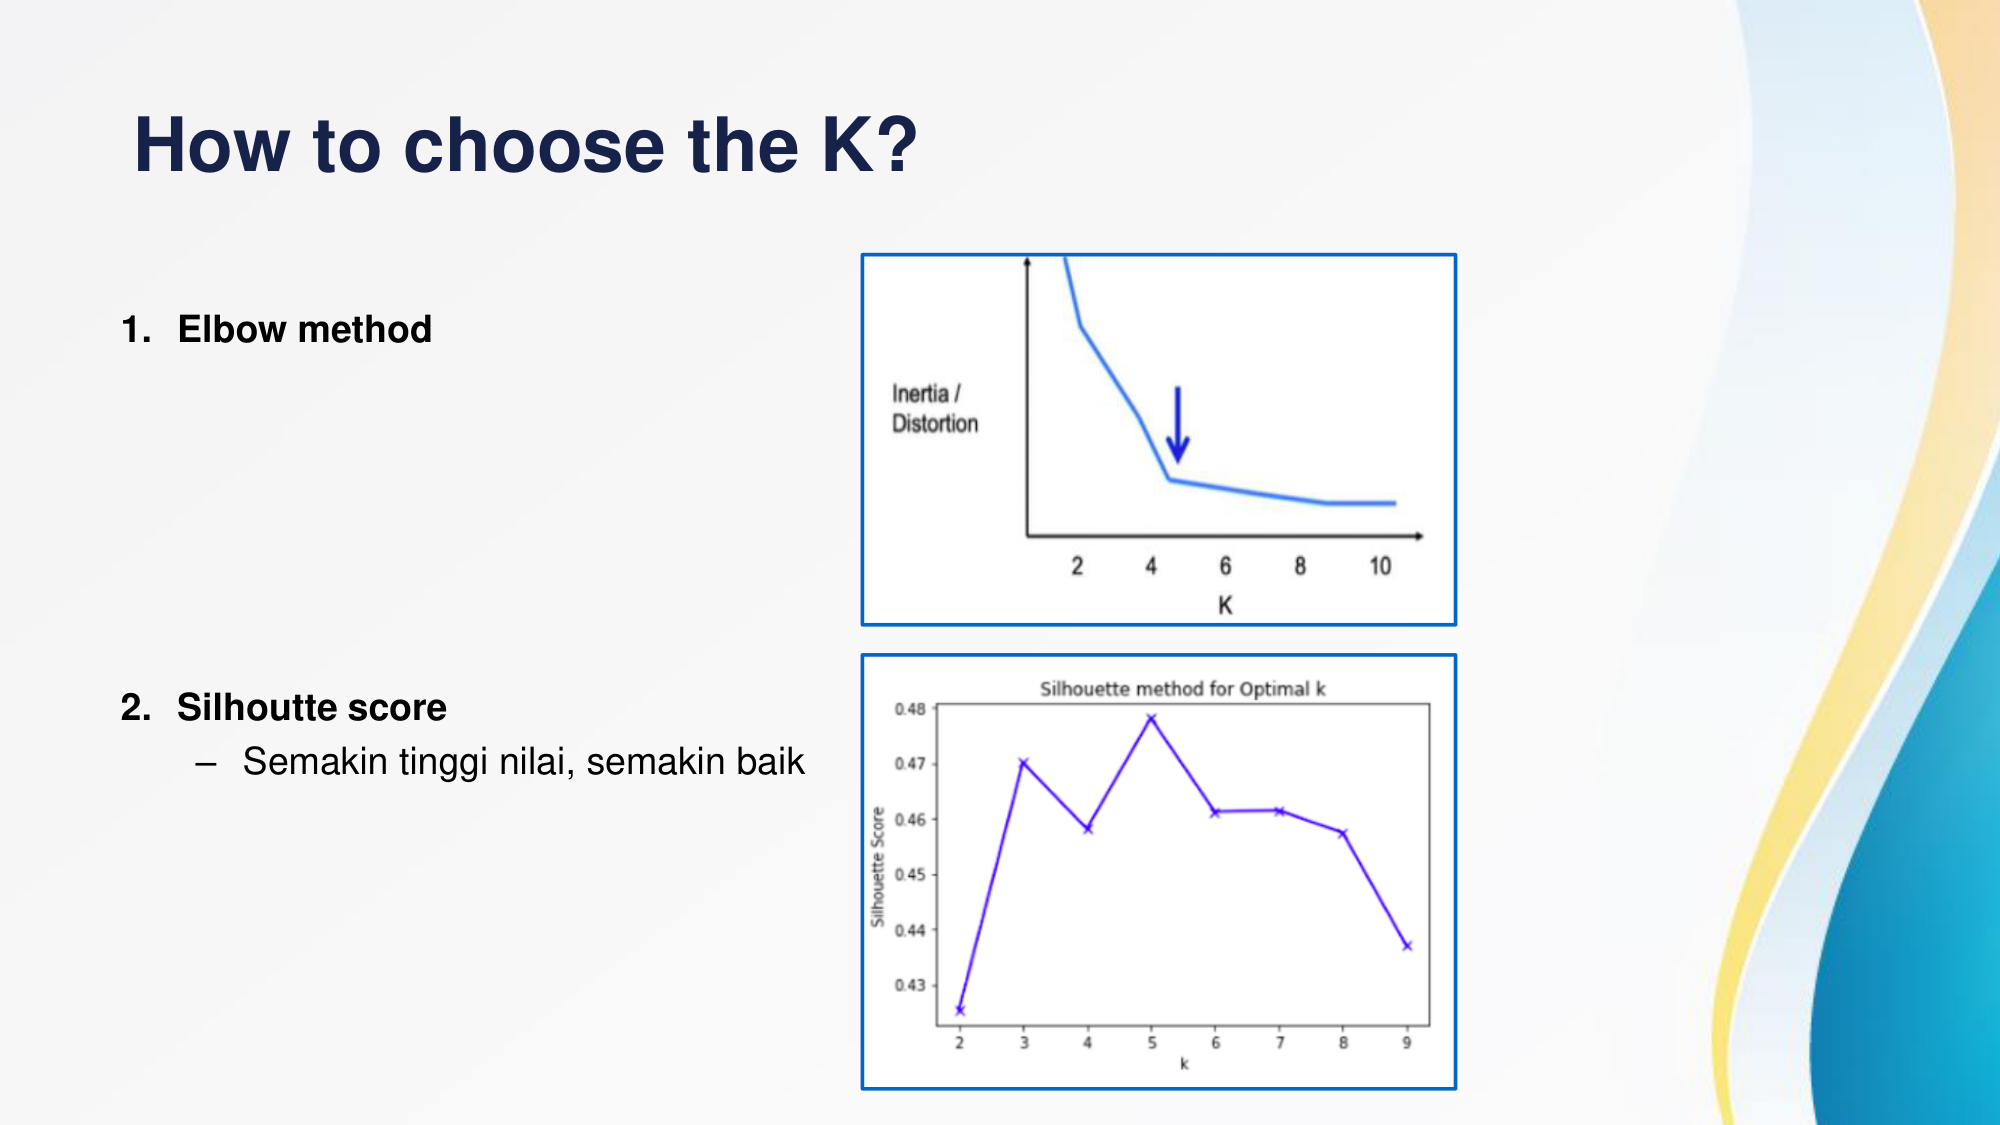
\includegraphics[width=0.68\textwidth]{images/gambar-6-2-7b-menentukan-k-elbow-silhouette.png}}
\caption{Penentuan jumlah klaster optimal memakai kurva Elbow dan Silhouette Score \cite{han2011}.}
\label{fig:elbow-silhouette}
\end{figure}

\section{Algoritma K-Medoids (Partitioning Around Medoids)}
Algoritma K-Medoids atau PAM dikembangkan oleh Leonard Kaufman dan Peter J. Rousseeuw pada tahun 1990 untuk mengatasi kelemahan K-Means terhadap pencilan \cite{kaufman1990}. K-Medoids memakai titik data riil dari dataset sebagai representasi pusat klaster (medoid), bukan rata-rata imajiner seperti pada K-Means. Perbedaan kedua titik pusat ini tampak pada Gambar~\ref{fig:kmed-vs-kmeans}.

\begin{figure}[H]
\centering
\fbox{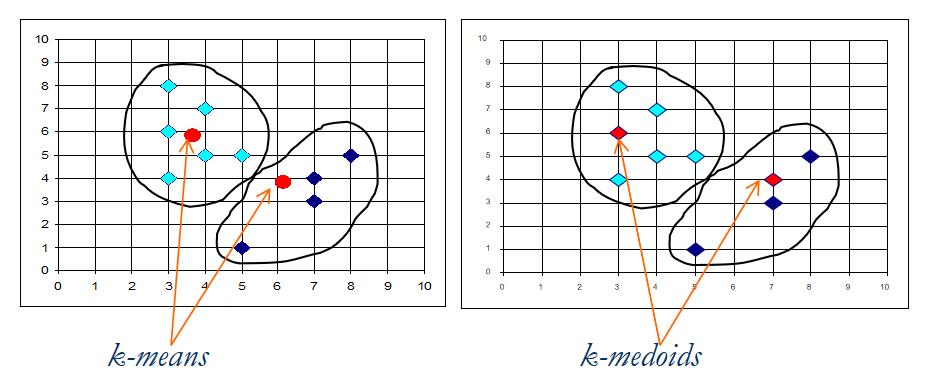
\includegraphics[width=0.68\textwidth]{images/gambar-6-2-8-k-medoids-vs-k-means.png}}
\caption{Perbedaan titik pusat: K-Means memakai rata-rata imajiner, sedangkan K-Medoids memakai data riil medoid \cite{kaufman1990}.}
\label{fig:kmed-vs-kmeans}
\end{figure}

Tabel~\ref{tab:kmeans-vs-kmedoids} merangkum perbandingan teknis antara K-Means dan K-Medoids.

\begin{table}[H]
\centering
\small
\begin{tabularx}{\textwidth}{>{\raggedright\arraybackslash}p{3cm} >{\raggedright\arraybackslash}X >{\raggedright\arraybackslash}X}
\toprule
\textbf{Karakteristik} & \textbf{K-Means} & \textbf{K-Medoids (PAM)} \\
\midrule
Pusat Klaster & Vektor rata-rata (mean imajiner) & Objek data aktual di dalam dataset (medoid) \\
Fungsi Objektif & Meminimalkan jumlah kuadrat galat (Euclidean) & Meminimalkan jumlah dissimilaritas absolut \\
Ketahanan Pencilan & Peka terhadap pencilan \cite{tan2019} & Tahan terhadap pencilan dan derau \cite{herviany2021} \\
Kompleksitas & Cepat, linier $O(t \cdot K \cdot n \cdot d)$ \cite{sulistiyawati2021} & Lebih berat, kuadratik $O(t \cdot K \cdot (n-K)^2)$ \\
\bottomrule
\end{tabularx}
\caption{Perbandingan karakteristik algoritma K-Means dan K-Medoids.}
\label{tab:kmeans-vs-kmedoids}
\end{table}

Prinsip kerja PAM meliputi:
\begin{enumerate}
    \item Memilih secara acak $K$ objek data riil sebagai medoid awal $M = \{m_1, \dots, m_K\}$.
    \item Menetapkan setiap objek non-medoid ke medoid terdekatnya.
    \item Mengevaluasi pertukaran medoid (swapping): untuk setiap medoid $m_i$ dan kandidat non-medoid $o_h$, posisi ditukar untuk sementara dan kriteria galat absolut total dihitung:
    \begin{equation}
    E = \sum_{i=1}^{K} \sum_{p \in C_i} |p - m_i|
    \end{equation}
    \item Menghitung perubahan biaya pertukaran $S = E_{\text{baru}} - E_{\text{lama}}$. Jika $S < 0$, pertukaran menurunkan total galat sehingga posisi medoid diperbarui secara permanen. Jika $S \ge 0$, pertukaran ditolak.
    \item Mengulang evaluasi hingga tidak ada lagi pertukaran yang menurunkan galat.
\end{enumerate}

Sebagai simulasi numerik pada sepuluh titik data dua dimensi: $O_1(2,6)$, $O_2(3,4)$, $O_3(3,8)$, $O_4(4,7)$, $O_5(6,2)$, $O_6(6,4)$, $O_7(7,3)$, $O_8(7,4)$, $O_9(8,5)$, dan $O_{10}(7,6)$. Untuk $K = 2$ dengan medoid awal $(O_2, O_8)$, total jarak pada klaster 1 bernilai 11 dan klaster 2 bernilai 9, sehingga $E_{\text{lama}} = 20$. Ketika medoid $O_8$ dicoba ditukar dengan $O_7(7,3)$, total jarak klaster 1 tetap 11 dan klaster 2 menjadi 11, sehingga $E_{\text{baru}} = 22$. Nilai biaya swapping menjadi:
\begin{equation}
S = E_{\text{baru}} - E_{\text{lama}} = 22 - 20 = +2
\end{equation}
Karena $S > 0$, pertukaran tersebut ditolak dan $O_8$ tetap dipertahankan sebagai medoid. Proses evaluasi ini diilustrasikan pada Gambar~\ref{fig:kmed-error} dan Gambar~\ref{fig:kmed-cost}.

\begin{figure}[H]
\centering
\begin{minipage}[b]{0.48\textwidth}
    \centering
    \customfbox{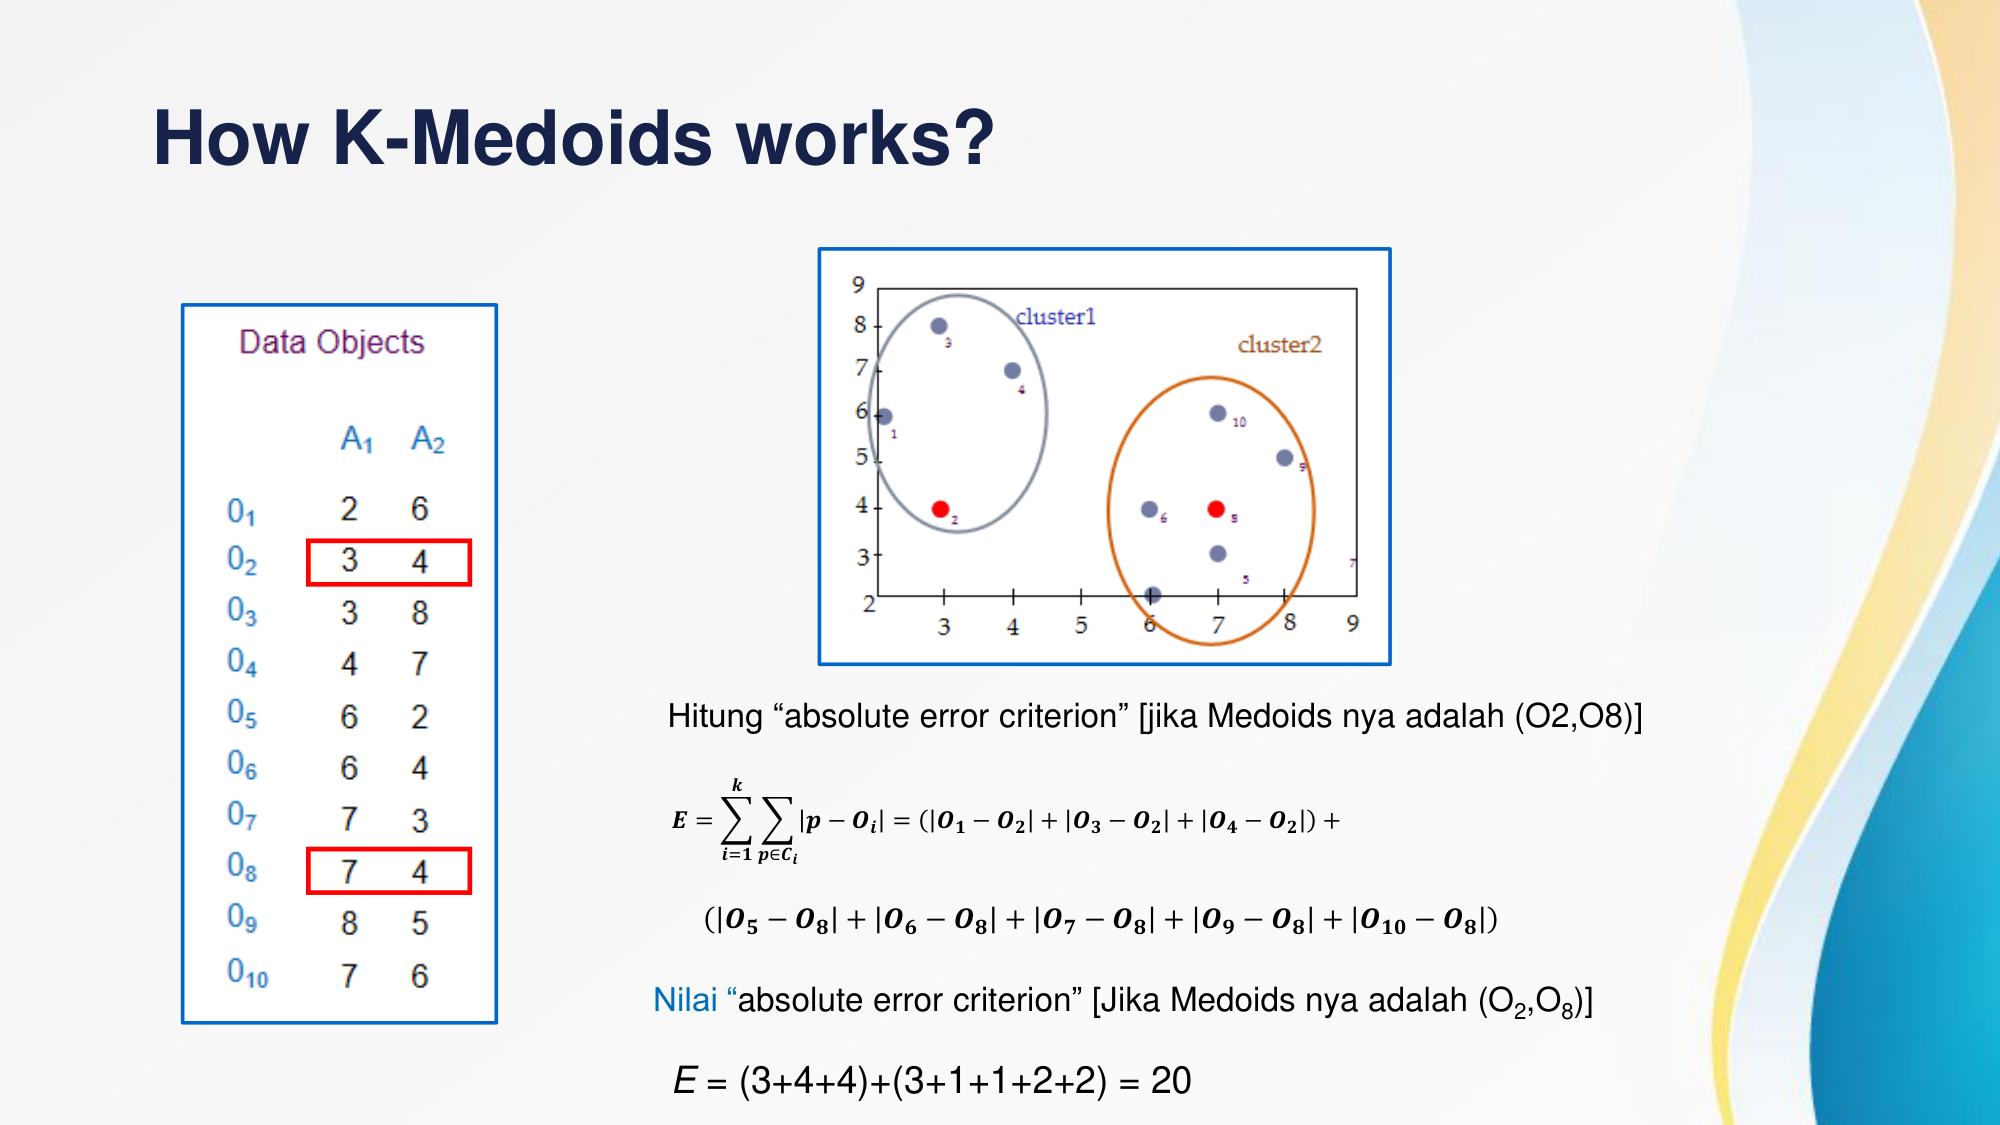
\includegraphics[width=\dimexpr\linewidth-1pt\relax]{images/gambar-6-2-10-k-medoids-pam-error-criterion.png}}
    \caption{Perhitungan galat absolut $E$ pada $(O_2, O_8)$ \cite{kaufman1990}.}
    \label{fig:kmed-error}
\end{minipage}
\hfill
\begin{minipage}[b]{0.48\textwidth}
    \centering
    \customfbox{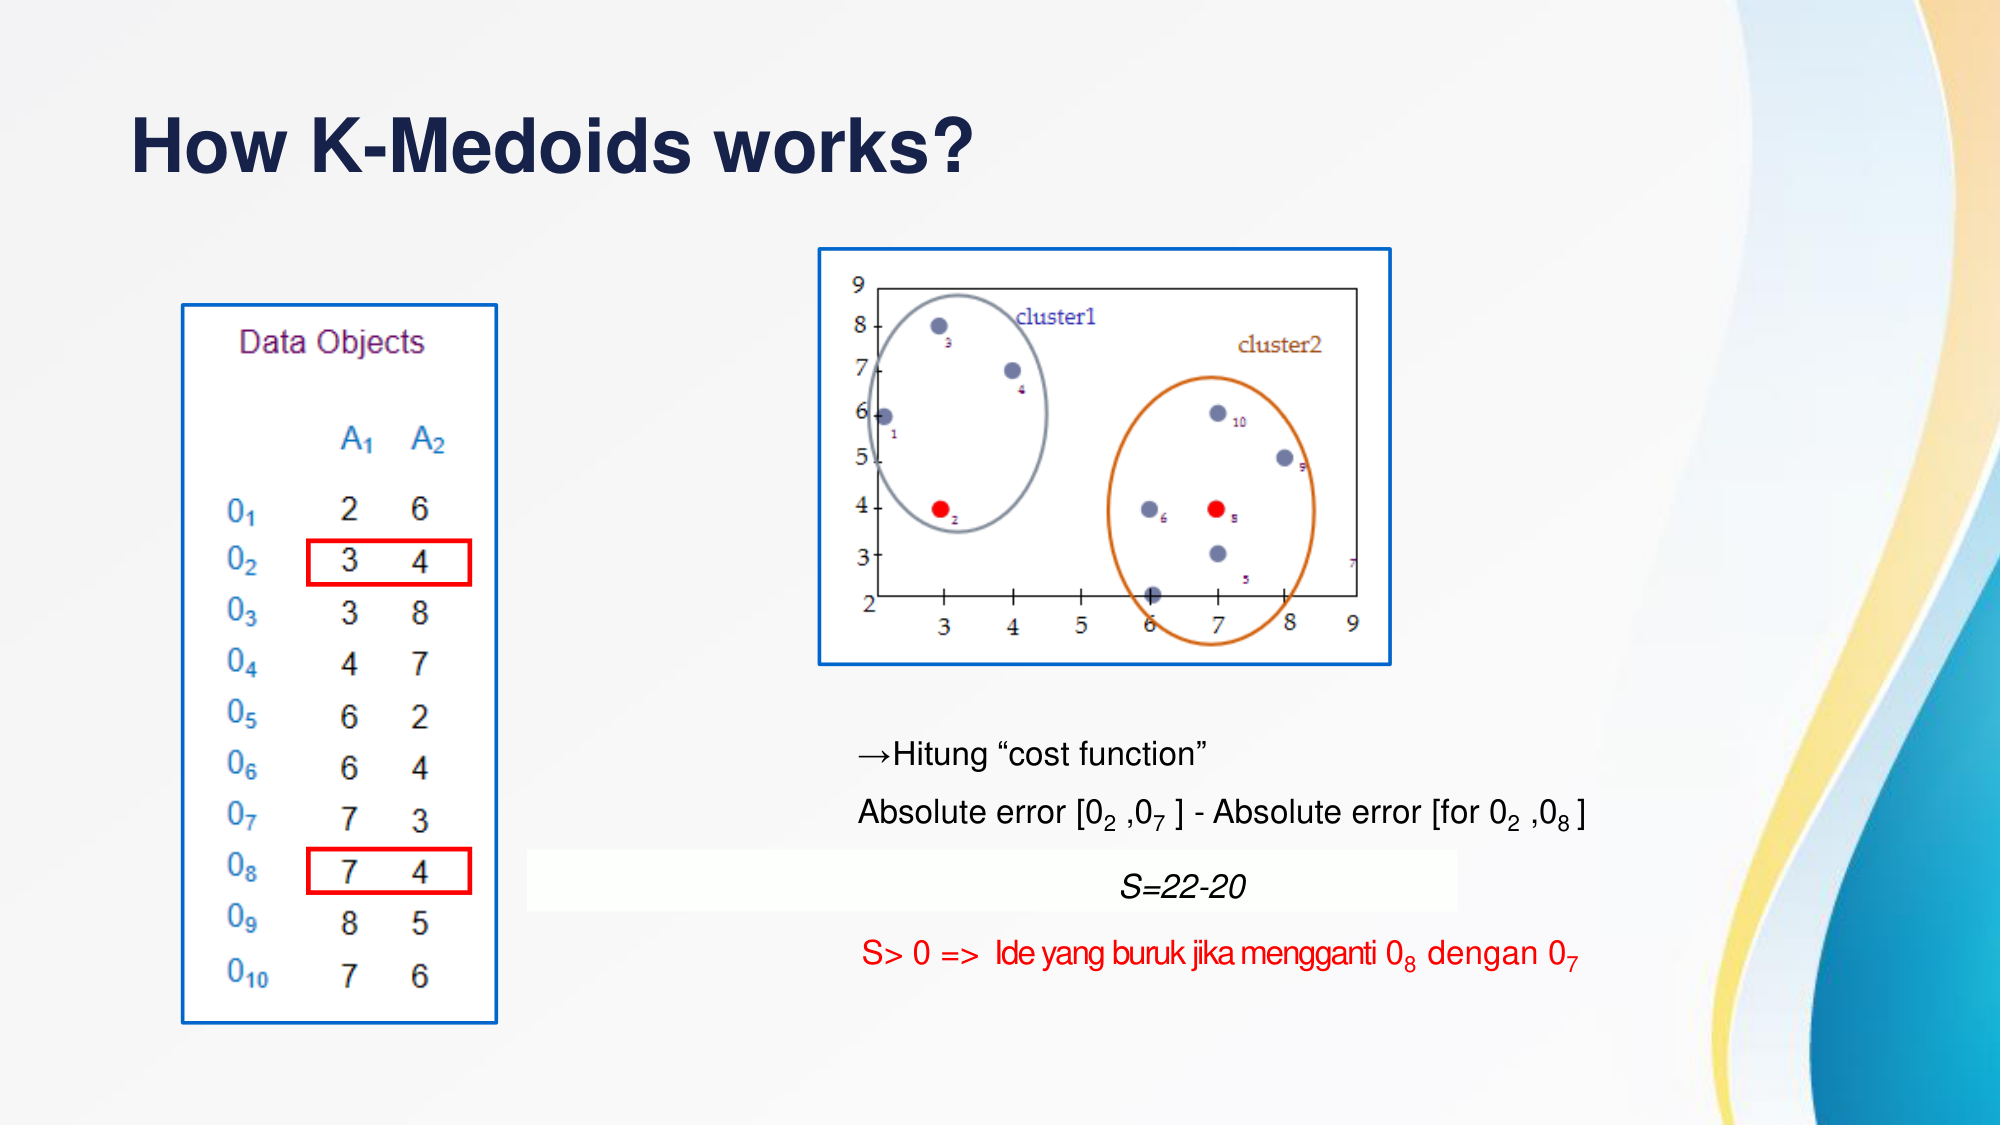
\includegraphics[width=\dimexpr\linewidth-1pt\relax]{images/gambar-6-2-11-k-medoids-pam-cost-function.png}}
    \caption{Evaluasi fungsi biaya pertukaran $S > 0$ \cite{kaufman1990}.}
    \label{fig:kmed-cost}
\end{minipage}
\end{figure}

\section{Algoritma DBSCAN}
Algoritma DBSCAN diusulkan oleh Martin Ester, Hans-Peter Kriegel, Jörg Sander, dan Xiaowei Xu pada tahun 1996 \cite{ester1996}. Algoritma ini dirancang untuk mendeteksi klaster dengan bentuk arbitrer dan memisahkan data pencilan secara otomatis. Ilustrasi konsep klasterisasi berbasis kerapatan tampak pada Gambar~\ref{fig:dbscan-concept}.

\begin{figure}[H]
\centering
\fbox{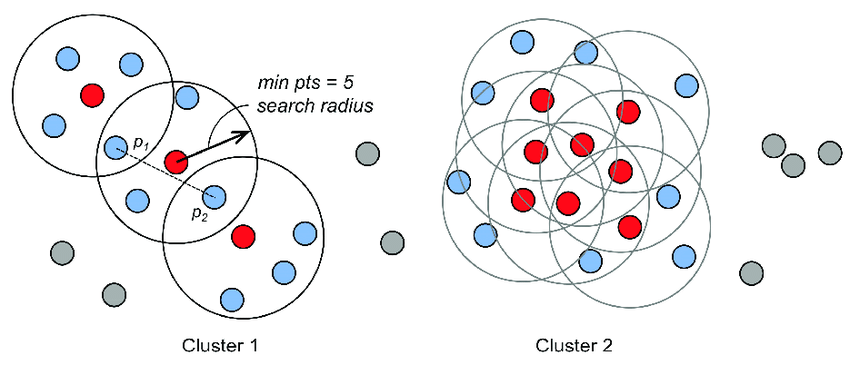
\includegraphics[width=0.68\textwidth]{images/gambar-6-2-12-dbscan-density-clusters.png}}
\caption{Konsep klasterisasi berbasis kepadatan spasial pada DBSCAN \cite{ester1996}.}
\label{fig:dbscan-concept}
\end{figure}

K-Means membagi data menjadi partisi sferis. Saat berhadapan dengan data yang membentuk cincin konsentris atau struktur bulan sabit, K-Means memotong kelompok menjadi irisan baji yang keliru. DBSCAN mengikuti rantai kerapatan titik, sehingga dapat membedakan cincin dalam dan cincin luar dengan benar serta mengisolasi pencilan sebagai noise, seperti tampak pada Gambar~\ref{fig:dbscan-why}.

\begin{figure}[H]
\centering
\fbox{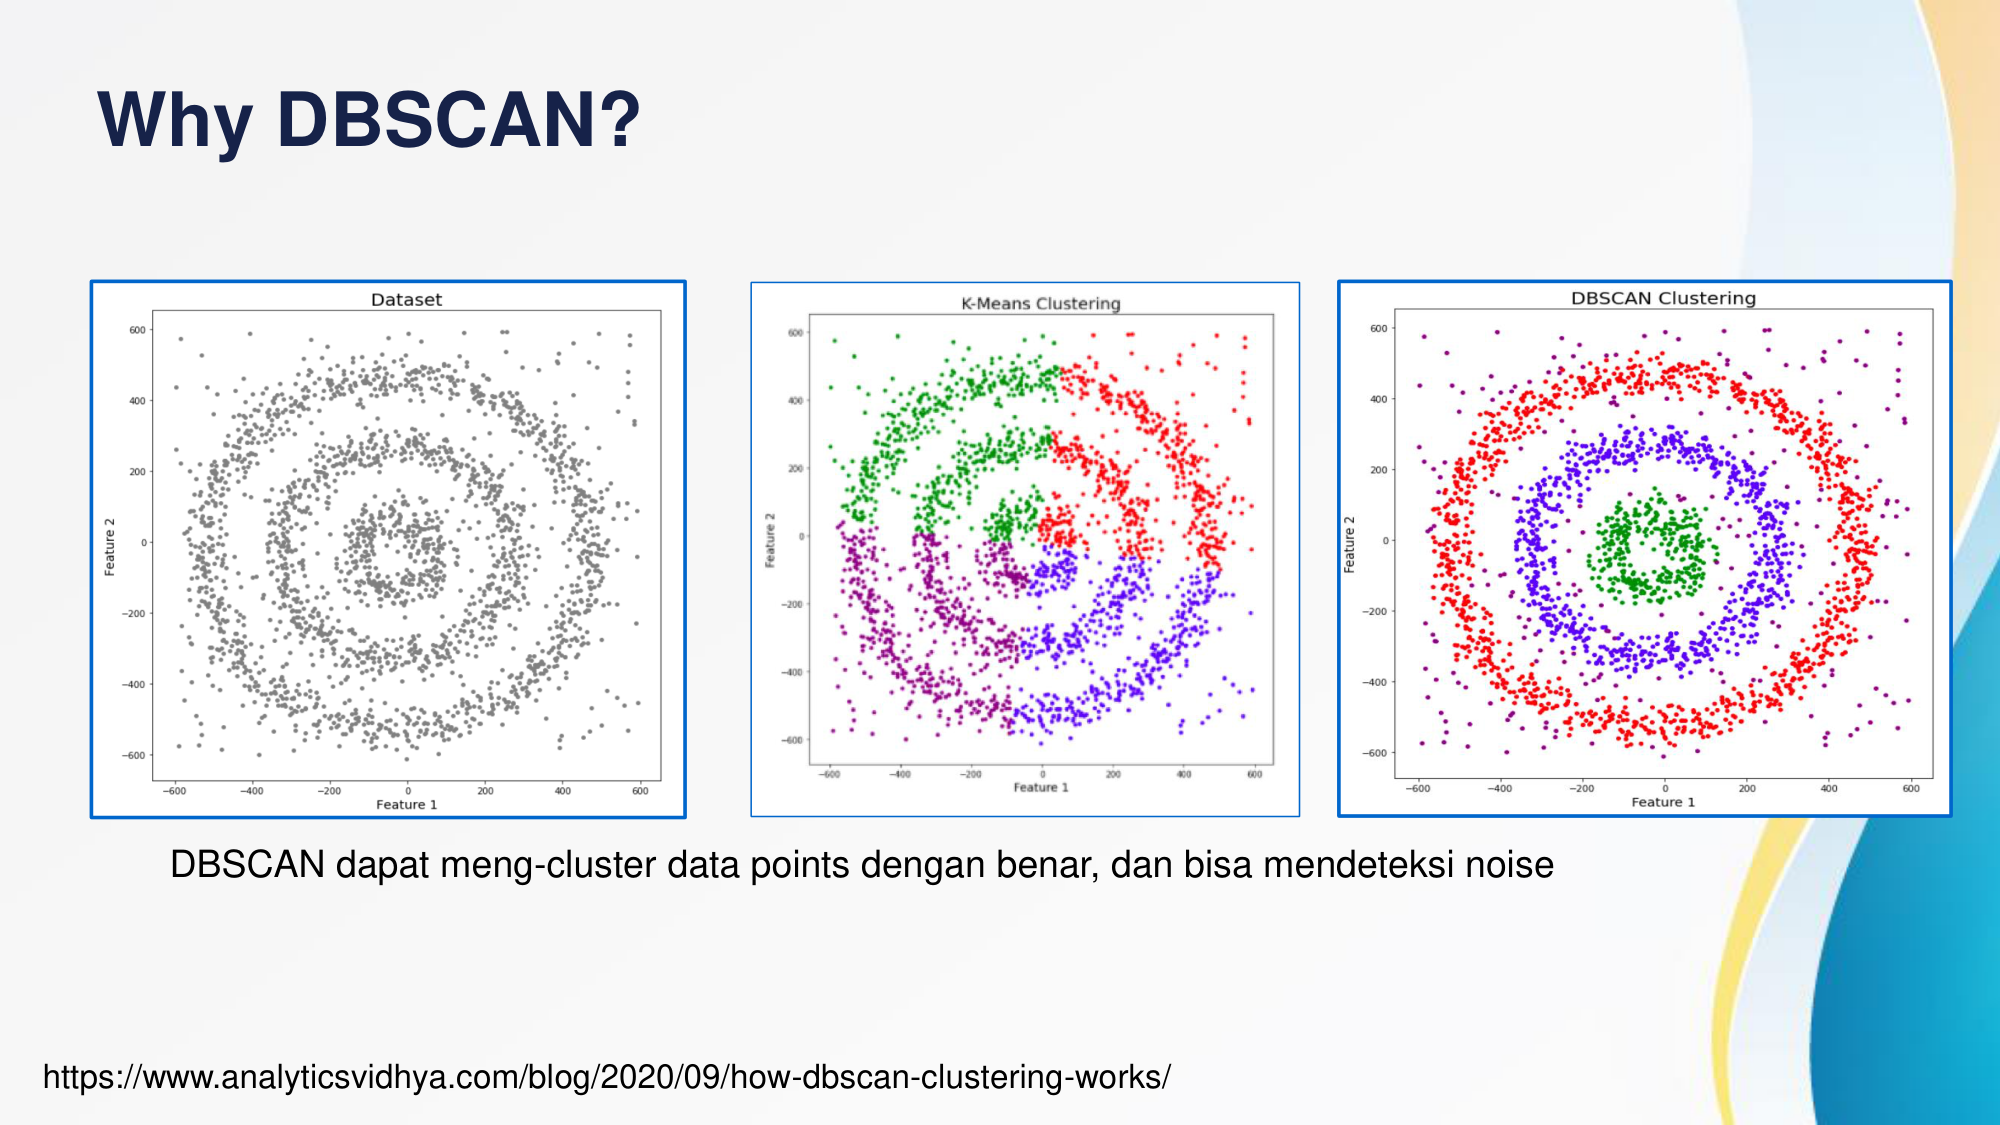
\includegraphics[width=0.65\textwidth]{images/gambar-6-2-13-why-dbscan-comparison.png}}
\caption{Perbandingan K-Means dan DBSCAN pada struktur data cincin konsentris \cite{ester1996}.}
\label{fig:dbscan-why}
\end{figure}

DBSCAN memakai dua parameter utama:
\begin{itemize}[noitemsep, topsep=2pt, parsep=1pt]
    \item $\epsilon$ (Epsilon): Radius jarak maksimum di sekitar suatu titik yang menjadi batas tetangga (neighborhood).
    \item $MinPts$ (Minimum Points): Jumlah minimum titik tetangga di dalam radius $\epsilon$ agar sebuah titik memenuhi kualifikasi sebagai titik inti (core point).
\end{itemize}

Definisi lingkungan dan titik inti:
\begin{itemize}[noitemsep, topsep=2pt, parsep=1pt]
    \item $\epsilon$-Neighborhood: $N_\epsilon(p) = \{q \in D \mid \text{dist}(p, q) \le \epsilon\}$.
    \item Titik Inti (Core Point): Titik $p$ yang memiliki setidaknya $MinPts$ tetangga, yaitu $|N_\epsilon(p)| \ge MinPts$.
    \item Directly Density-Reachable: Titik $p$ terjangkau langsung dari $q$ jika $q$ adalah core point dan $p \in N_\epsilon(q)$.
    \item Density-Reachable: Titik $p$ terjangkau melalui rantai titik perantara yang saling directly density-reachable dari $q$.
    \item Density-Connected: Titik $p$ dan $q$ sama-sama density-reachable dari satu titik inti $o$.
\end{itemize}

Berdasarkan definisi tersebut, titik pada DBSCAN dikelompokkan ke dalam tiga kategori:
\begin{enumerate}[noitemsep, topsep=2pt, parsep=1pt]
    \item \textbf{Core Point:} Memiliki minimal $MinPts$ tetangga di dalam radius $\epsilon$.
    \item \textbf{Border Point:} Berada di dalam radius $\epsilon$ dari titik inti, tetapi jumlah tetangganya kurang dari $MinPts$.
    \item \textbf{Noise Point:} Bukan titik inti dan tidak terjangkau oleh titik inti mana pun.
\end{enumerate}

\begin{figure}[H]
\centering
\begin{minipage}[b]{0.48\textwidth}
    \centering
    \customfbox{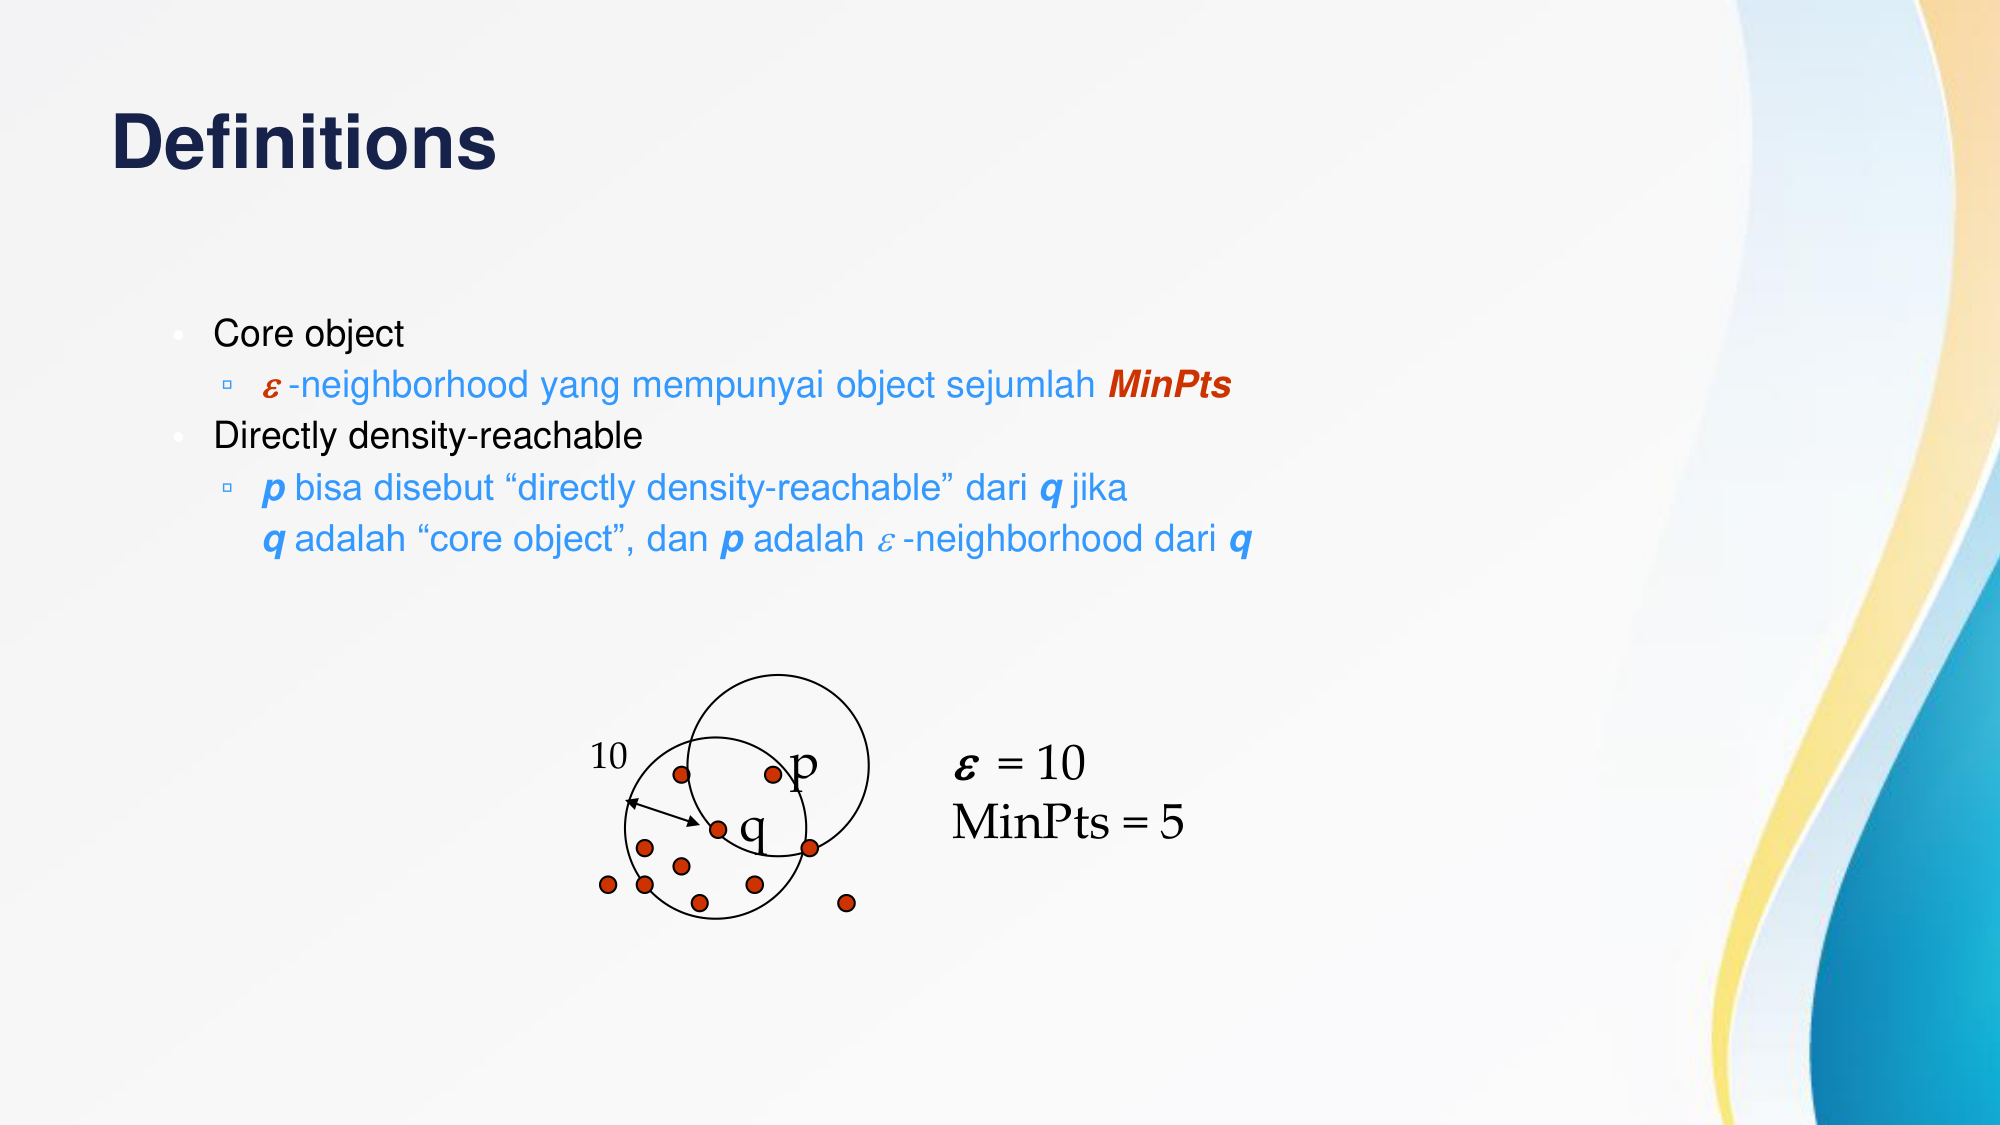
\includegraphics[width=\dimexpr\linewidth-1pt\relax]{images/gambar-6-2-14-dbscan-core-object.png}}
    \caption{Titik inti batas $\epsilon$ dan $MinPts$ \cite{ester1996}.}
    \label{fig:dbscan-core}
\end{minipage}
\hfill
\begin{minipage}[b]{0.48\textwidth}
    \centering
    \customfbox{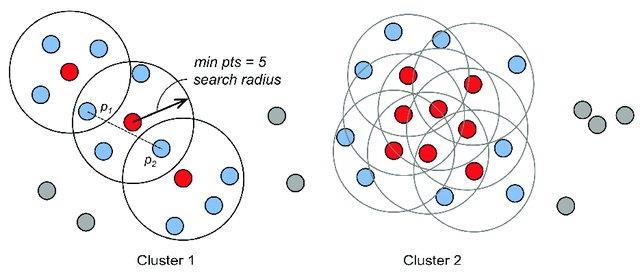
\includegraphics[width=\dimexpr\linewidth-1pt\relax]{images/gambar-6-2-15-dbscan-point-types.png}}
    \caption{Tiga tipe titik DBSCAN \cite{sander1998}.}
    \label{fig:dbscan-types}
\end{minipage}
\end{figure}

Penentuan parameter $\mathit{MinPts}$ mengikuti aturan praktis: untuk data 2 dimensi digunakan $\mathit{MinPts} = 4$ \cite{ester1996}, sedangkan untuk dimensi $D > 2$ disarankan $\mathit{MinPts} = 2 \times D$ \cite{sander1998}. Nilai $\epsilon$ ditentukan memakai grafik jarak k-tetangga terurut (sorted k-distance graph) dengan $k = \mathit{MinPts}$. Nilai $\epsilon$ optimal diambil pada titik kelokan kurva, seperti tampak pada Gambar~\ref{fig:dbscan-kdist}.

\begin{figure}[H]
\centering
\fbox{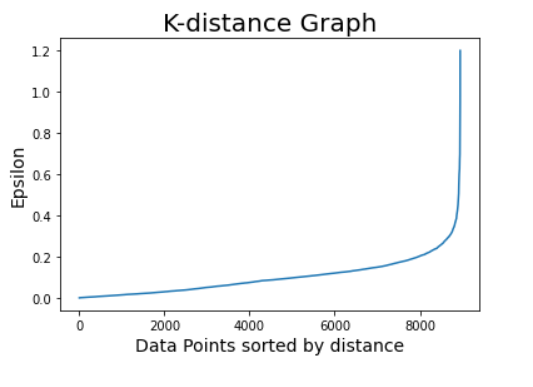
\includegraphics[width=0.45\textwidth]{images/gambar-6-2-16-dbscan-k-dist-graph.png}}
\caption{Grafik sorted k-distance untuk menentukan nilai $\epsilon$ optimal \cite{ester1996}.}
\label{fig:dbscan-kdist}
\end{figure}

\section{Association Rule Mining}
Association Rule Mining menemukan keterkaitan kemunculan bersama antar-item dalam basis data transaksi transaksi keranjang belanja (Market Basket Analysis) \cite{agrawal1993}. Contoh data transaksi belanja ditunjukkan pada Gambar~\ref{fig:assoc-trans}.

\begin{figure}[H]
\centering
\fbox{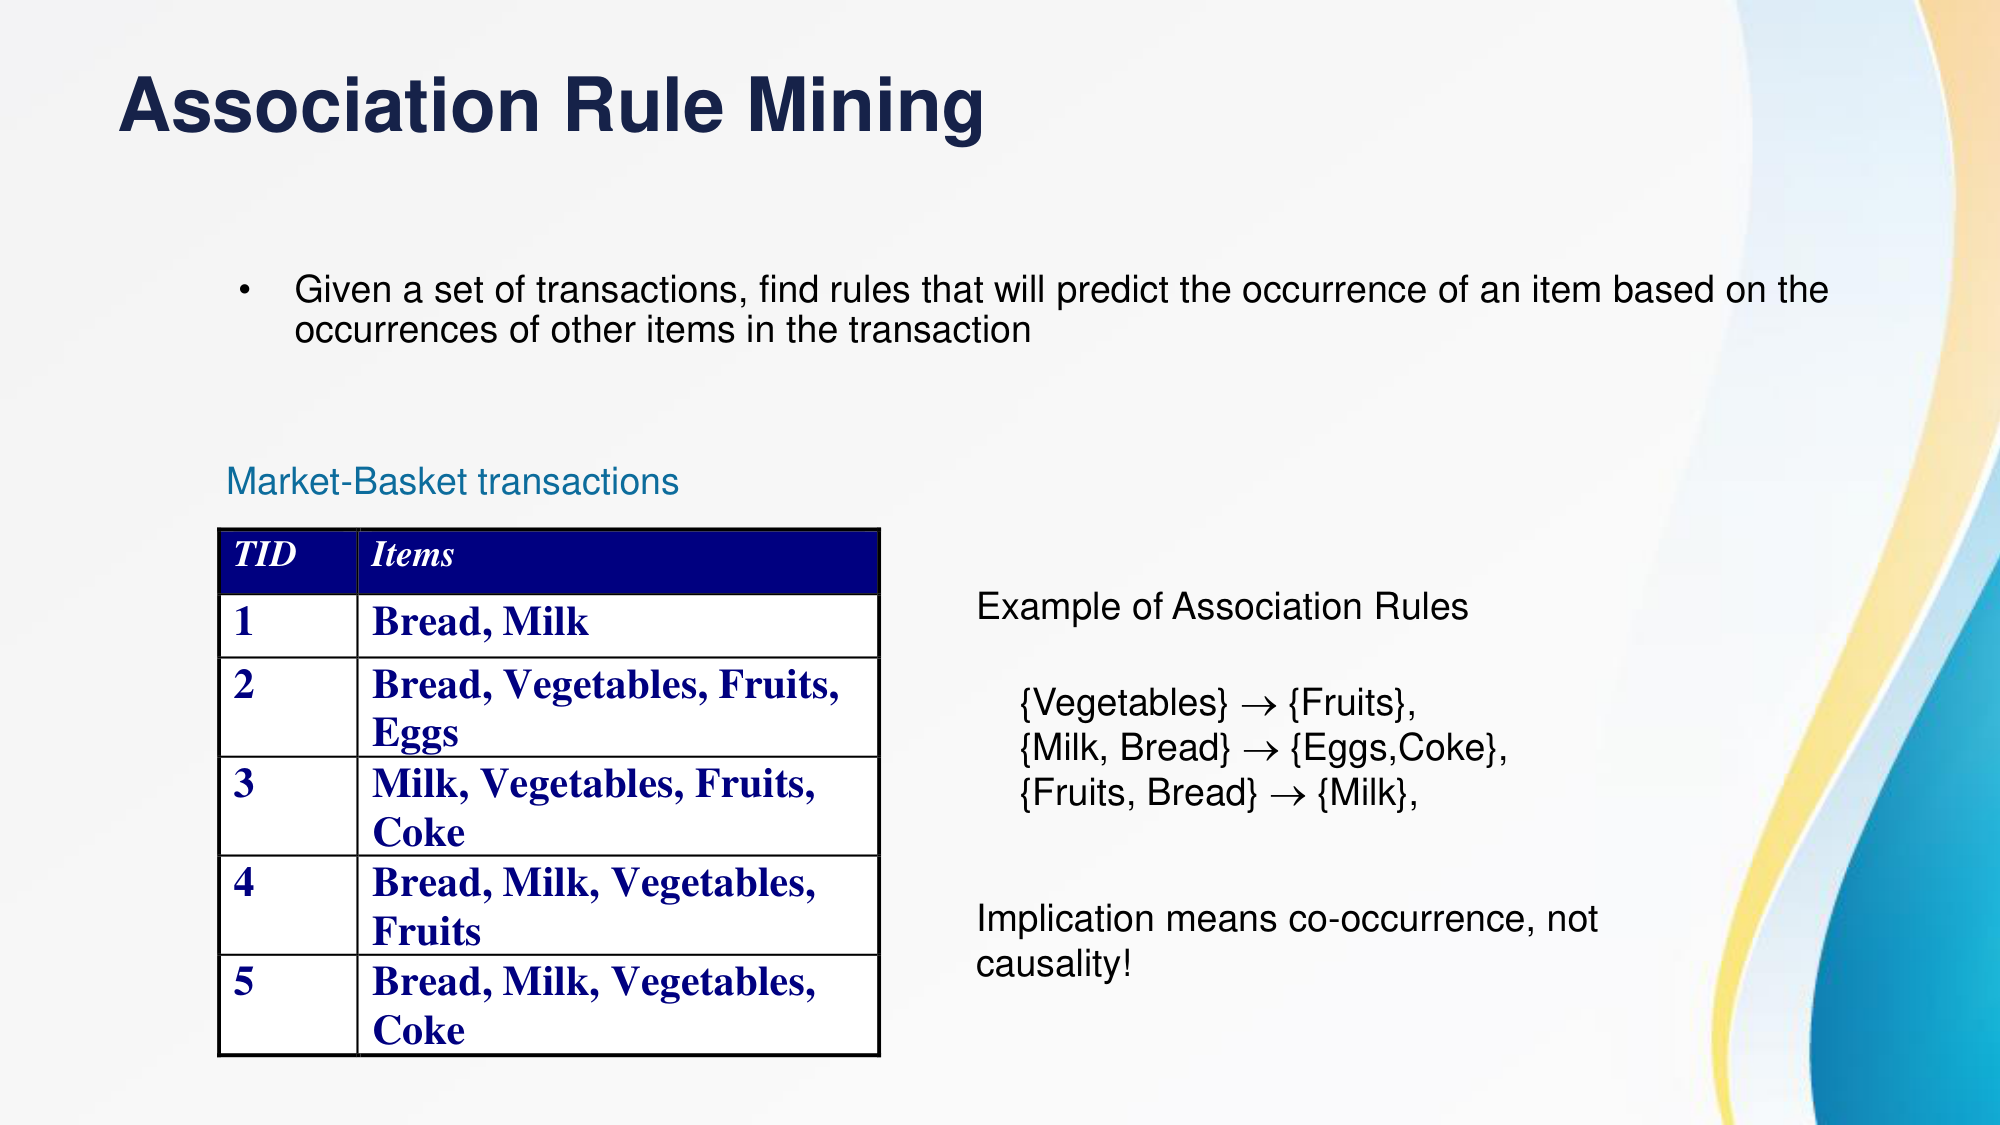
\includegraphics[width=0.48\textwidth]{images/gambar-6-2-17-association-rule-transactions.png}}
\caption{Contoh basis data transaksi keranjang belanja \cite{tan2019}.}
\label{fig:assoc-trans}
\end{figure}

Aturan asosiasi ditulis dalam bentuk implikasi logis:
\begin{equation}
X \rightarrow Y, \quad \text{dengan } X \cap Y = \emptyset
\end{equation}
dengan $X$ sebagai antecedent dan $Y$ sebagai consequent. Pernyataan ini menyatakan kecenderungan kemunculan bersama (co-occurrence), bukan hubungan sebab-akibat kausalitas.

Tiga metrik kualitas aturan asosiasi meliputi:
\begin{enumerate}[noitemsep, topsep=1pt, parsep=0.5pt]
    \item \textbf{Support ($s$):} Fraksi transaksi dalam database yang memuat kombinasi $X$ dan $Y$ bersamaan: $s(X \rightarrow Y) = \frac{\sigma(X \cup Y)}{|T|}$.
    \item \textbf{Confidence ($c$):} Peluang bersyarat kemunculan $Y$ pada transaksi yang memuat $X$: $c(X \rightarrow Y) = \frac{\sigma(X \cup Y)}{\sigma(X)}$.
    \item \textbf{Lift:} Kekuatan aturan terhadap asumsi saling bebas: $\mathit{Lift}(X \rightarrow Y) = \frac{c(X \rightarrow Y)}{s(Y)} = \frac{s(X \cup Y)}{s(X) \cdot s(Y)}$. Nilai $\mathit{Lift} > 1$ menandakan asosiasi positif, $\mathit{Lift} = 1$ independen, dan $\mathit{Lift} < 1$ substitutif.
\end{enumerate}

Pada basis data berisi lima transaksi: TID 1: $\{\text{Bread}, \text{Milk}\}$, TID 2: $\{\text{Bread}, \text{Vegetables}, \text{Fruits}, \text{Eggs}\}$, TID 3: $\{\text{Milk}, \text{Vegetables}, \text{Fruits}, \text{Coke}\}$, TID 4: $\{\text{Bread}, \text{Milk}, \text{Vegetables}, \text{Fruits}\}$, dan TID 5: $\{\text{Bread}, \text{Milk}, \text{Vegetables}, \text{Coke}\}$. Perhitungan untuk aturan $\{\text{Milk}, \text{Vegetables}\} \rightarrow \{\text{Fruits}\}$ menghasilkan $\text{Support} = 2/5 = 0{,}40$, $\text{Confidence} = 2/3 \approx 0{,}67$, dan $\mathit{Lift} = 0{,}40 / (0{,}60 \times 0{,}60) \approx 1{,}11$. Nilai $\mathit{Lift} > 1$ mengonfirmasi bahwa aturan ini memiliki asosiasi positif yang valid. Rincian metrik dan contoh perhitungannya ditampilkan pada Gambar~\ref{fig:assoc-metrics} dan Gambar~\ref{fig:assoc-calc}.

\begin{figure}[H]
\centering
\begin{minipage}[b]{0.48\textwidth}
    \centering
    \customfbox{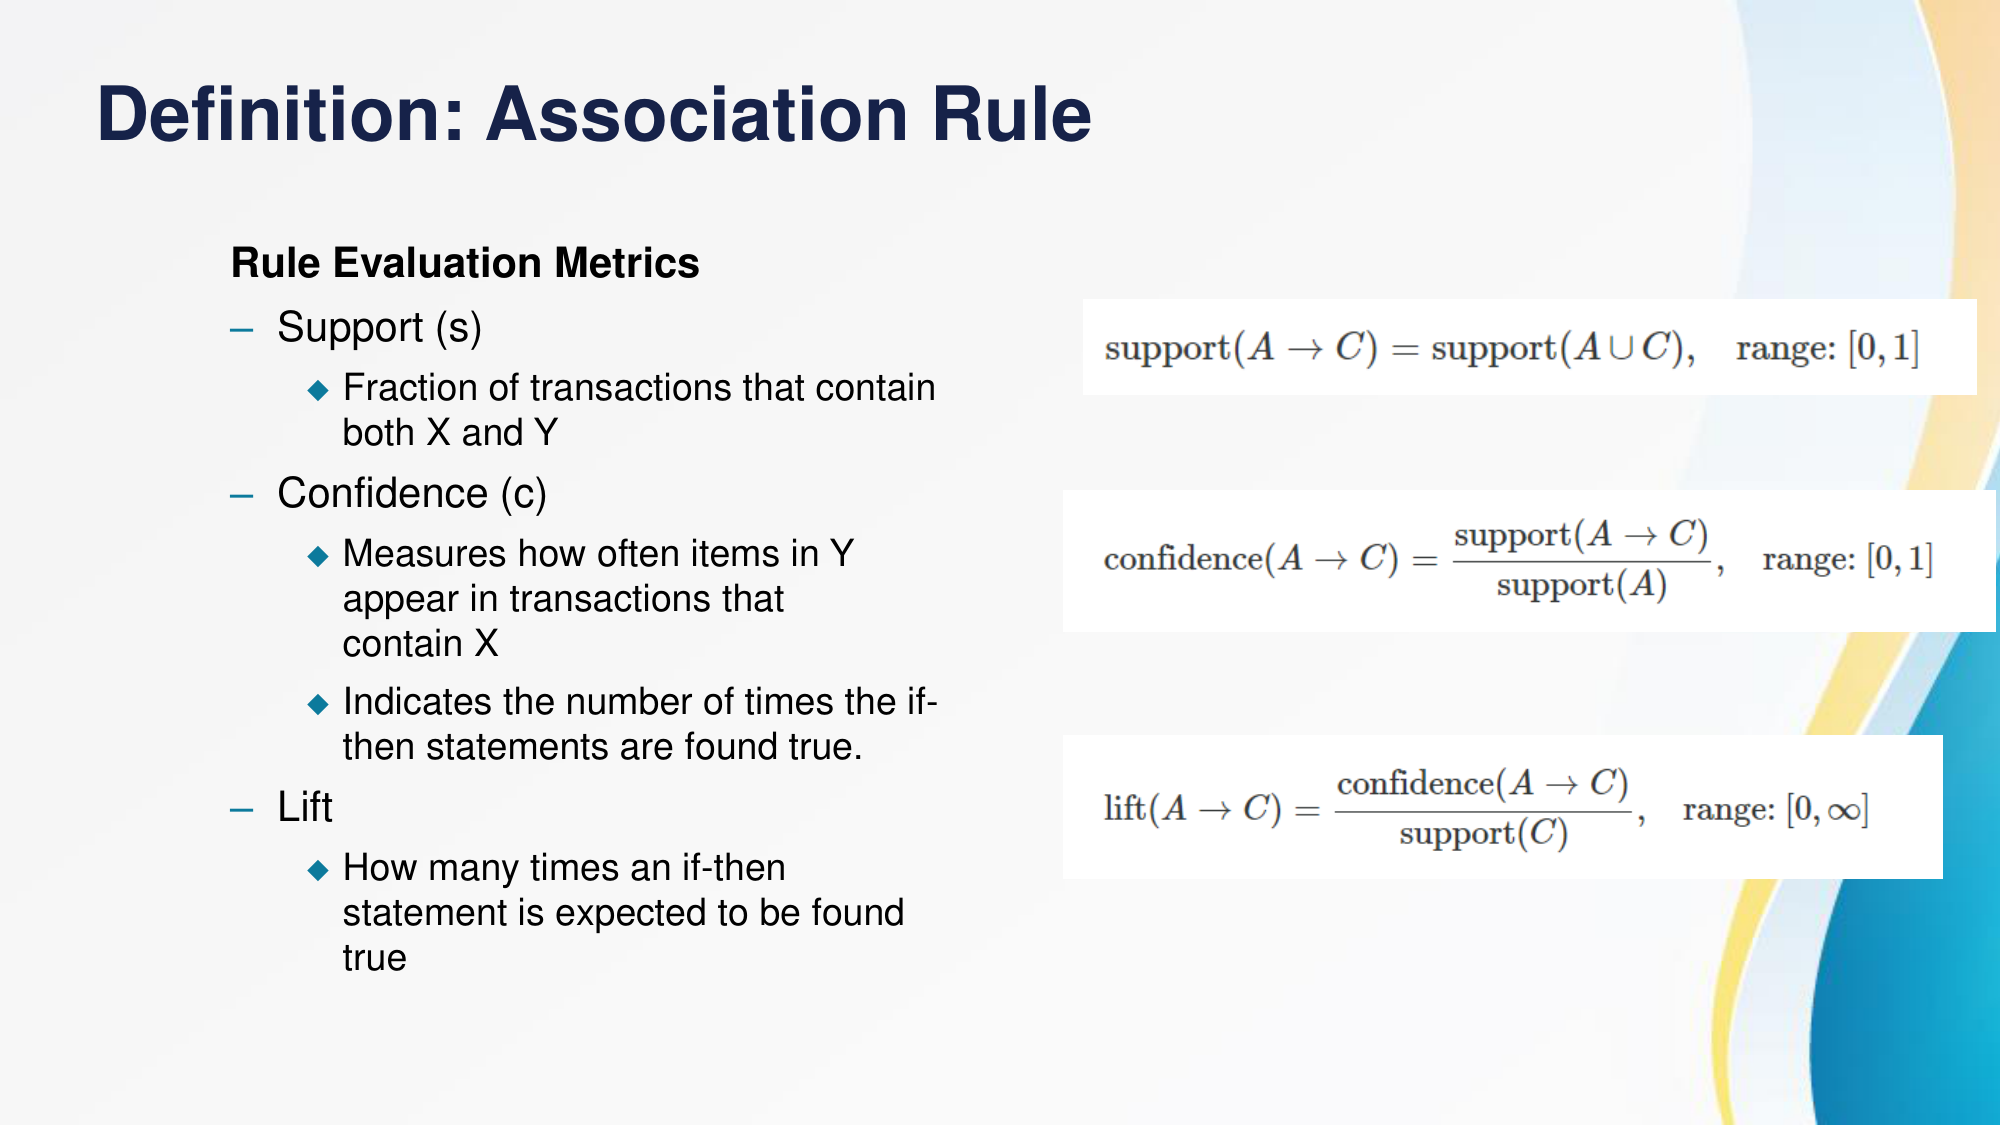
\includegraphics[width=\dimexpr\linewidth-1pt\relax]{images/gambar-6-2-17b-association-rule-metrics.png}}
    \caption{Metrik evaluasi aturan asosiasi \cite{tan2019}.}
    \label{fig:assoc-metrics}
\end{minipage}
\hfill
\begin{minipage}[b]{0.48\textwidth}
    \centering
    \customfbox{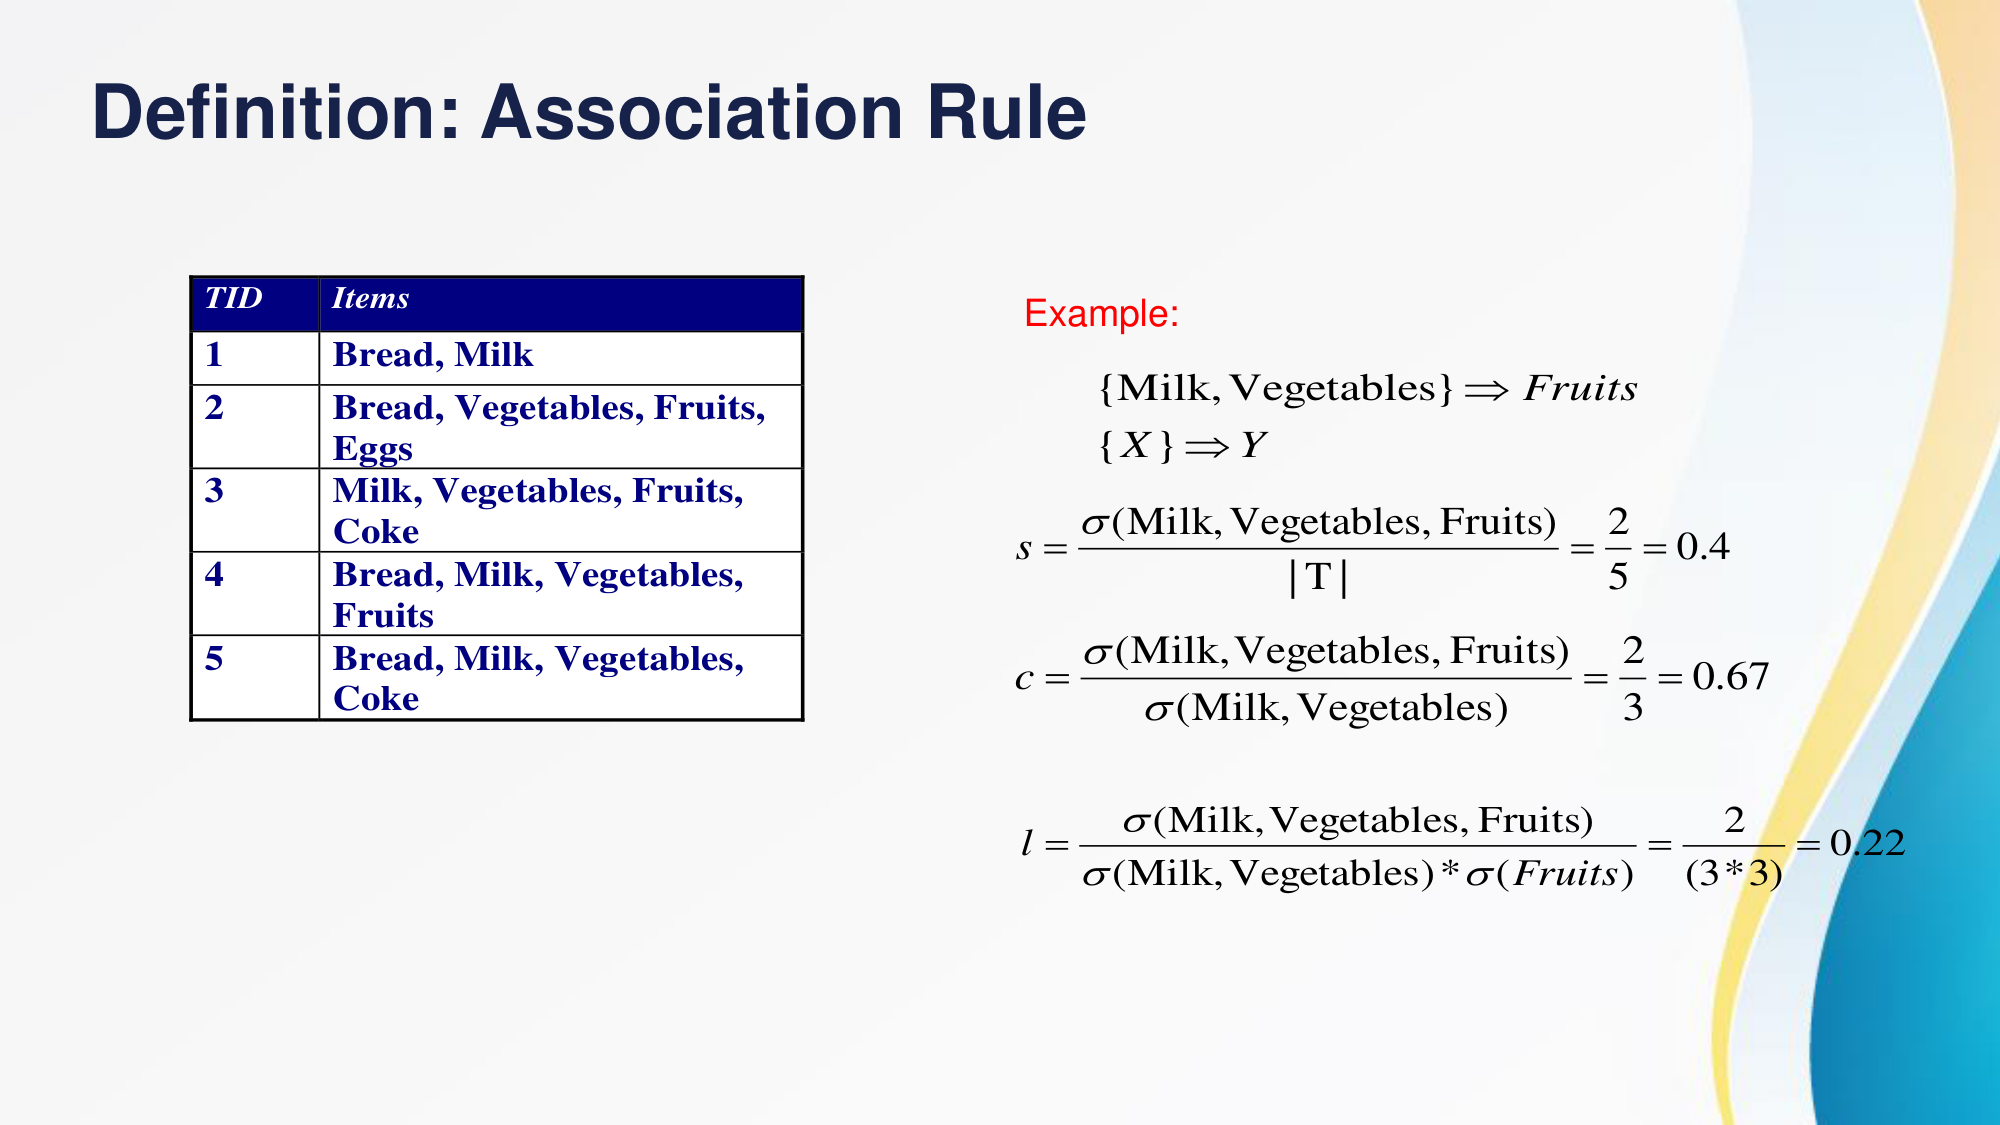
\includegraphics[width=\dimexpr\linewidth-1pt\relax]{images/gambar-6-2-17c-association-rule-example.png}}
    \caption{Langkah perhitungan metrik \cite{tan2019}.}
    \label{fig:assoc-calc}
\end{minipage}
\end{figure}

\section{Algoritma Apriori}
Untuk basis data dengan $d$ item berbeda, ruang pencarian memuat $2^d - 1$ kemungkinan kombinasi itemset. Algoritma Apriori diperkenalkan oleh Rakesh Agrawal dan Ramakrishnan Srikant pada tahun 1994 untuk menekan ledakan kombinatorial ini \cite{agrawal1994}. Prinsip Apriori berpegang pada sifat anti-monoton nilai support: jika suatu itemset bersifat frequent, maka seluruh himpunan bagiannya (subset) pasti frequent. Sebaliknya, jika suatu itemset tidak frequent, maka seluruh superset yang memuatnya dipastikan tidak frequent dan langsung dipangkas (lattice pruning), seperti diilustrasikan pada Gambar~\ref{fig:apriori-principle} dan Gambar~\ref{fig:apriori-lattice}.

\begin{figure}[H]
\centering
\begin{minipage}[b]{0.46\textwidth}
    \centering
    \customfbox{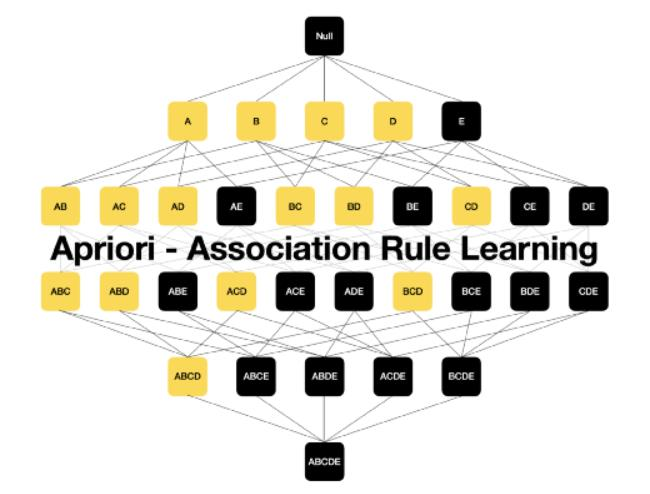
\includegraphics[width=\dimexpr\linewidth-1pt\relax]{images/gambar-6-2-18-apriori-principle.png}}
    \caption{Prinsip Apriori pada support \cite{agrawal1994}.}
    \label{fig:apriori-principle}
\end{minipage}
\hfill
\begin{minipage}[b]{0.50\textwidth}
    \centering
    \customfbox{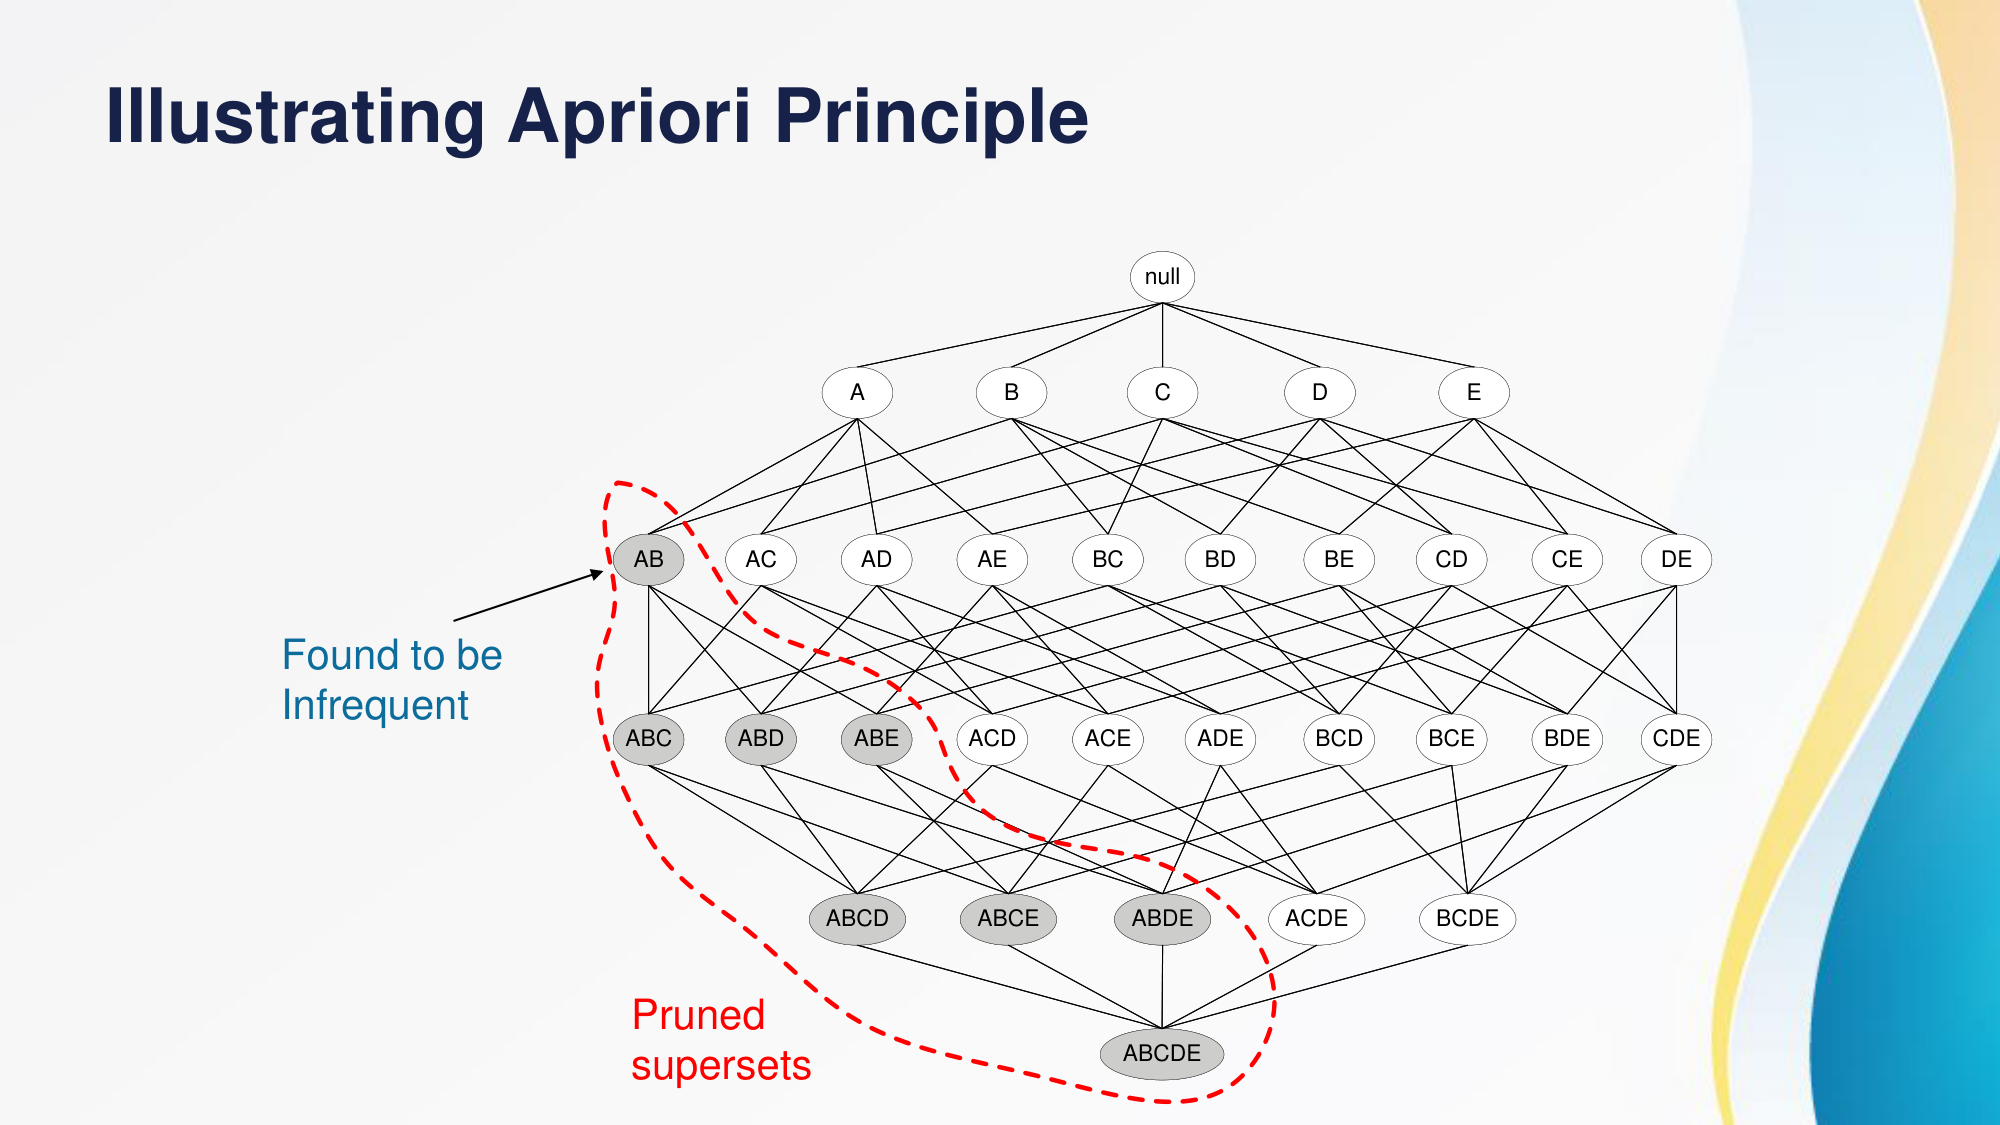
\includegraphics[width=\dimexpr\linewidth-1pt\relax]{images/gambar-6-2-20-apriori-lattice-superset.png}}
    \caption{Pemangkasan ruang superset \cite{tan2019}.}
    \label{fig:apriori-lattice}
\end{minipage}
\end{figure}

Alur kerja iteratif algoritma Apriori menghasilkan frequent 1-itemset ($L_1$), lalu membangkitkan kandidat $C_{k+1}$ melalui langkah penggabungan (join), memangkas kandidat yang memuat subset tidak frequent (prune), dan memindai database untuk menyaring $L_{k+1}$, seperti tampak pada Gambar~\ref{fig:apriori-workflow}.

\begin{figure}[H]
\centering
\fbox{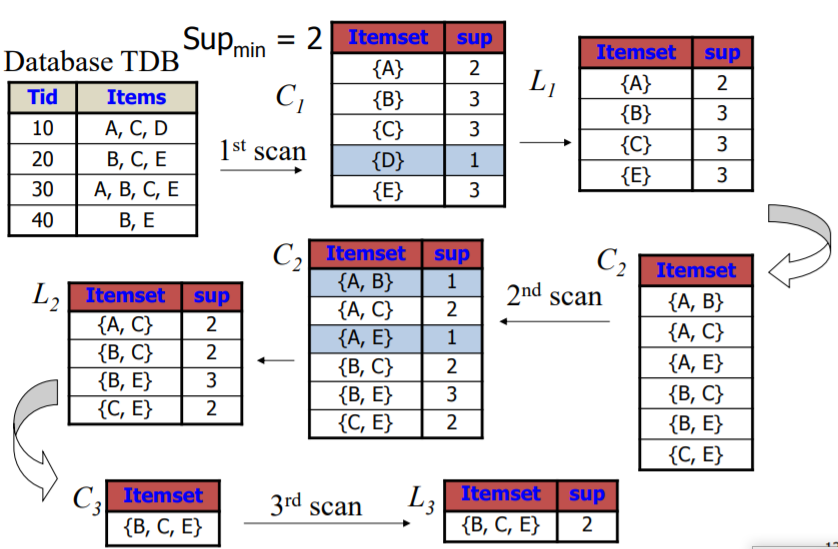
\includegraphics[width=0.50\textwidth]{images/gambar-6-2-19-apriori-lattice-pruning.png}}
\caption{Alur kerja algoritma Apriori: pembangkitan kandidat dan penyaringan bertahap \cite{agrawal1994}.}
\label{fig:apriori-workflow}
\end{figure}

\clearpage

\chapter{Alat dan Bahan}

Sesuai Modul Pertemuan 6 Praktikum Penambangan Data, alat dan bahan yang digunakan dalam praktikum ini meliputi:

\vspace{0.2cm}
\noindent\textbf{A. Perangkat Keras}
\begin{enumerate}[noitemsep, topsep=2pt, parsep=1pt]
    \item Komputer jinjing (laptop) dengan kapasitas memori minimal 4 GB RAM (direkomendasikan 8 GB atau lebih).
    \item Koneksi internet yang stabil untuk mengakses lingkungan komputasi daring dan mengunduh berkas dataset.
\end{enumerate}

\vspace{0.2cm}
\noindent\textbf{B. Perangkat Lunak}
\begin{enumerate}[noitemsep, topsep=2pt, parsep=1pt]
    \item Sistem operasi modern (Windows, macOS, atau Linux).
    \item Peramban web (Google Chrome, Mozilla Firefox, atau Microsoft Edge).
    \item Lingkungan pengembangan interaktif Python: Google Colaboratory dan Jupyter Notebook lokal.
    \item Bahasa pemrograman Python versi 3.8 ke atas \cite{python-docs}.
    \item Pustaka pemrograman Python:
    \begin{itemize}[noitemsep, topsep=1pt, parsep=0.5pt]
        \item \texttt{pandas} dan \texttt{numpy} untuk manipulasi data tabular dan operasi matriks numerik \cite{pandas-docs,numpy-docs}.
        \item \texttt{matplotlib.pyplot} dan \texttt{seaborn} untuk pembuatan grafik 2 dimensi \cite{matplotlib-docs,seaborn-docs}.
        \item \texttt{plotly.express} untuk pembuatan visualisasi sebaran klaster interaktif 3 dimensi \cite{plotly-docs}.
        \item \texttt{scikit-learn} untuk standarisasi skala (\texttt{StandardScaler}), pengkodean label (\texttt{LabelEncoder}), pemodelan \texttt{KMeans}, dan metrik \texttt{silhouette\_score} \cite{sklearn-clustering,sklearn-scaler,sklearn-encoder}.
        \item \texttt{scikit-learn-extra} untuk implementasi algoritma \texttt{KMedoids} \cite{sklearn-extra-kmedoids}.
        \item \texttt{kneed} (\texttt{KneeLocator}) untuk mendeteksi koordinat titik siku kurva secara otomatis \cite{kneed-docs}.
    \end{itemize}
\end{enumerate}


\clearpage

\chapter[\texorpdfstring{\tocboldsection{Hasil dan Pembahasan}}{Hasil dan Pembahasan}]{Hasil dan Pembahasan}

\section{Percobaan Latihan Praktikum}
Percobaan latihan praktikum mengimplementasikan segmentasi nasabah kartu kredit memakai \textit{Credit Card Dataset for Clustering} (\texttt{CC GENERAL.csv}) \cite{kaggle-ccdata}. Seluruh tahapan eksperimen latihan dan tugas pada laporan ini telah diimplementasikan dalam notebook yang dapat diakses dan dijalankan langsung melalui Google Colab pada tautan berikut:

\begin{center}
\href{https://colab.research.google.com/github/hafidzrizqullahprasetya/PPD/blob/main/pertemuan-6/praktikum-6-clustering.ipynb}{\textcolor{blue}{\url{https://colab.research.google.com/github/hafidzrizqullahprasetya/PPD/blob/main/pertemuan-6/praktikum-6-clustering.ipynb}}} \cite{colab-notebook}
\end{center}

Tangkapan layar pada setiap tahapan disiapkan memakai slot gambar acuan untuk penyesuaian mandiri.

\subsection{Persiapan dan Impor Pustaka}
Tahap awal menginstal pustaka tambahan `scikit-learn-extra` dan `kneed`, lalu mengimpor pustaka utama untuk manipulasi data, standarisasi, pemodelan klaster, dan visualisasi.

\begin{lstlisting}[style=pythonstyle,caption={Impor pustaka praktikum klasterisasi.}]
import numpy as np
import pandas as pd
import matplotlib.pyplot as plt
import seaborn as sns
import plotly.express as px

from sklearn.preprocessing import StandardScaler
from sklearn.cluster import KMeans
from sklearn.metrics import silhouette_samples, silhouette_score
\end{lstlisting}

\begin{figure}[H]
\centering
\customfbox{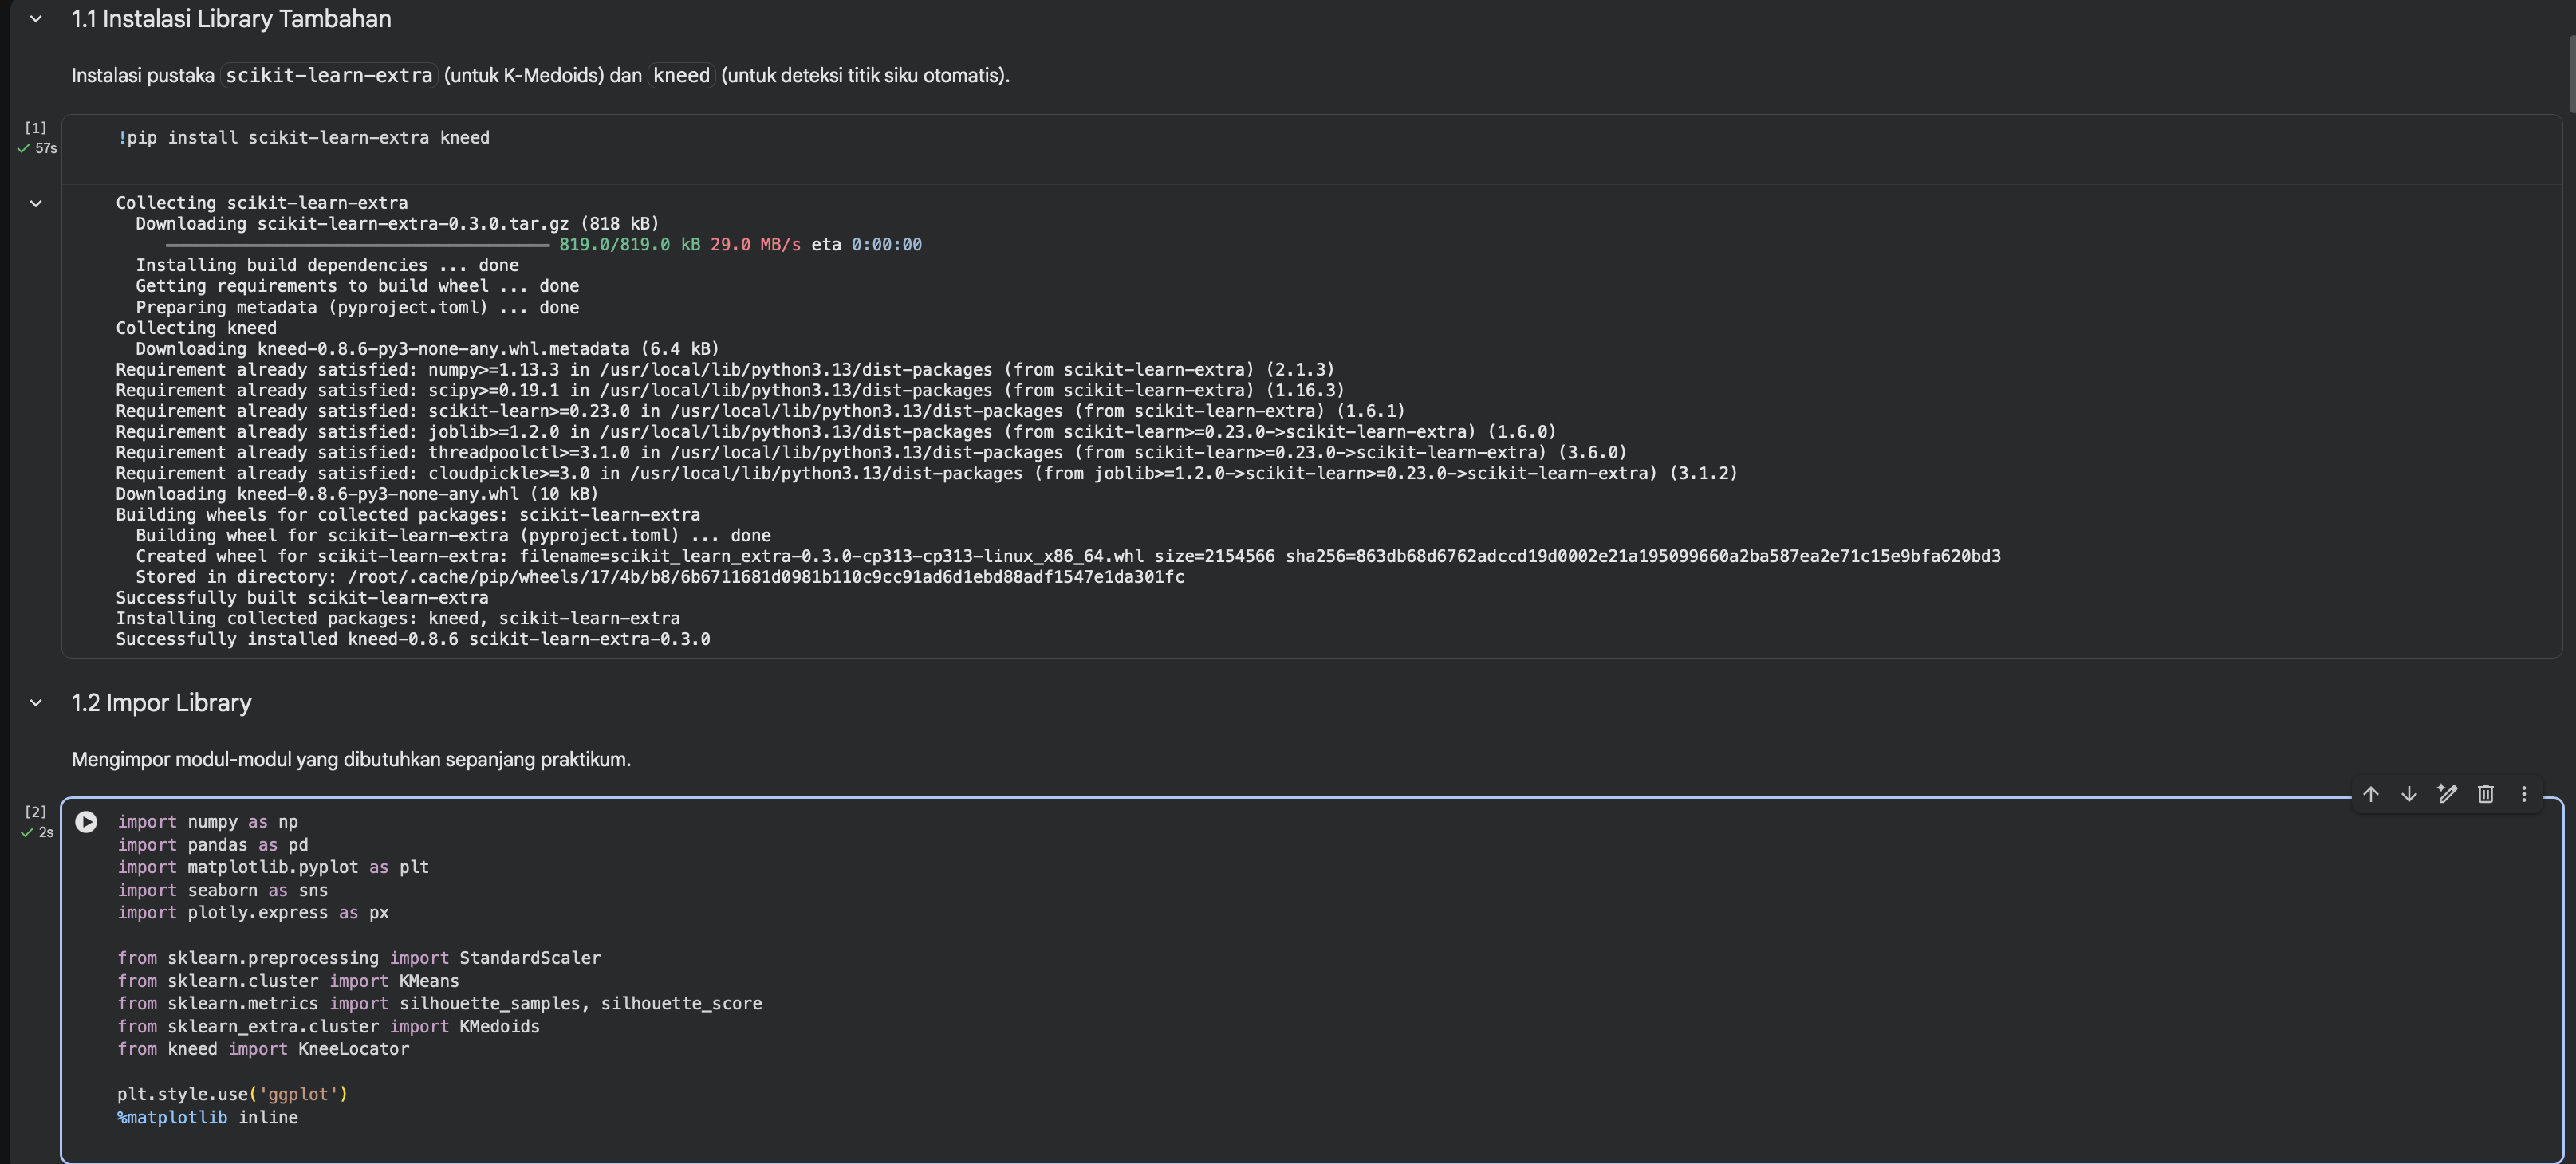
\includegraphics[width=0.9\textwidth]{images/ss-01-import-pustaka.png}}
\caption{Tangkapan layar impor pustaka utama pada Google Colab.}
\label{fig:ss-import-pustaka}
\end{figure}

\subsection{Membaca dan Memuat Informasi Dataset}
Dataset dibaca langsung dari tautan repositori daring menggunakan pandas. Dataset memuat 8.950 baris observasi dan 18 kolom fitur.

\begin{lstlisting}[style=pythonstyle,caption={Membaca dataset kartu kredit.}]
url = ('https://raw.githubusercontent.com/ganjar87/'
       'data_science_practice/main/CC%20GENERAL.csv')
df = pd.read_csv(url)
print("Dimensi dataset:", df.shape)
df.head()
\end{lstlisting}

\begin{figure}[H]
\centering
\customfbox{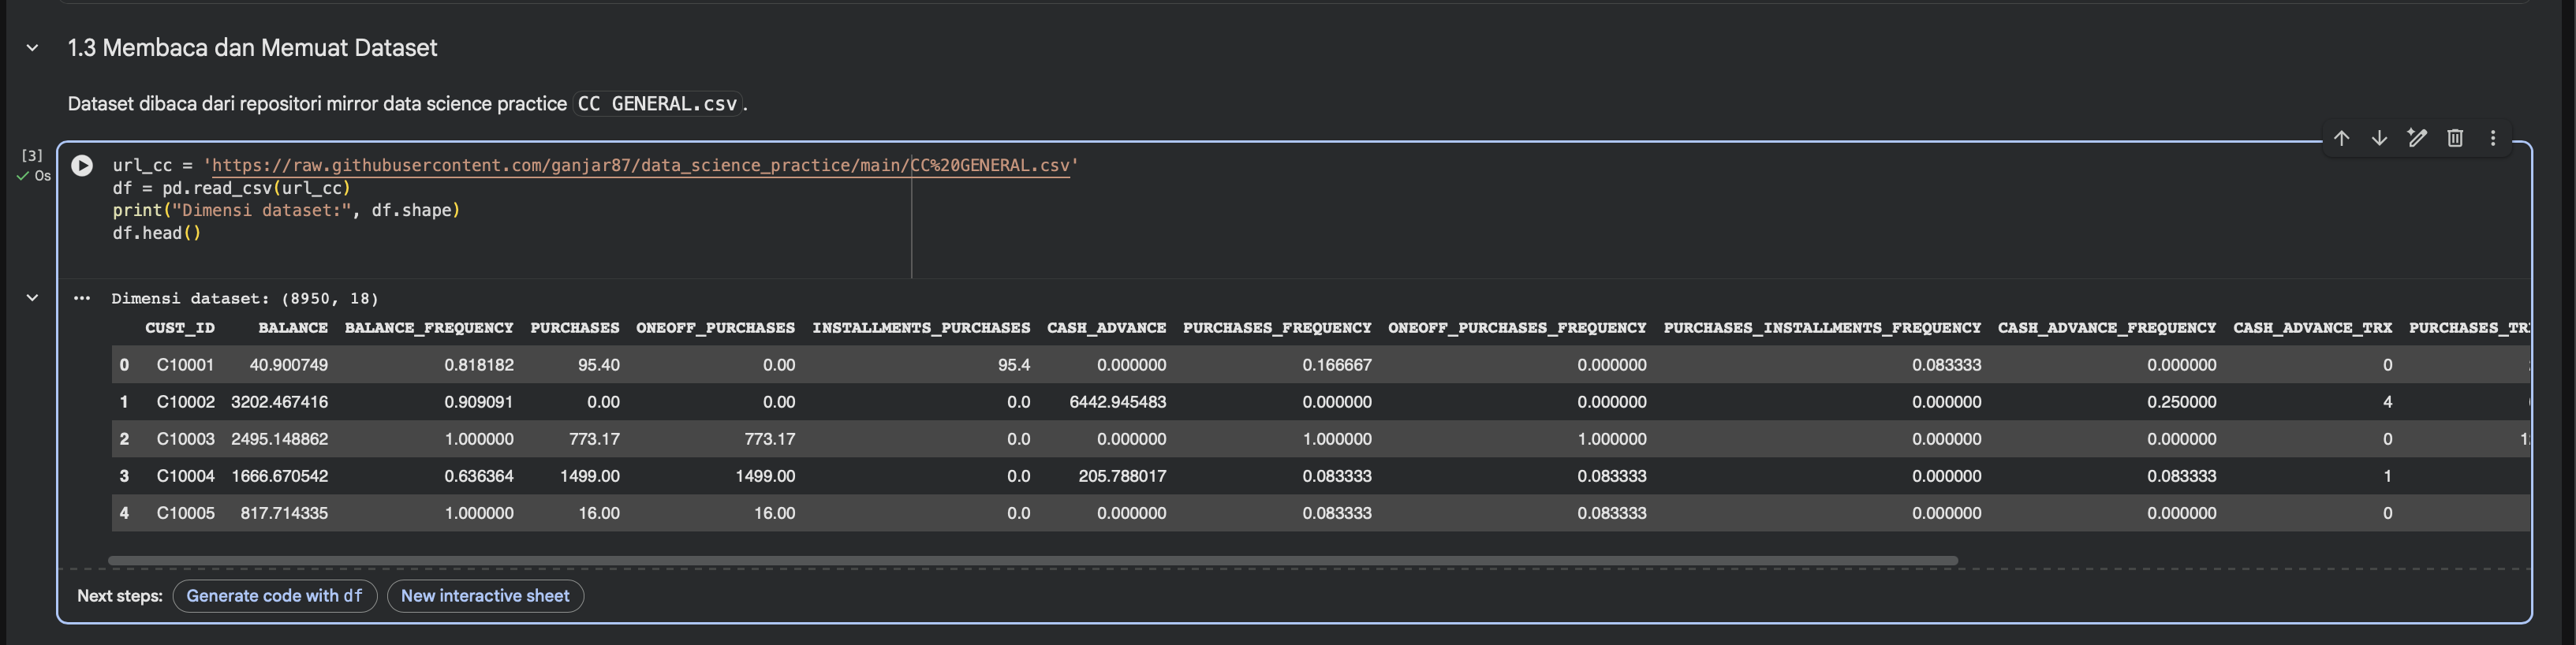
\includegraphics[width=0.9\textwidth]{images/ss-02-baca-dataset.png}}
\caption{Tangkapan layar pembacaan data dan lima baris pertama CC GENERAL.csv.}
\label{fig:ss-baca-dataset}
\end{figure}

Saya memeriksa struktur tipe data dan sebaran ringkasan statistik memakai \texttt{df.info()} dan \texttt{df.describe().T}. Dari pemeriksaan ini, 14 fitur bertipe \texttt{float64}, 3 fitur bertipe \texttt{int64}, dan 1 fitur teks yaitu \texttt{CUST\_ID}.

\begin{lstlisting}[style=pythonstyle,caption={Pemeriksaan tipe data dan statistik deskriptif.}]
df.info()
df.describe().T
\end{lstlisting}

\begin{figure}[H]
\centering
\customfbox{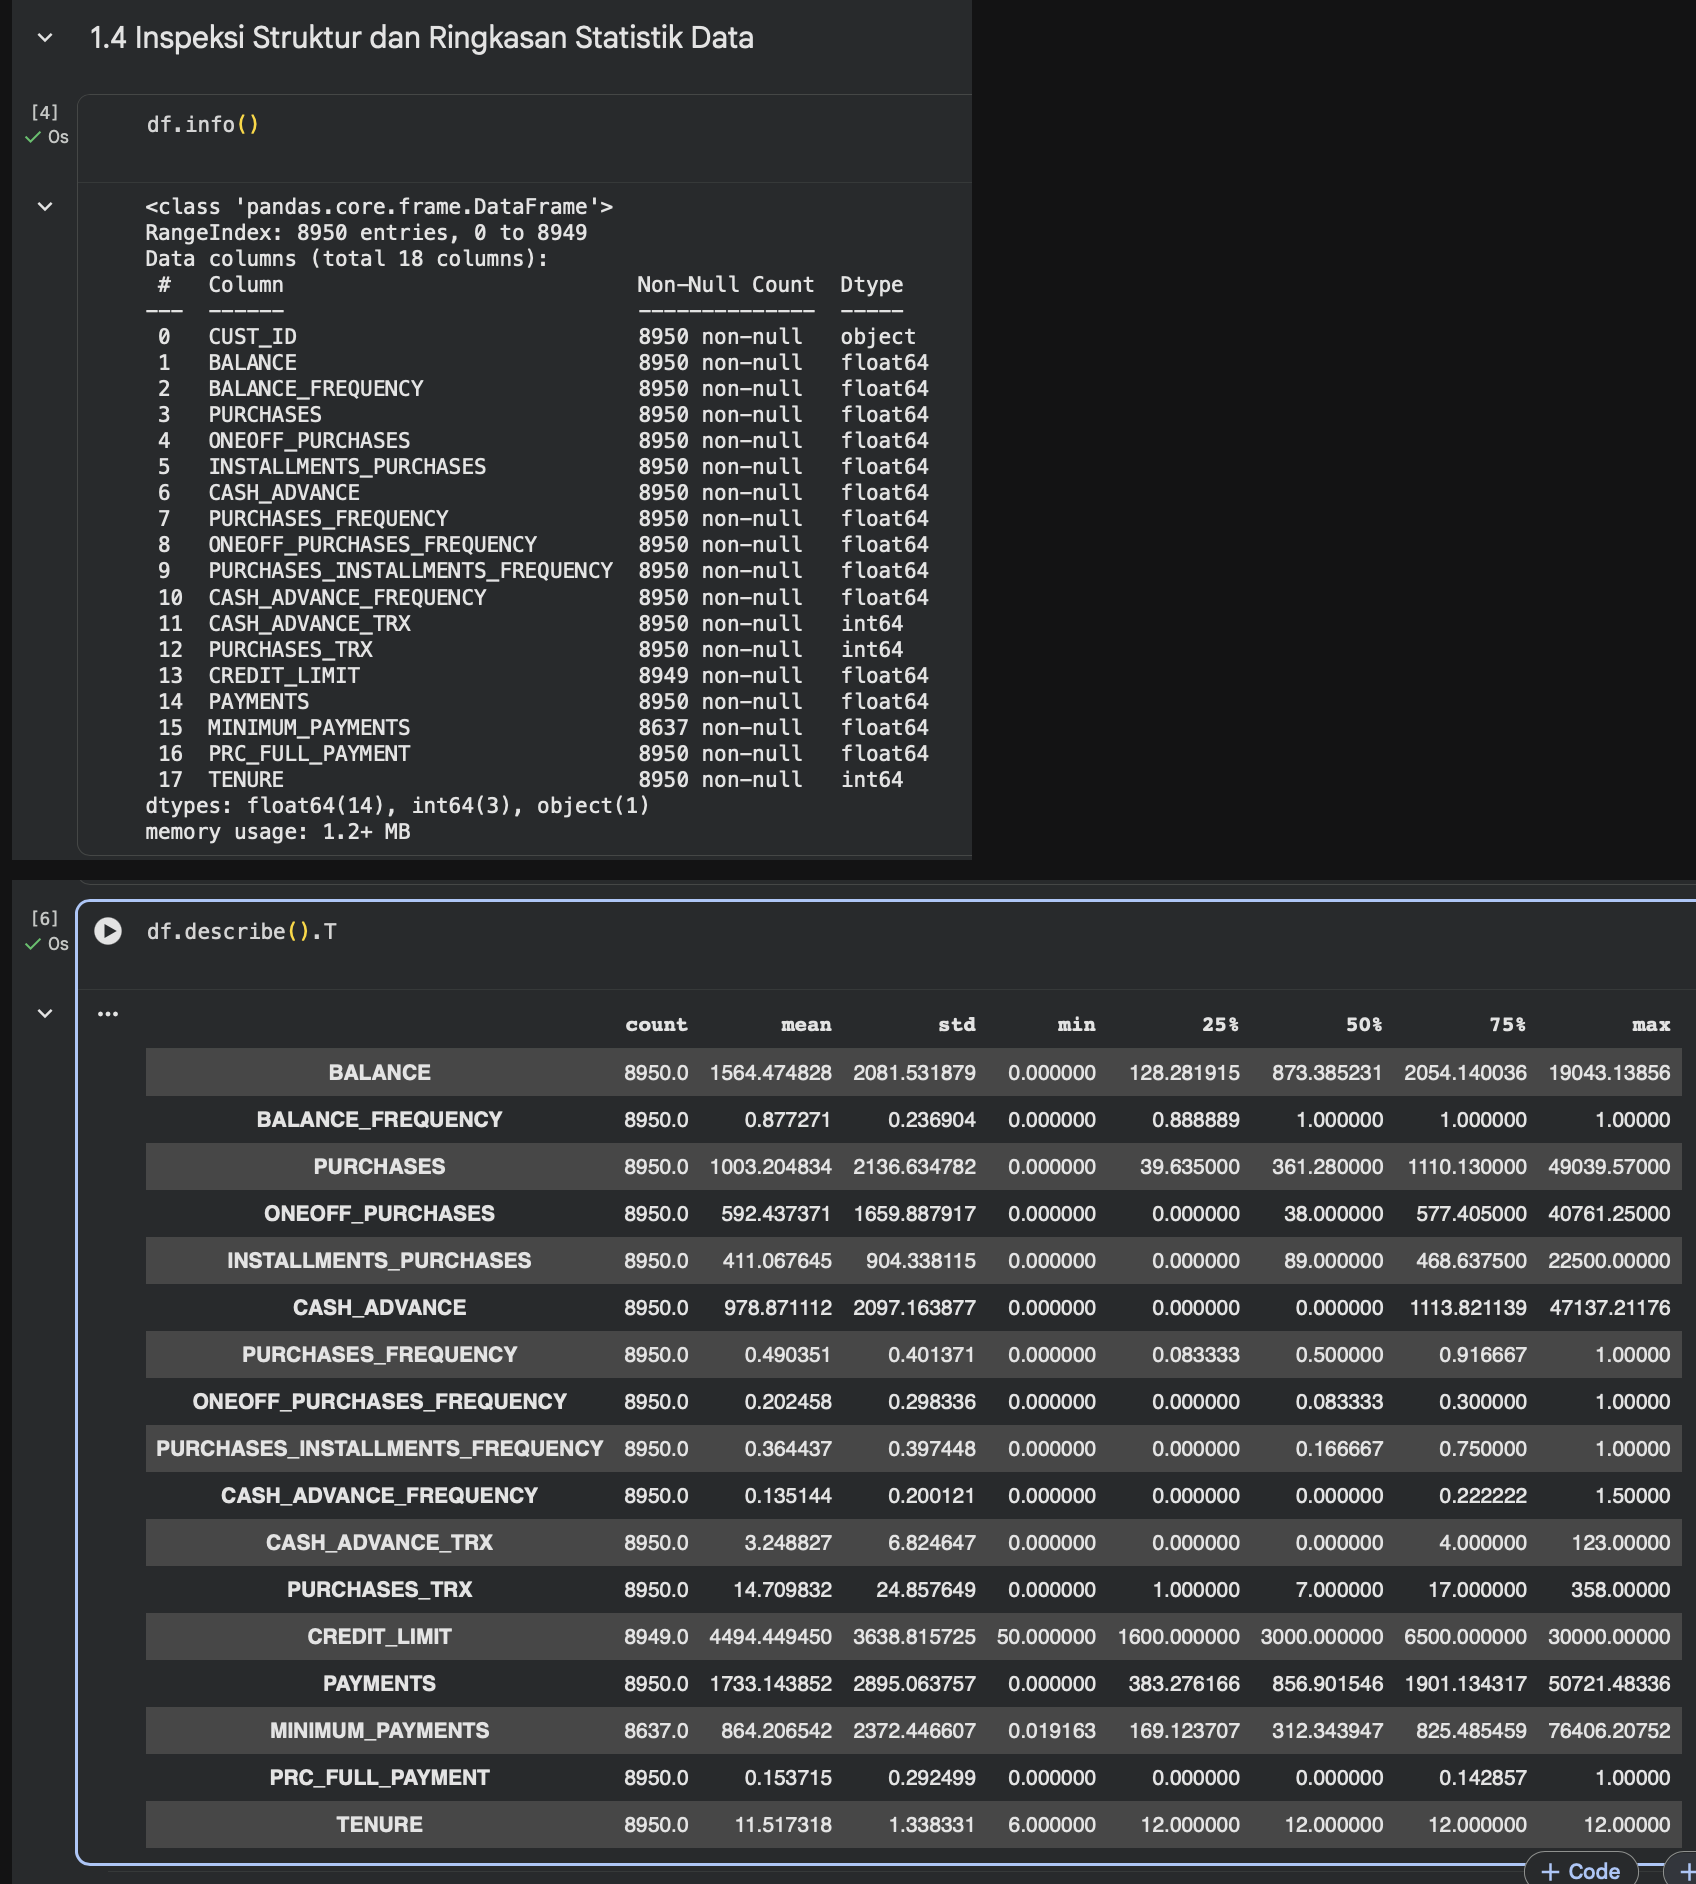
\includegraphics[width=0.85\textwidth]{images/ss-03-struktur-dataset.png}}
\caption{Tangkapan layar struktur tipe data dan ringkasan statistik deskriptif.}
\label{fig:ss-struktur-dataset}
\end{figure}

Korelasi Pearson dihitung untuk mengenali hubungan antar-variabel numerik. Fitur \texttt{PURCHASES} memiliki korelasi linear tinggi dengan \texttt{ONEOFF\_PURCHASES} ($r = 0{,}917$) dan berkorelasi moderat dengan \texttt{PAYMENTS} ($r = 0{,}603$).

\begin{lstlisting}[style=pythonstyle,caption={Pemeriksaan matriks korelasi antar-fitur.}]
df.corr(numeric_only=True)
\end{lstlisting}

\begin{figure}[H]
\centering
\customfbox{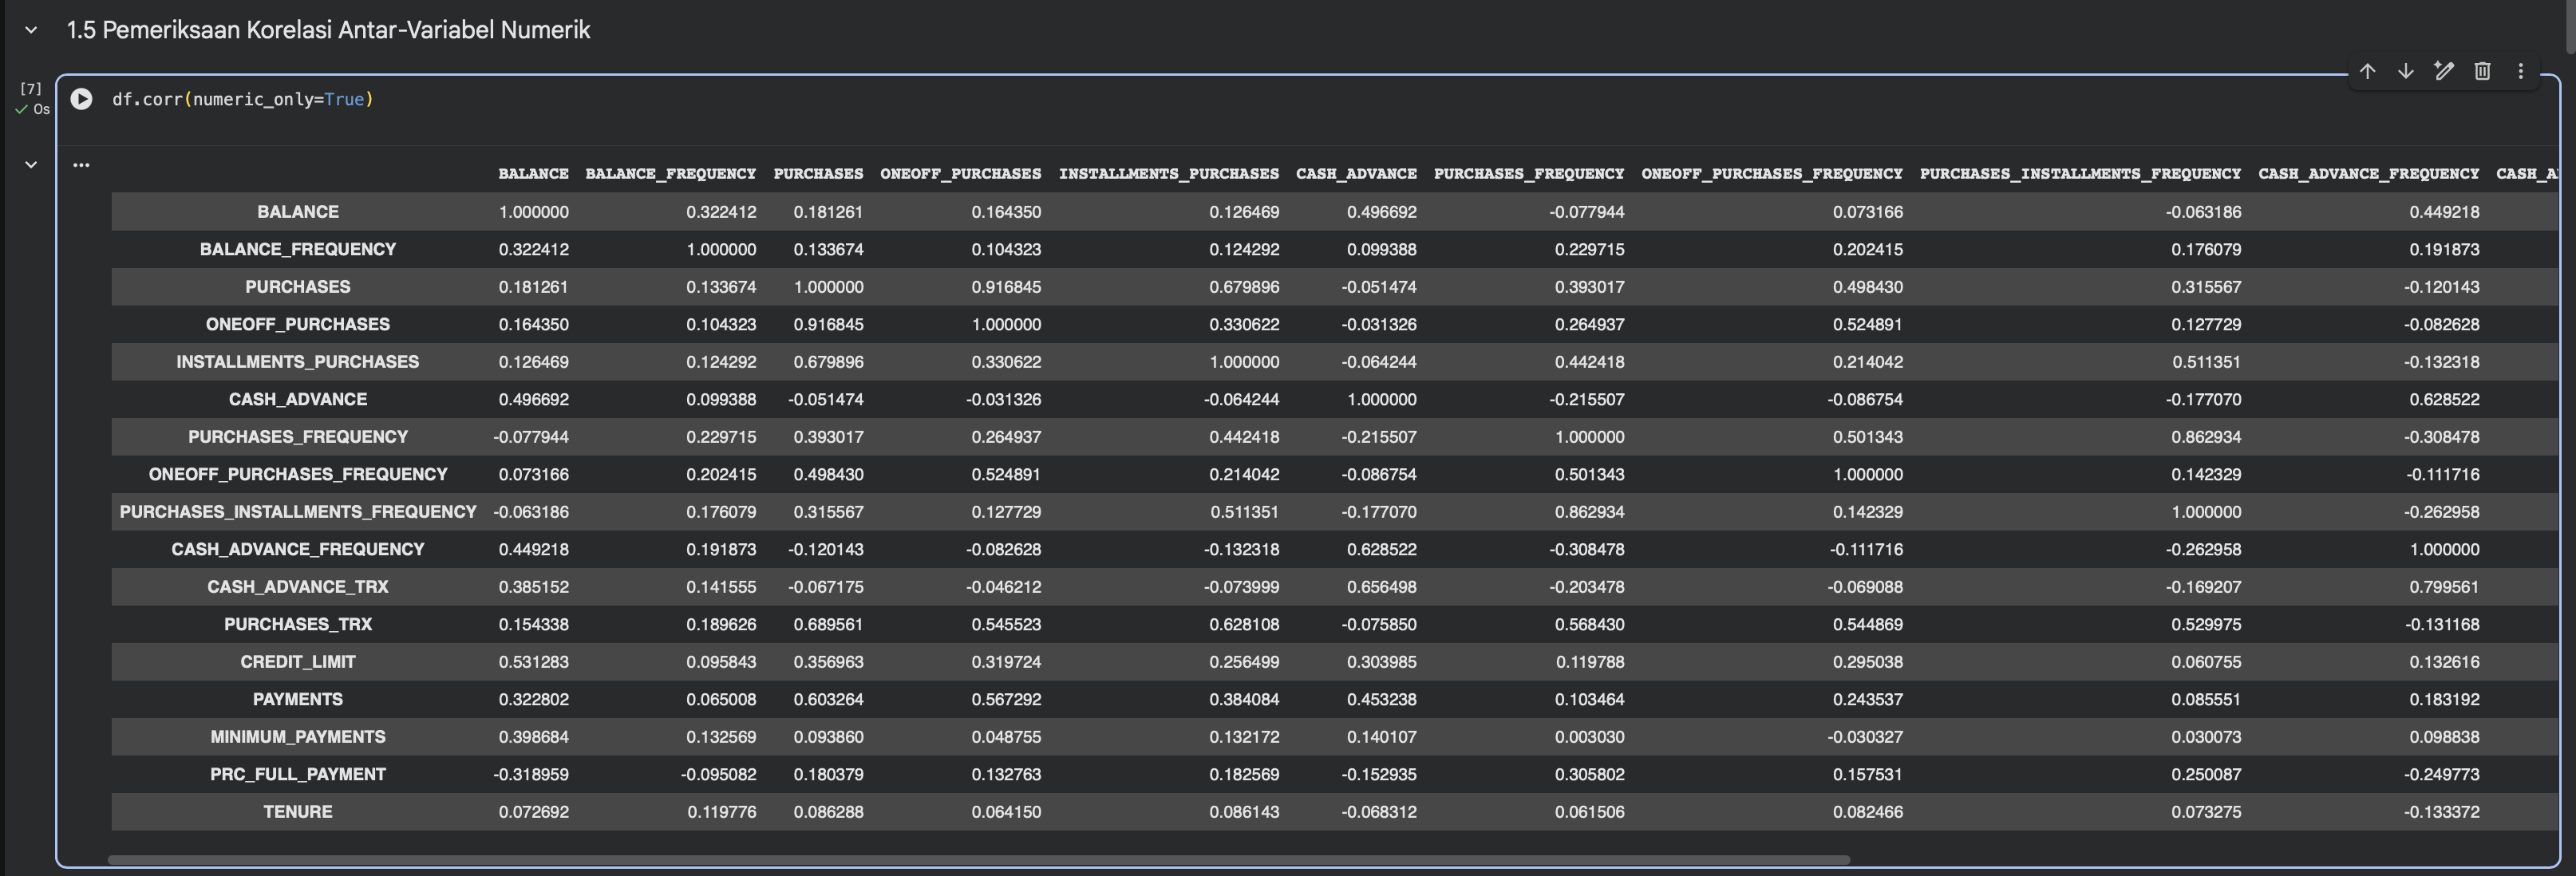
\includegraphics[width=0.9\textwidth]{images/ss-04-korelasi.png}}
\caption{Tangkapan layar matriks korelasi antar-variabel numerik.}
\label{fig:ss-korelasi}
\end{figure}

\subsection{Pembersihan Data (Data Cleaning)}
Kolom \texttt{CUST\_ID} dihapus karena hanya berupa kode pengenal nasabah yang tidak memiliki makna jarak geometris dalam klasterisasi.

\begin{lstlisting}[style=pythonstyle,caption={Menghapus kolom CUST\_ID.}]
df_new = df.drop('CUST_ID', axis=1)
df_new.head()
\end{lstlisting}

\begin{figure}[H]
\centering
\customfbox{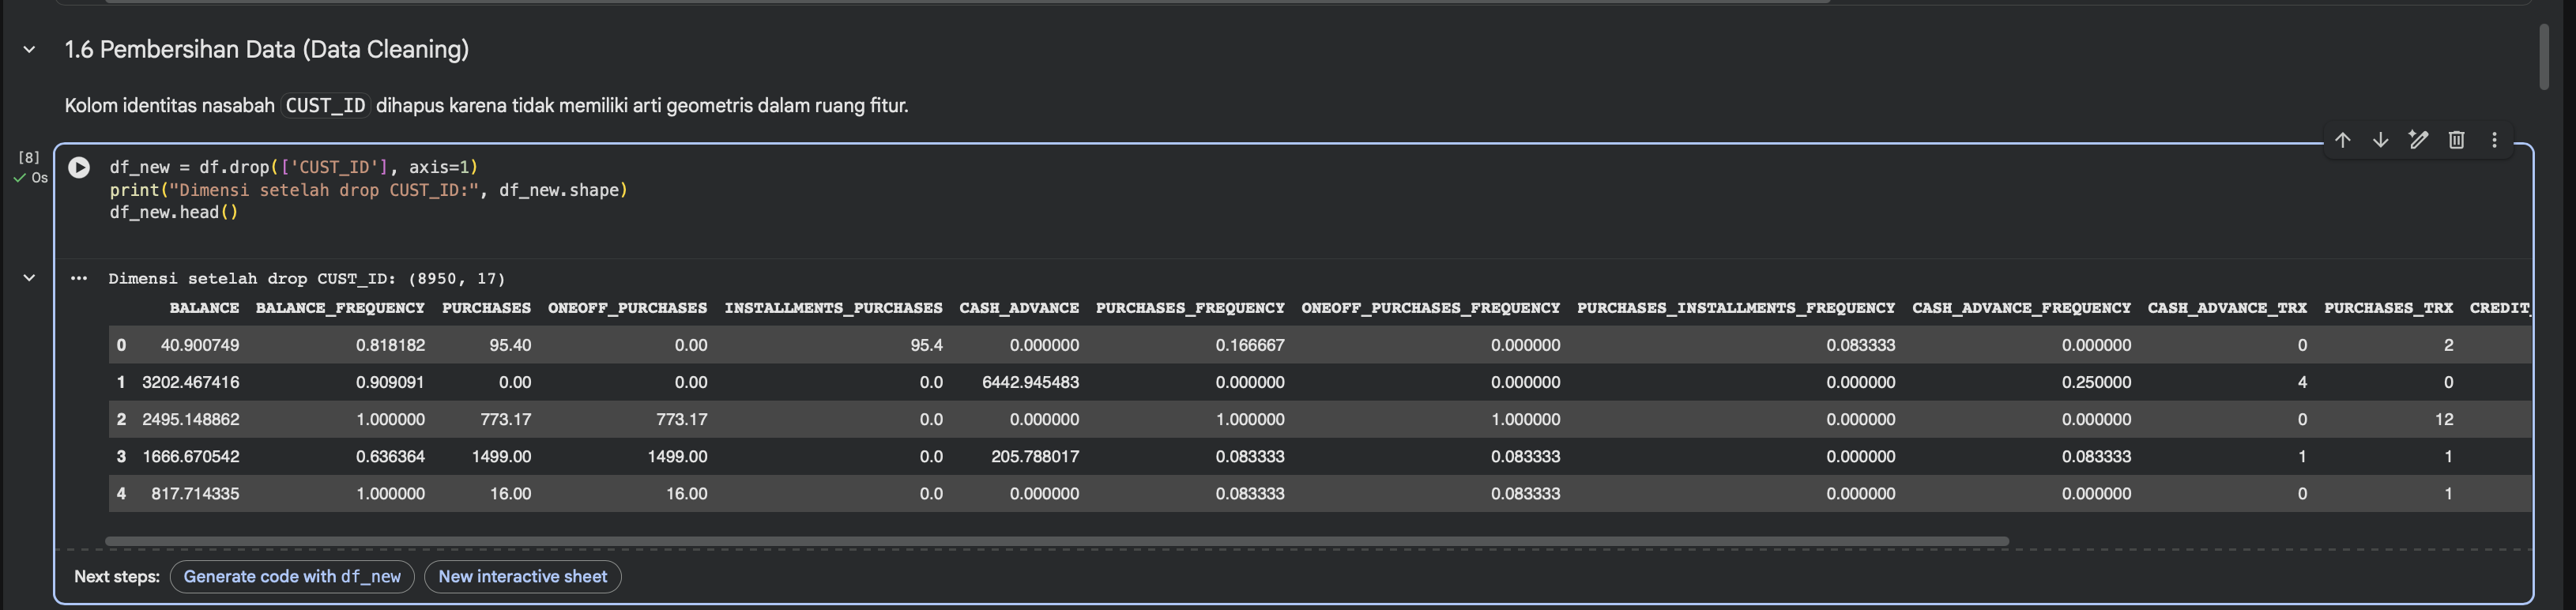
\includegraphics[width=0.9\textwidth]{images/ss-05-drop-custid.png}}
\caption{Tangkapan layar penghapusan kolom CUST\_ID.}
\label{fig:ss-drop-custid}
\end{figure}

Pemeriksaan nilai hilang mendeteksi 1 nilai kosong pada kolom \texttt{CREDIT\_LIMIT} dan 313 nilai kosong pada kolom \texttt{MINIMUM\_PAYMENTS}.

\begin{lstlisting}[style=pythonstyle,caption={Pemeriksaan jumlah nilai hilang pada setiap kolom.}]
df_new.isnull().sum()
\end{lstlisting}

\begin{figure}[H]
\centering
\customfbox{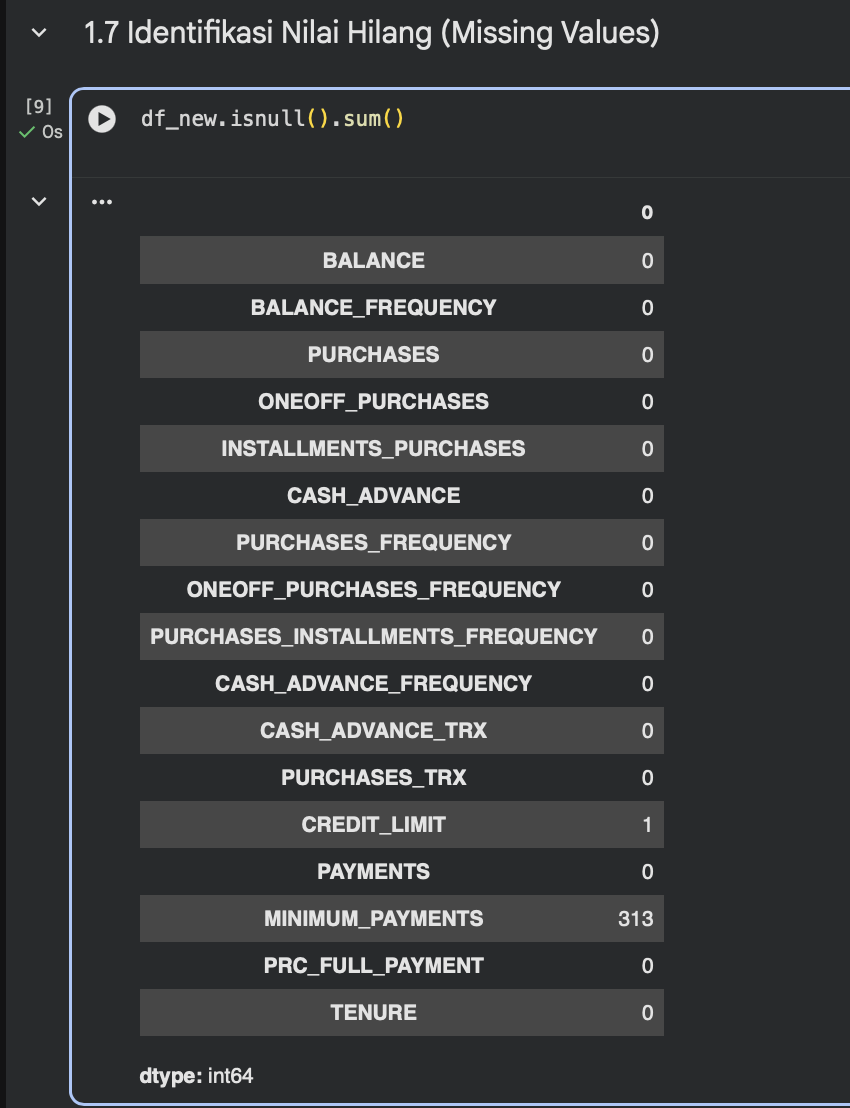
\includegraphics[width=0.45\textwidth]{images/ss-06-null-awal.png}}
\caption{Tangkapan layar pemeriksaan nilai hilang sebelum imputasi.}
\label{fig:ss-null-awal}
\end{figure}

Imputasi nilai hilang dilakukan memakai nilai median dari masing-masing fitur bersangkutan. Median dipilih agar pengisian data tidak terpengaruh oleh sebaran nilai ekstrem (outlier). Setelah imputasi dijalankan, pemeriksaan ulang mengonfirmasi bahwa seluruh kolom telah terisi penuh.

\begin{lstlisting}[style=pythonstyle,caption={Imputasi nilai hilang dengan median dan verifikasi hasil.}]
df_new['MINIMUM_PAYMENTS'].fillna(df_new['MINIMUM_PAYMENTS'].median(), inplace=True)
df_new['CREDIT_LIMIT'].fillna(df_new['CREDIT_LIMIT'].median(), inplace=True)
df_new.isnull().sum()
\end{lstlisting}

\begin{figure}[H]
\centering
\customfbox{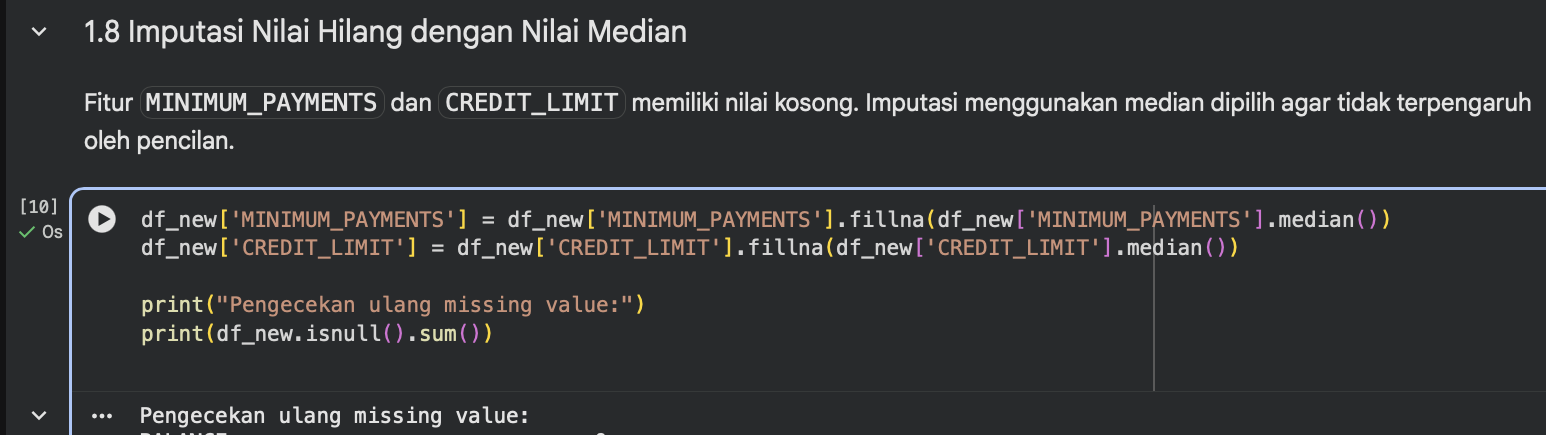
\includegraphics[width=0.85\textwidth]{images/ss-07-imputasi.png}}
\caption{Tangkapan layar kode imputasi median.}
\label{fig:ss-imputasi}
\end{figure}

\begin{figure}[H]
\centering
\customfbox{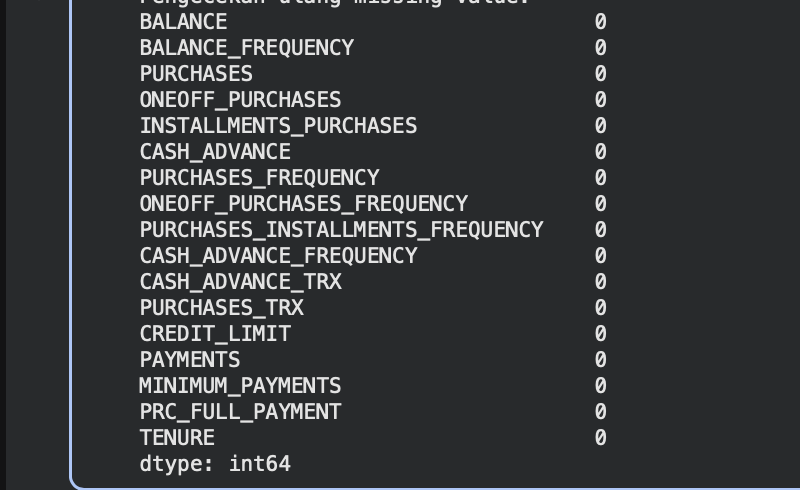
\includegraphics[width=0.55\textwidth]{images/ss-08-null-akhir.png}}
\caption{Tangkapan layar verifikasi data setelah imputasi selesai.}
\label{fig:ss-null-akhir}
\end{figure}

\subsection{Standarisasi Skala Fitur Data}
Rentang nilai antar-fitur sangat timpang. Misalnya kolom \texttt{BALANCE} mencapai ribuan dolar, sedangkan frekuensi transaksi berada pada skala 0 sampai 1. Seluruh 17 fitur numerik distandarisasi memakai \texttt{StandardScaler} agar memiliki rata-rata $\mu = 0$ dan simpangan baku $\sigma = 1$. Langkah ini mencegah fitur dengan satuan besar mendominasi perhitungan jarak Euclidean.

\begin{lstlisting}[style=pythonstyle,caption={Standarisasi fitur memakai StandardScaler.}]
X = df_new.astype(float).values
scaler = StandardScaler().fit(X)
X_new = scaler.transform(X)
X_new
\end{lstlisting}

\begin{figure}[H]
\centering
\customfbox{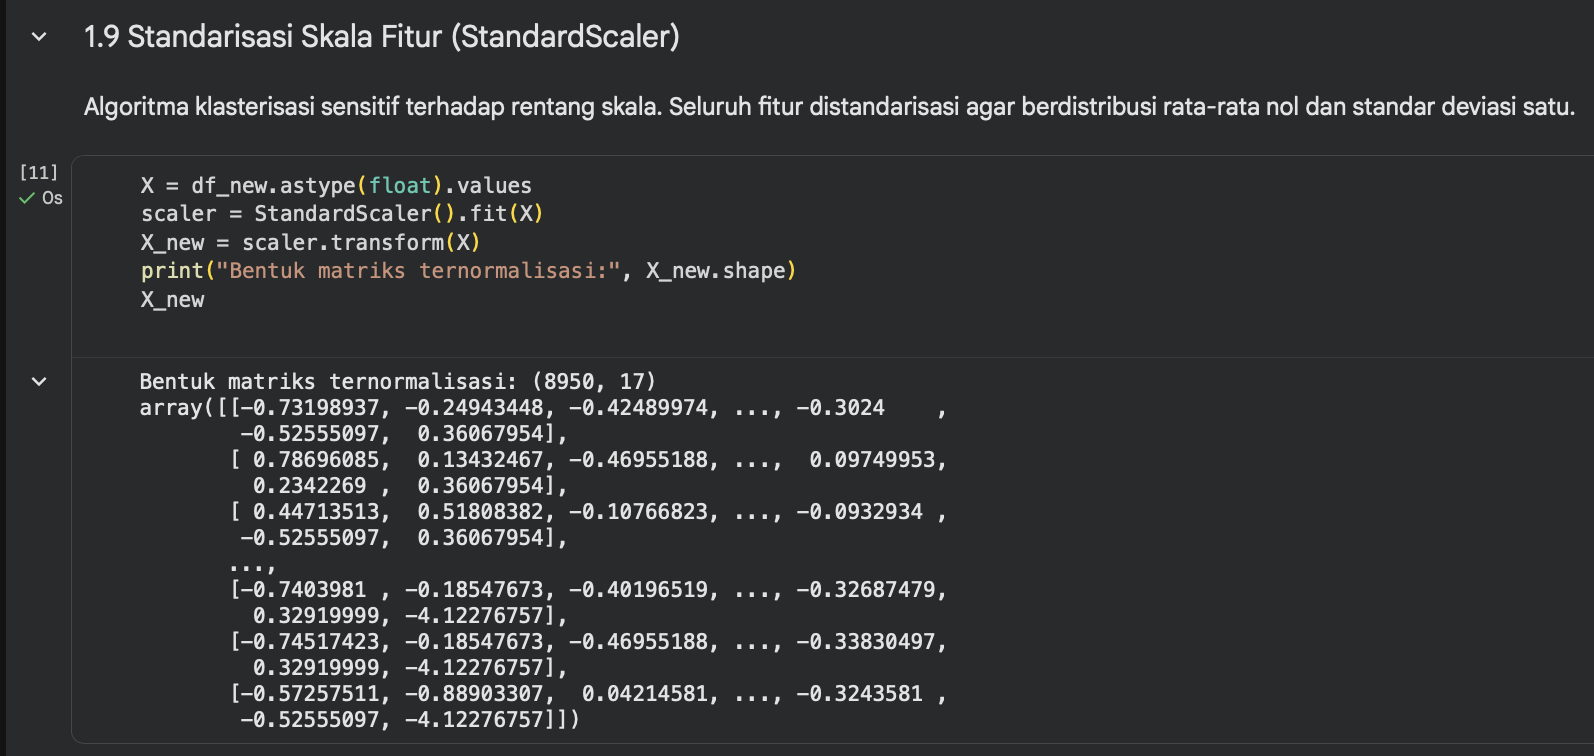
\includegraphics[width=0.85\textwidth]{images/ss-09-scaling.png}}
\caption{Tangkapan layar matriks fitur ternormalisasi StandardScaler.}
\label{fig:ss-scaling}
\end{figure}

\subsection{Penentuan Nilai K Optimal pada K-Means}
Saya menguji model K-Means untuk rentang nilai $K = 1$ sampai $10$ dengan mencatat nilai inertia (WCSS) pada setiap percobaan.

\begin{lstlisting}[style=pythonstyle,caption={Pengujian nilai inertia K-Means untuk K = 1 hingga 10.}]
inertia_list = []
for num_clusters in range(1, 11):
    kmeans_model = KMeans(n_clusters=num_clusters, random_state=42)
    kmeans_model.fit(X_new)
    inertia_list.append(kmeans_model.inertia_)
    print("For n_clusters = {}, inertia value is {}".format(
        num_clusters, kmeans_model.inertia_))
\end{lstlisting}

\begin{figure}[H]
\centering
\customfbox{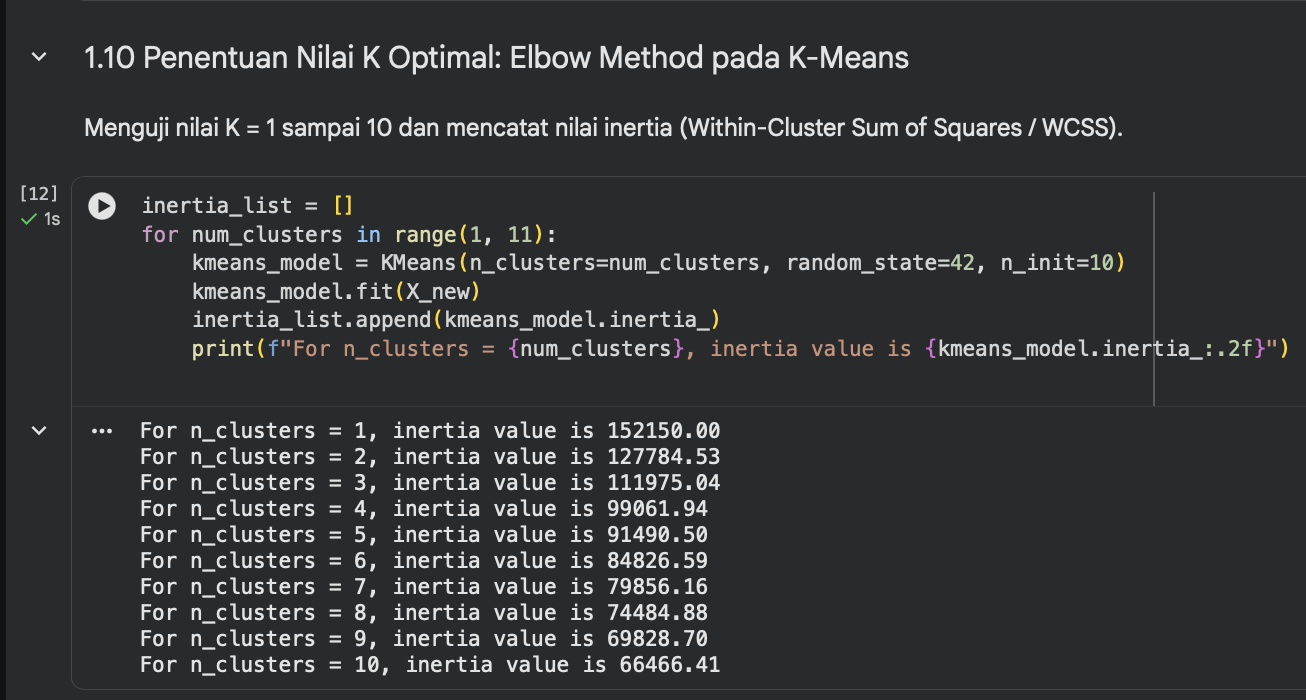
\includegraphics[width=0.85\textwidth]{images/ss-10-inertia-kmeans.png}}
\caption{Tangkapan layar pencatatan nilai inertia K-Means.}
\label{fig:ss-inertia-kmeans}
\end{figure}

Hasil perhitungan inertia dirangkum pada Tabel~\ref{tab:evaluasi-k-kmeans}.

\begin{table}[H]
\centering
\small
\begin{tabular}{ccc}
\toprule
\textbf{Jumlah Klaster ($K$)} & \textbf{Inertia (WCSS)} & \textbf{Silhouette Score} \\
\midrule
1 & 152.150{,}00 & - \\
2 & 127.784{,}71 & 0{,}2095 \\
3 & 111.975{,}04 & 0{,}2504 \\
4 & 99.061{,}94 & 0{,}1977 \\
5 & 91.491{,}11 & 0{,}1933 \\
6 & 84.825{,}07 & 0{,}2027 \\
7 & 79.551{,}38 & 0{,}2150 \\
8 & 74.467{,}92 & 0{,}2184 \\
9 & 69.832{,}80 & 0{,}2150 \\
10 & 66.459{,}92 & 0{,}2193 \\
\bottomrule
\end{tabular}
\caption{Evaluasi nilai Inertia dan Silhouette Score pada K-Means.}
\label{tab:evaluasi-k-kmeans}
\end{table}

Saya memplot kurva inertia untuk mengamati titik siku. Pendeteksian siku secara objektif dilakukan menggunakan modul \texttt{KneeLocator} dari pustaka \texttt{kneed}.

\begin{lstlisting}[style=pythonstyle,caption={Pembuatan plot kurva inertia dan deteksi KneeLocator.}]
plt.plot(range(1, 11), inertia_list, marker='o', linewidth=2, markersize=8)
plt.xlabel("Number of Clusters", size=13)
plt.ylabel("Inertia Value", size=13)
plt.title("Inertia values vary depending on clusters utilized.")
plt.show()

from kneed import KneeLocator
kneedle = KneeLocator(
    range(1, 11), inertia_list,
    S=1.0, curve='convex', direction='decreasing'
)
print("Optimal Knee Point:", round(kneedle.knee, 3))
print("Optimal Elbow Point:", round(kneedle.elbow, 3))

plt.style.use('ggplot')
kneedle.plot_knee()
plt.show()
\end{lstlisting}

\begin{figure}[H]
\centering
\customfbox{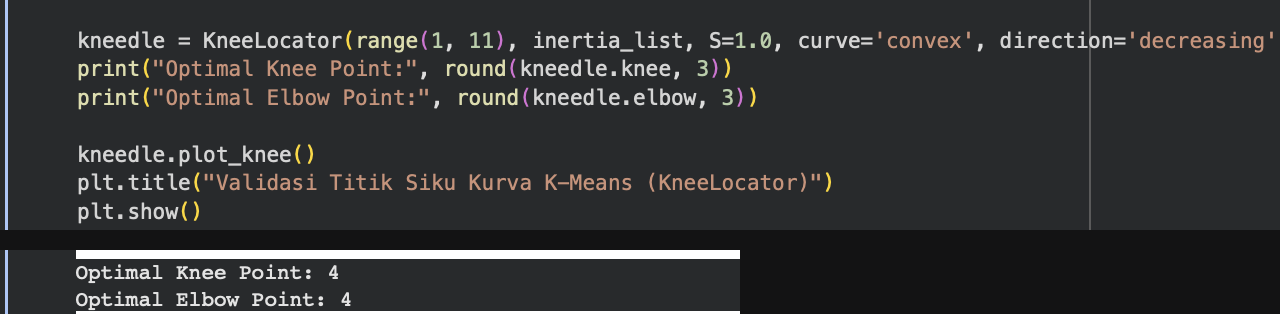
\includegraphics[width=0.75\textwidth]{images/ss-12-kneed-kmeans.png}}
\caption{Tangkapan layar luaran deteksi titik siku optimal KneeLocator K = 4.}
\label{fig:ss-kneed-kmeans}
\end{figure}

\begin{figure}[H]
\centering
\begin{minipage}[b]{0.48\textwidth}
    \centering
    \customfbox{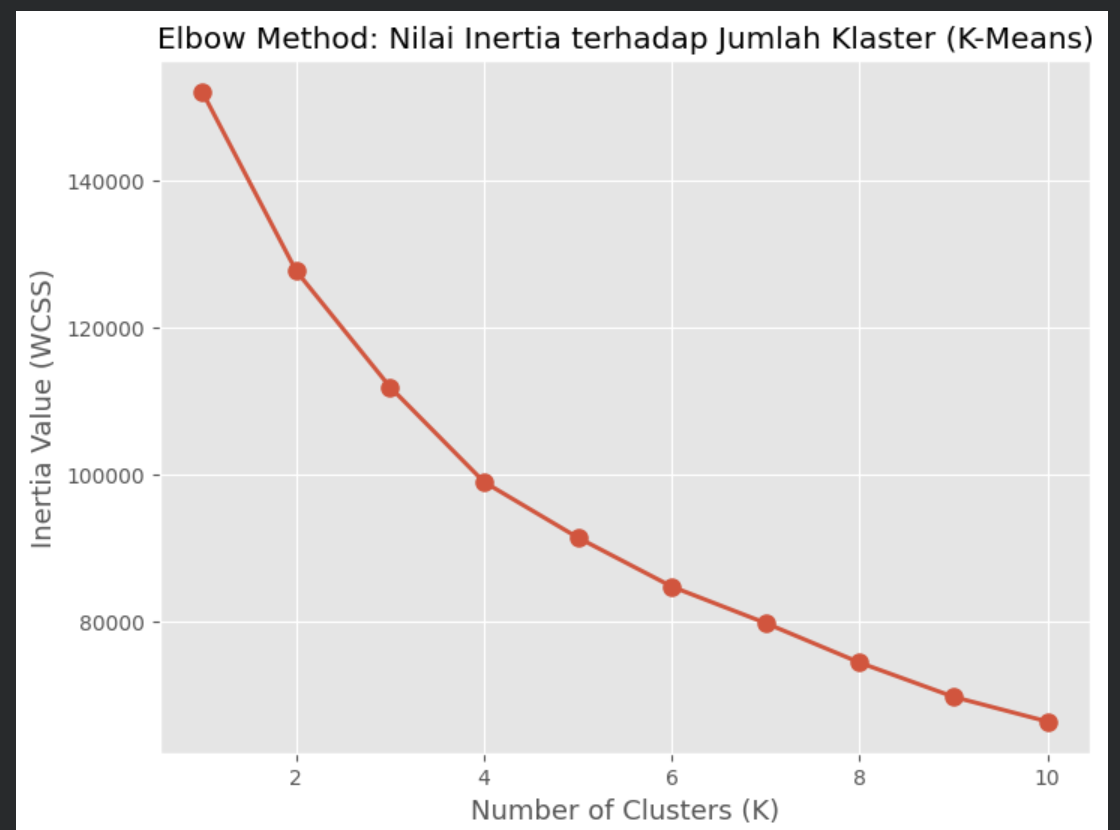
\includegraphics[width=\dimexpr\linewidth-1pt\relax]{images/ss-11-plot-elbow-kmeans.png}}
    \caption{Kurva Elbow Method K-Means.}
    \label{fig:ss-plot-elbow-kmeans}
\end{minipage}
\hfill
\begin{minipage}[b]{0.48\textwidth}
    \centering
    \customfbox{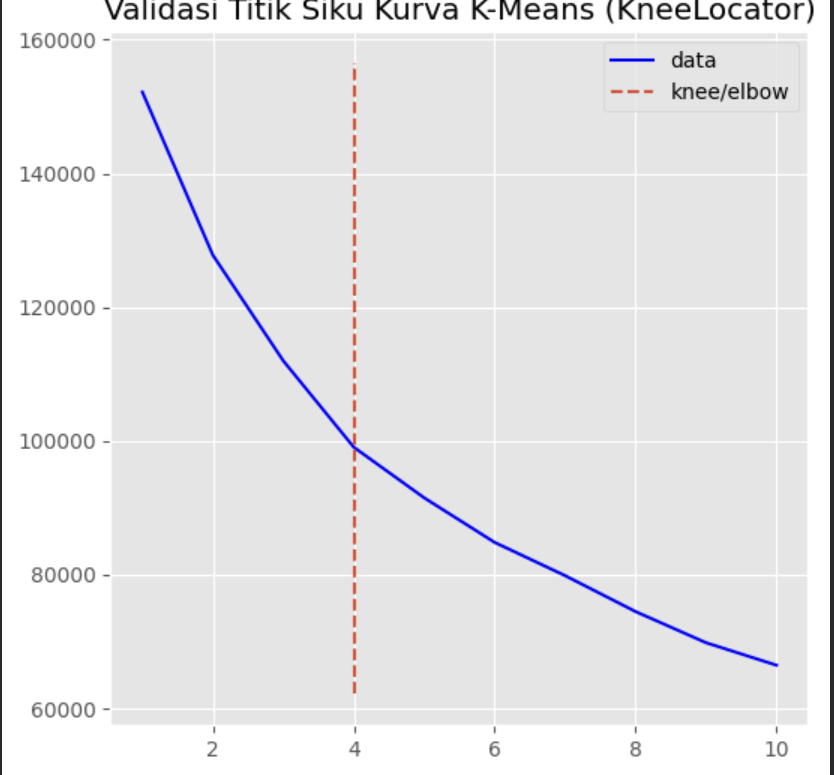
\includegraphics[width=\dimexpr\linewidth-1pt\relax]{images/ss-13-kneedle-plot-kmeans.png}}
    \caption{Plot konfirmasi titik siku K = 4.}
    \label{fig:ss-kneedle-plot-kmeans}
\end{minipage}
\end{figure}

KneeLocator mengonfirmasi titik siku optimal pada $K = 4$. Setelah titik $K = 4$, laju penurunan inertia melandai.

\subsection{Penentuan Nilai K Optimal pada K-Medoids}
Eksperimen serupa dilakukan memakai \texttt{KMedoids} dari \texttt{sklearn\_extra.cluster} untuk nilai $K = 1$ sampai $10$.

\begin{lstlisting}[style=pythonstyle,caption={Evaluasi nilai inertia K-Medoids.}]
from sklearn_extra.cluster import KMedoids

inertia_list_kmed = []
for num_clusters in range(1, 11):
    kmedoids_model = KMedoids(n_clusters=num_clusters, random_state=42)
    kmedoids_model.fit(X_new)
    inertia_list_kmed.append(kmedoids_model.inertia_)
    print(f"The inertia of {num_clusters} clusters : {kmedoids_model.inertia_}")
\end{lstlisting}

\begin{figure}[H]
\centering
\customfbox{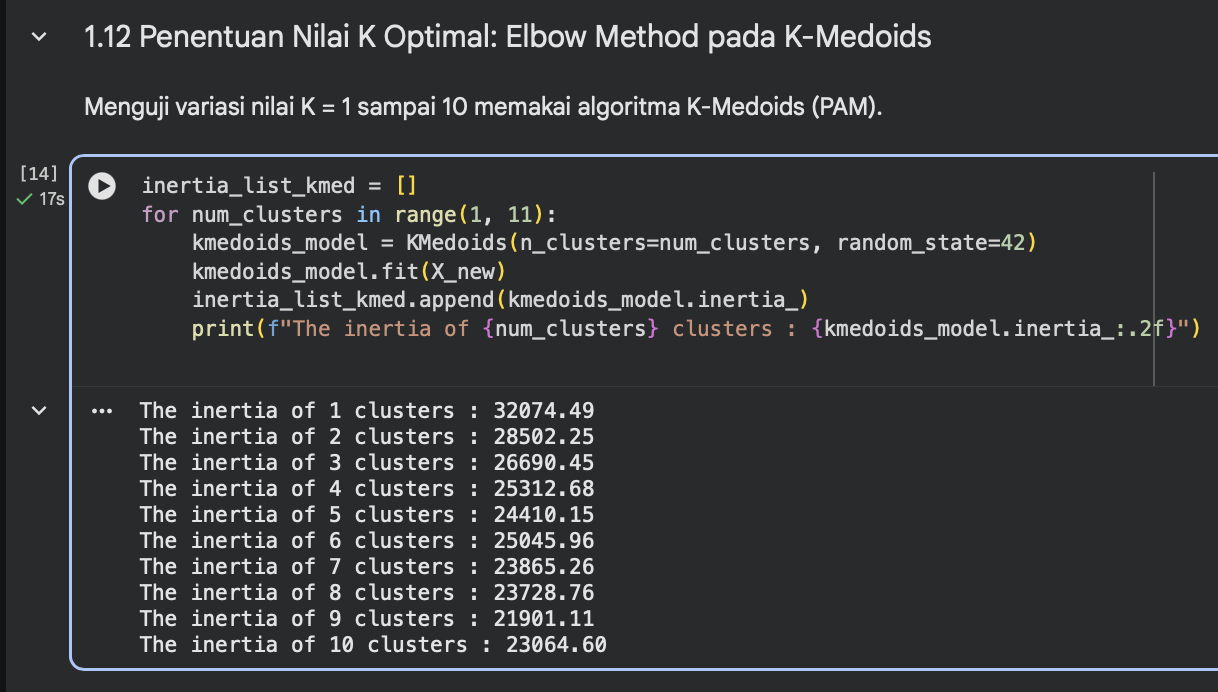
\includegraphics[width=0.75\textwidth]{images/ss-14-inertia-kmedoids.png}}
\caption{Tangkapan layar perhitungan inertia K-Medoids.}
\label{fig:ss-inertia-kmedoids}
\end{figure}

Nilai inertia K-Medoids pada $K=1$ bernilai 32.074{,}49, lalu turun ke 28.502{,}25 ($K=2$), 26.690{,}45 ($K=3$), 25.312{,}68 ($K=4$), dan 24.410{,}15 ($K=5$). Penerapan \texttt{KneeLocator} pada K-Medoids juga menghasilkan titik siku pada $K = 4$.

\begin{lstlisting}[style=pythonstyle,caption={Visualisasi kurva elbow dan deteksi titik siku K-Medoids.}]
plt.plot(range(1, 11), inertia_list_kmed, marker='o', linewidth=2, markersize=8)
plt.xlabel("Number of Clusters", size=13)
plt.ylabel("Inertia Value", size=13)
plt.title("Inertia values vary depending on clusters utilized.")
plt.show()

kneedle_med = KneeLocator(
    range(1, 11), inertia_list_kmed,
    S=1.0, curve='convex', direction='decreasing'
)
print("Knee point K-Medoids:", kneedle_med.knee)
kneedle_med.plot_knee()
plt.show()
\end{lstlisting}

\begin{figure}[H]
\centering
\begin{minipage}[b]{0.48\textwidth}
    \centering
    \customfbox{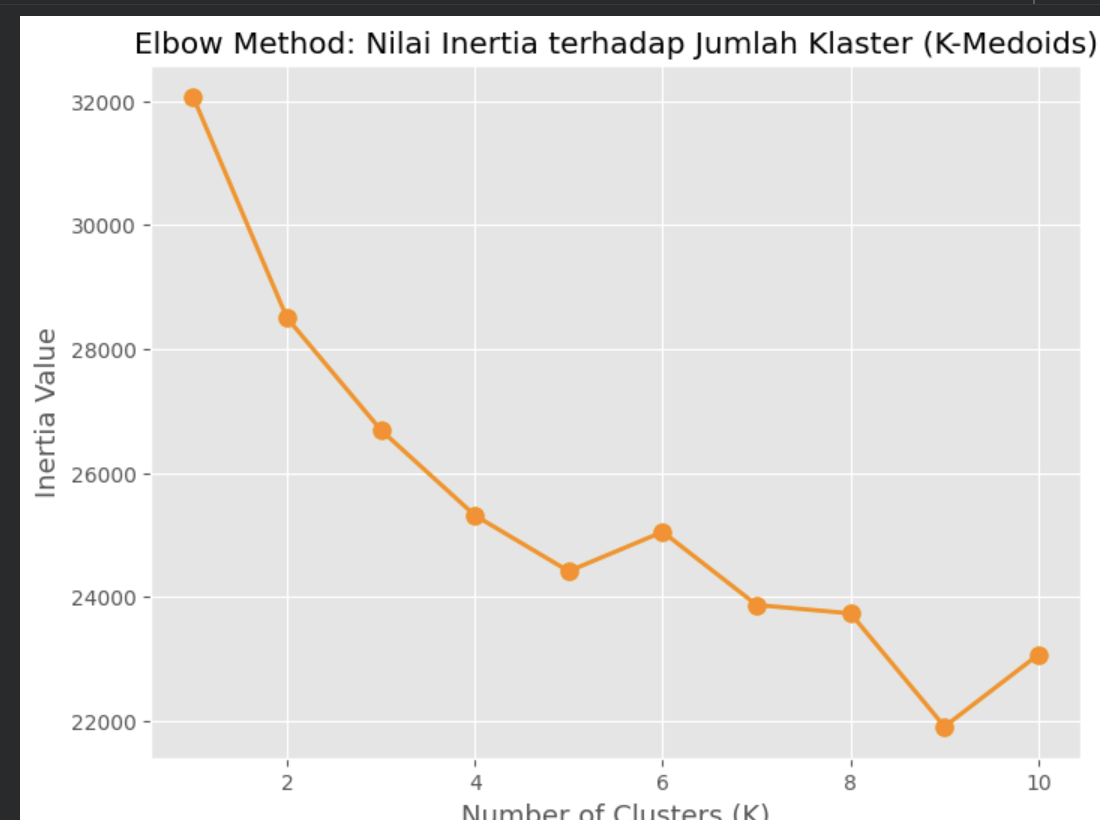
\includegraphics[width=\dimexpr\linewidth-1pt\relax]{images/ss-15-plot-elbow-kmedoids.png}}
    \caption{Kurva Elbow Method K-Medoids.}
    \label{fig:ss-plot-elbow-kmedoids}
\end{minipage}
\hfill
\begin{minipage}[b]{0.48\textwidth}
    \centering
    \customfbox{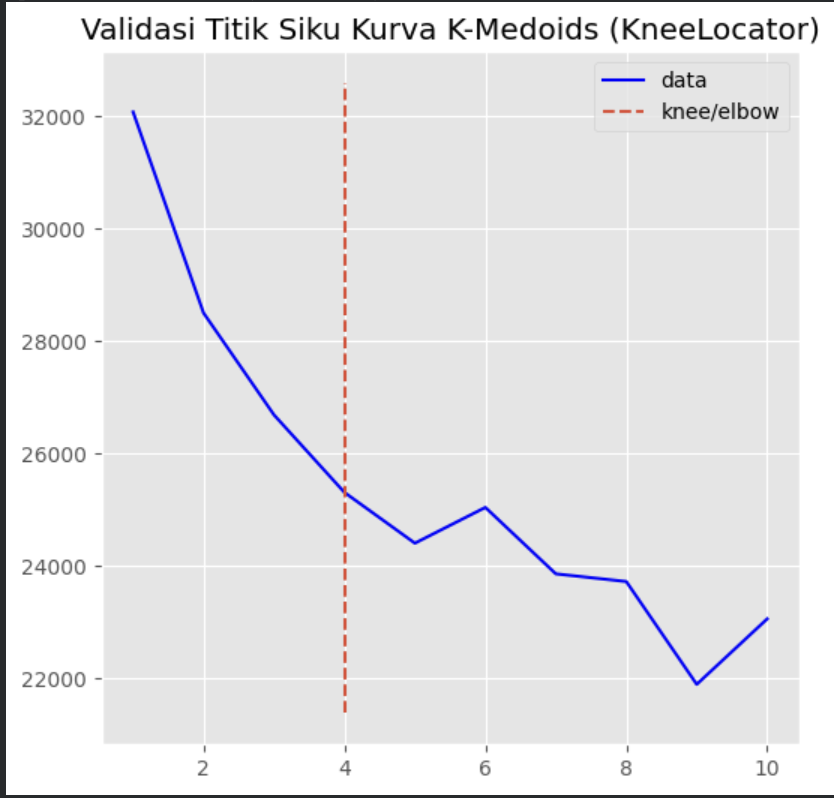
\includegraphics[width=\dimexpr\linewidth-1pt\relax]{images/ss-16-kneed-kmedoids.png}}
    \caption{Validasi titik siku K-Medoids K = 4.}
    \label{fig:ss-kneed-kmedoids}
\end{minipage}
\end{figure}

\subsection{Evaluasi Silhouette Score pada K-Means dan K-Medoids}
Evaluasi skor siluet dilakukan pada rentang $K = 2$ sampai $10$.

\begin{lstlisting}[style=pythonstyle,caption={Perhitungan dan visualisasi Silhouette Score K-Means.}]
sh_list = []
for num_clusters in range(2, 11):
    kmeans = KMeans(n_clusters=num_clusters, random_state=42)
    cluster_labels = kmeans.fit_predict(X_new)
    score = silhouette_score(X_new, cluster_labels)
    sh_list.append(score)
    print("For n_clusters = {}, silhouette score is {}".format(
        num_clusters, score))

plt.plot(range(2, 11), sh_list, marker='o', linewidth=2, markersize=8)
plt.xlabel("Number of Clusters", size=13)
plt.ylabel("silhouette score", size=13)
plt.title("Silhouette score vary depending on clusters utilized.")
plt.show()
\end{lstlisting}

\begin{figure}[H]
\centering
\begin{minipage}[b]{0.48\textwidth}
    \centering
    \customfbox{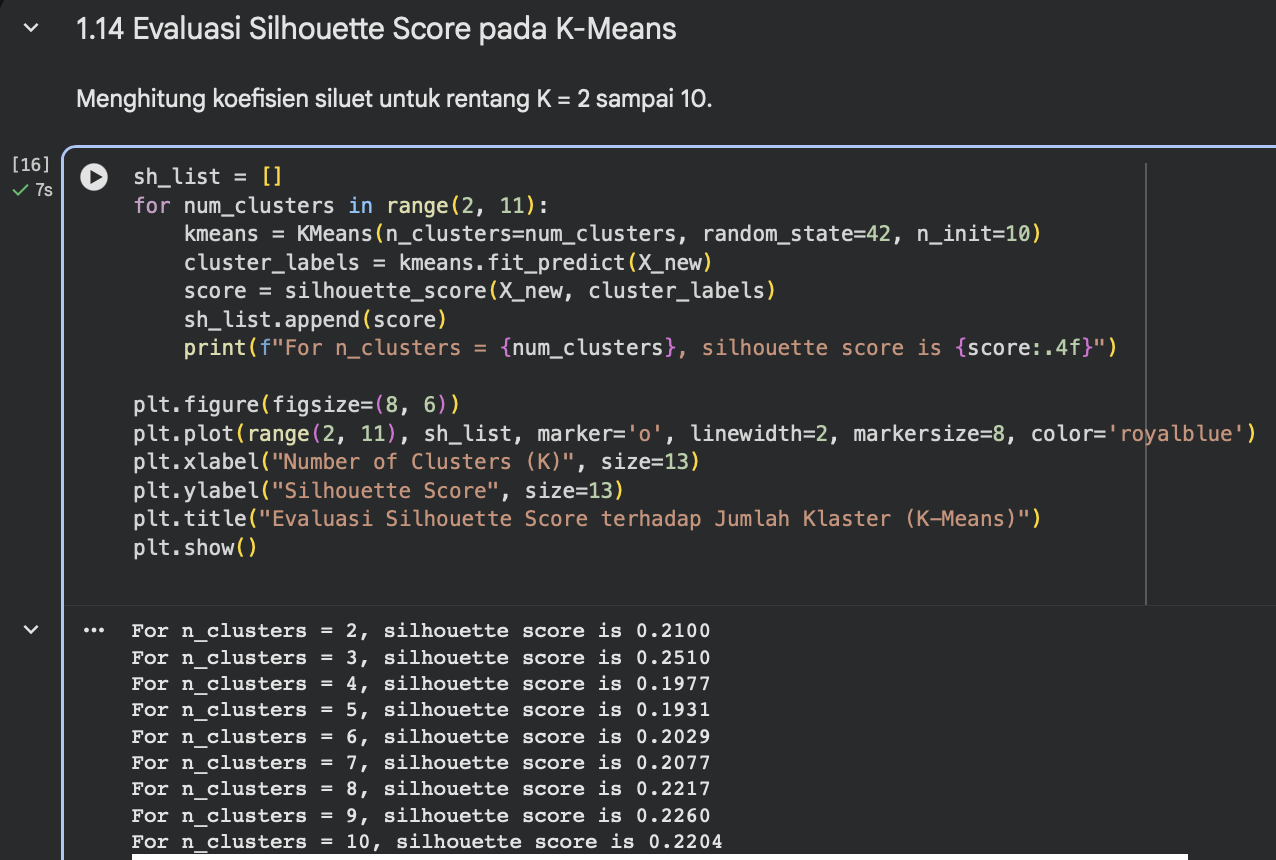
\includegraphics[width=\dimexpr\linewidth-1pt\relax]{images/ss-17-sil-score-kmeans.png}}
    \caption{Perhitungan Silhouette K-Means.}
    \label{fig:ss-sil-score-kmeans}
\end{minipage}
\hfill
\begin{minipage}[b]{0.48\textwidth}
    \centering
    \customfbox{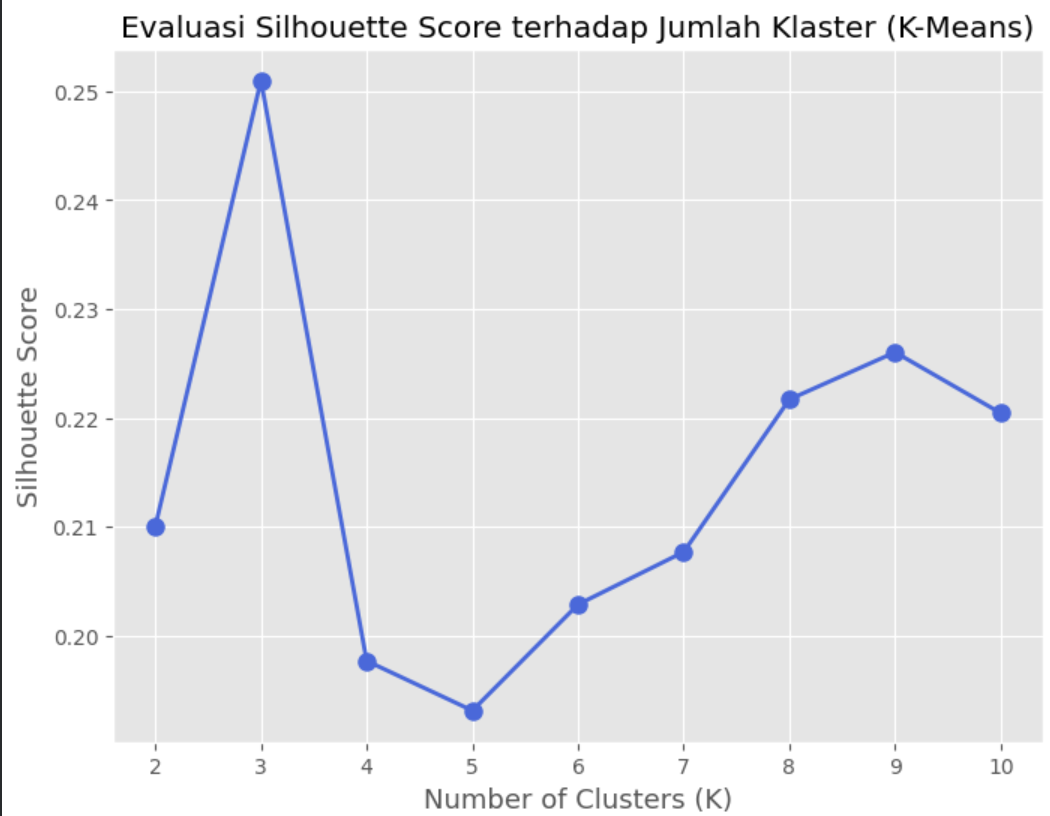
\includegraphics[width=\dimexpr\linewidth-1pt\relax]{images/ss-18-plot-sil-kmeans.png}}
    \caption{Kurva Silhouette Score K-Means.}
    \label{fig:ss-plot-sil-kmeans}
\end{minipage}
\end{figure}

Pada K-Means, nilai siluet tertinggi berada pada $K = 3$ dengan skor 0{,}2504, disusul $K = 10$ (0{,}2193), $K = 8$ (0{,}2184), dan $K = 4$ (0{,}1977). Meskipun $K = 3$ menghasilkan skor siluet tertinggi, $K = 4$ dipilih karena titik siku Elbow Method secara konsisten berada pada $K = 4$, dan empat kelompok memberikan pemisahan segmen bisnis nasabah yang lebih informatif dibandingkan tiga kelompok.

Pada K-Medoids, skor siluet pada $K = 2$ adalah 0{,}1945, $K = 3$ adalah 0{,}1602, $K = 4$ adalah 0{,}1374, dan terus menurun hingga 0{,}0347 pada $K = 10$.

\begin{lstlisting}[style=pythonstyle,caption={Perhitungan Silhouette Score K-Medoids.}]
sh_list_kmed = []
for num_clusters in range(2, 11):
    kmedoids = KMedoids(n_clusters=num_clusters, random_state=42)
    cluster_labels = kmedoids.fit_predict(X_new)
    score = silhouette_score(X_new, cluster_labels)
    sh_list_kmed.append(score)
    print("For n_clusters = {}, silhouette score is {}".format(
        num_clusters, score))

plt.plot(range(2, 11), sh_list_kmed, marker='o', linewidth=2, markersize=8)
plt.xlabel("Number of Clusters", size=13)
plt.ylabel("silhouette score", size=13)
plt.title("Silhouette score vary depending on clusters utilized.")
plt.show()
\end{lstlisting}

\begin{figure}[H]
\centering
\begin{minipage}[b]{0.48\textwidth}
    \centering
    \customfbox{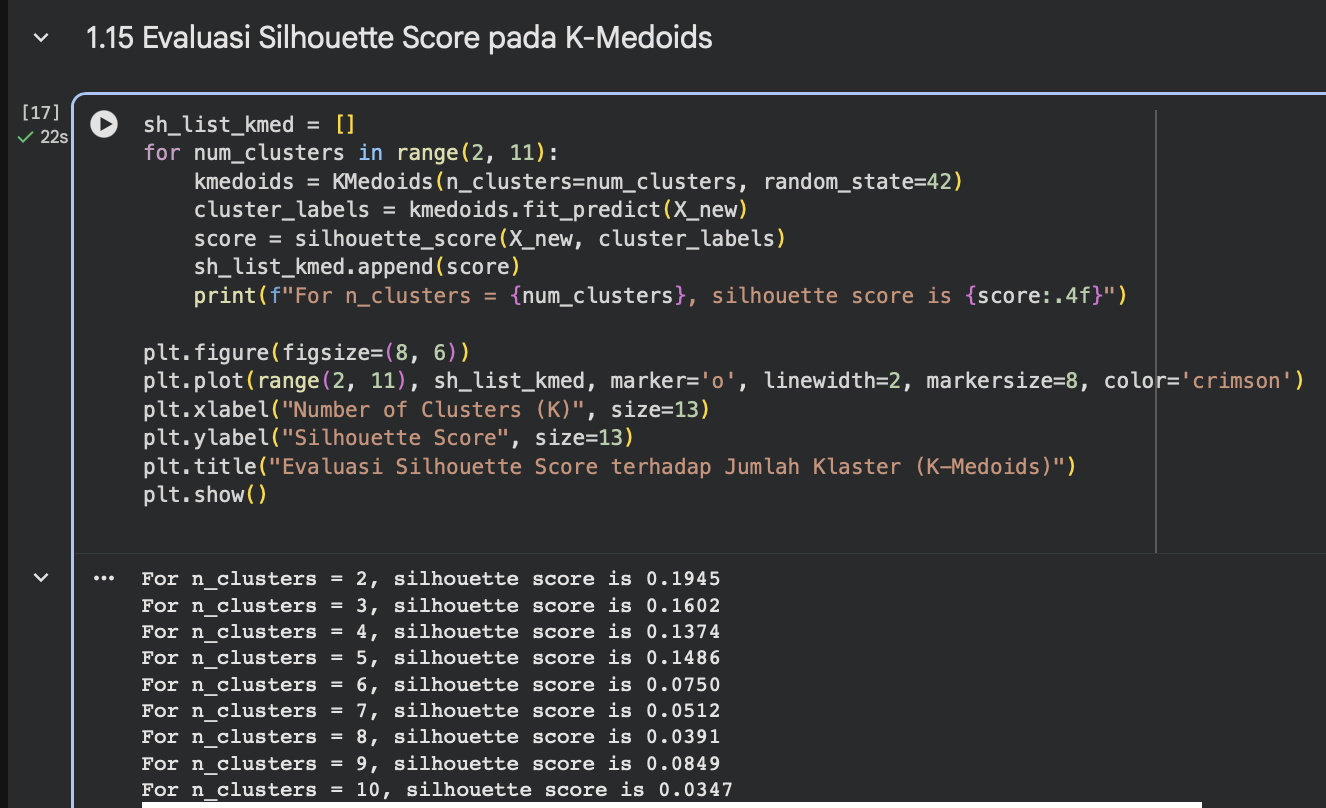
\includegraphics[width=\dimexpr\linewidth-1pt\relax]{images/ss-19-sil-score-kmedoids.png}}
    \caption{Perhitungan Silhouette K-Medoids.}
    \label{fig:ss-sil-score-kmedoids}
\end{minipage}
\hfill
\begin{minipage}[b]{0.48\textwidth}
    \centering
    \customfbox{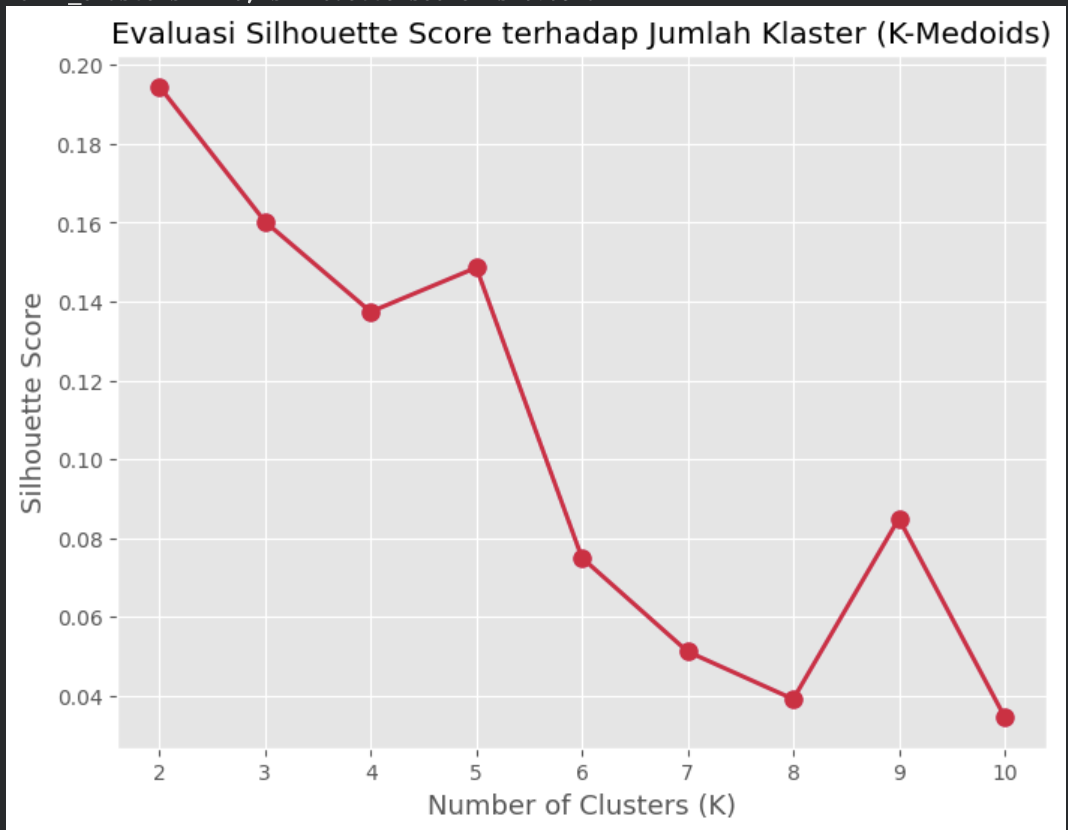
\includegraphics[width=\dimexpr\linewidth-1pt\relax]{images/ss-20-plot-sil-kmedoids.png}}
    \caption{Kurva Silhouette K-Medoids.}
    \label{fig:ss-plot-sil-kmedoids}
\end{minipage}
\end{figure}

\subsection{Pelatihan Model K-Means (K = 4) dan Visualisasi}
Model K-Means dilatih secara definitif memakai $K = 4$ dengan parameter \texttt{random\_state=42}. Label hasil pengelompokan disimpan pada kolom \texttt{cluster\_labels}.

\begin{lstlisting}[style=pythonstyle,caption={Pelatihan K-Means K = 4 dan pemeriksaan centroid.}]
k_means = KMeans(n_clusters=4, random_state=42)
k_means.fit(X_new)
labels = k_means.labels_
df_new['cluster_labels'] = labels

centroids = k_means.cluster_centers_
centroids
\end{lstlisting}

\begin{figure}[H]
\centering
\customfbox{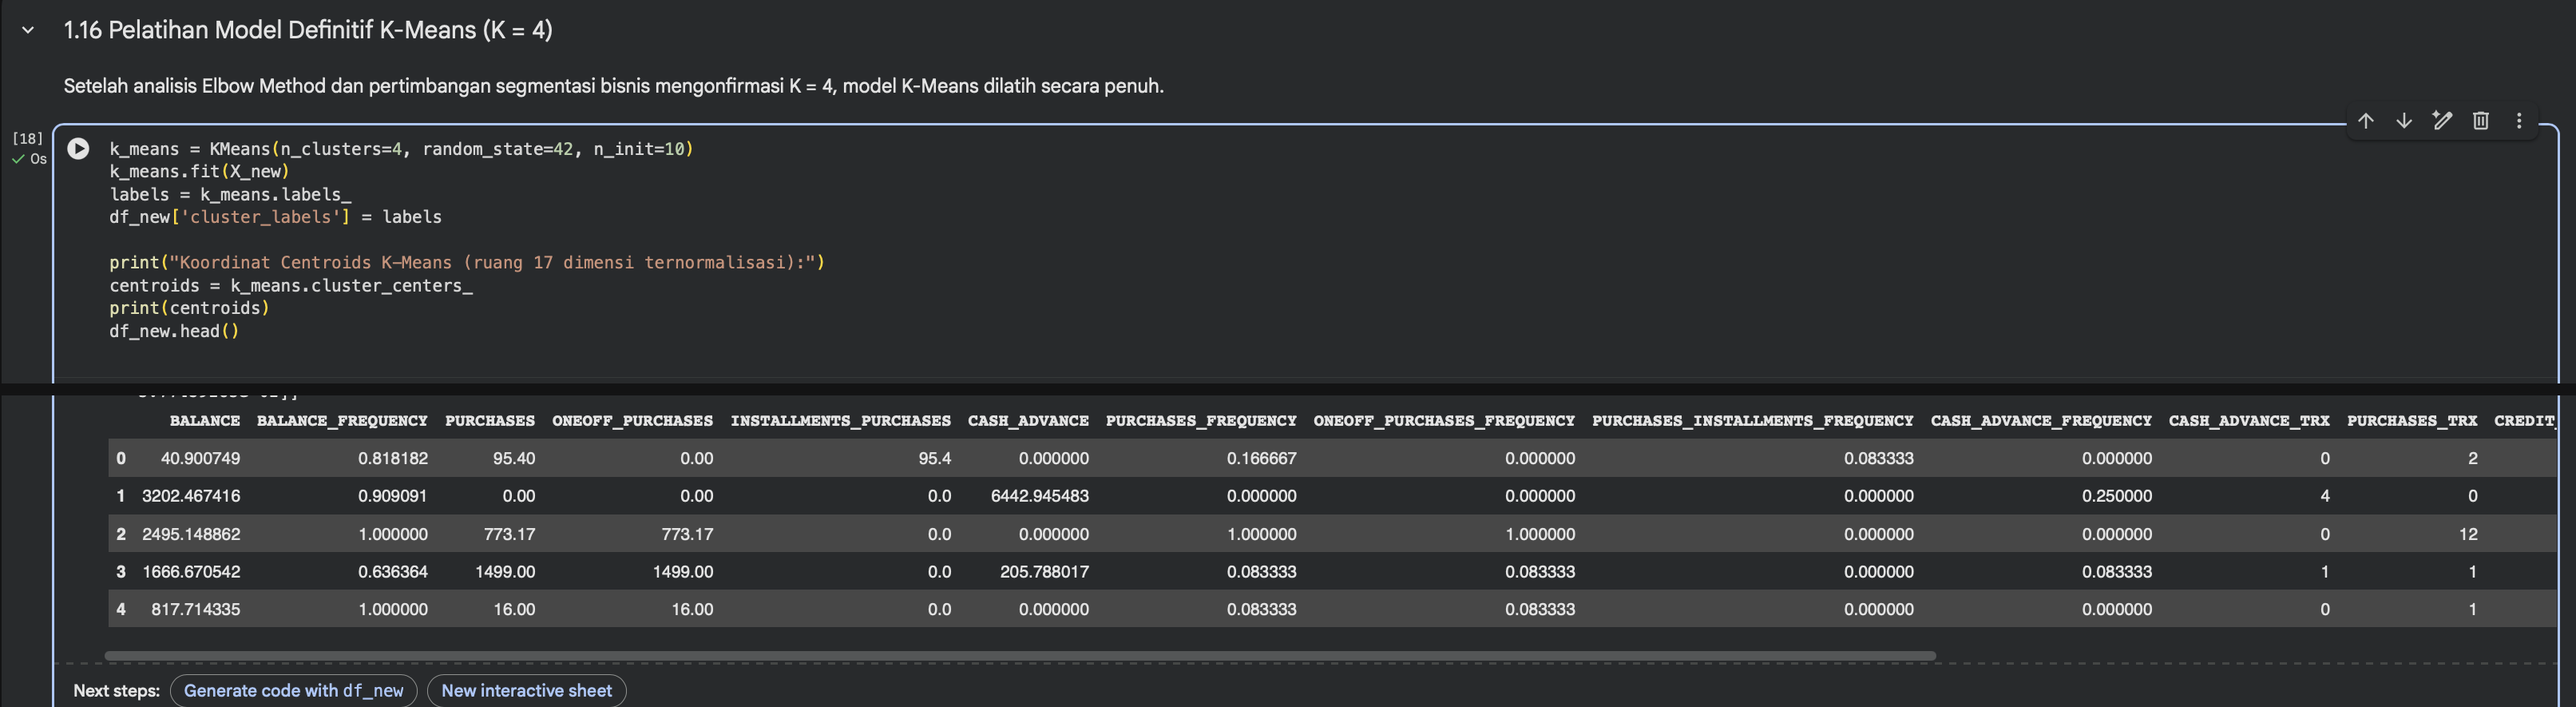
\includegraphics[width=0.85\textwidth]{images/ss-21-train-kmeans.png}}
\caption{Tangkapan layar penambahan label klaster K-Means pada dataframe.}
\label{fig:ss-train-kmeans}
\end{figure}

\begin{figure}[H]
\centering
\customfbox{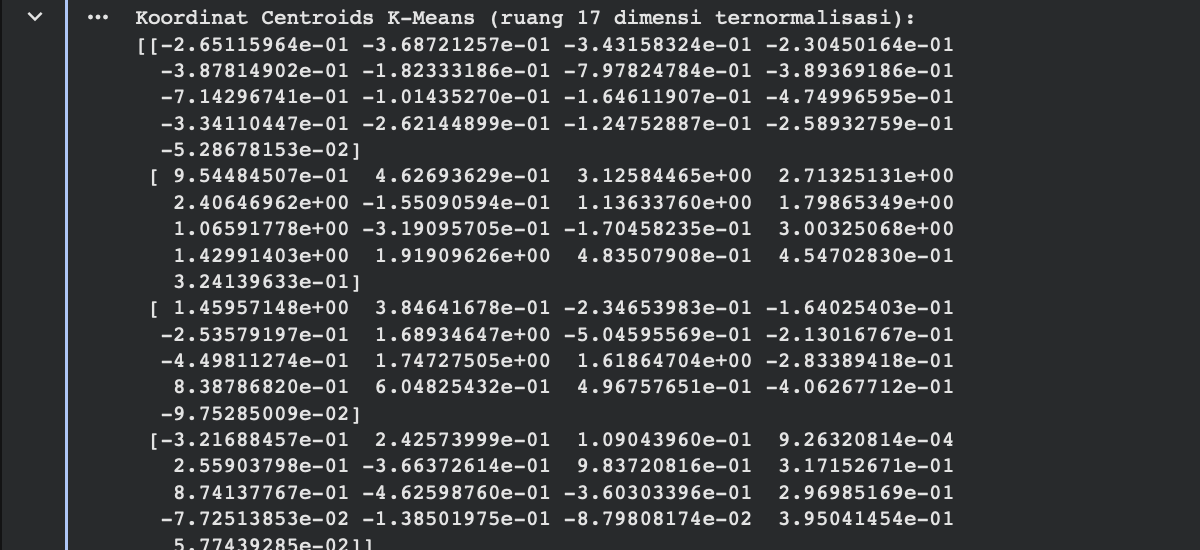
\includegraphics[width=0.75\textwidth]{images/ss-22-centroids-kmeans.png}}
\caption{Tangkapan layar koordinat centroid K-Means dalam ruang 17 dimensi.}
\label{fig:ss-centroids-kmeans}
\end{figure}

Sebaran klaster divisualisasikan dalam bentuk scatter plot 2 dimensi antara fitur \texttt{PURCHASES} dan \texttt{PAYMENTS} memakai Matplotlib dan Seaborn.

\begin{lstlisting}[style=pythonstyle,caption={Visualisasi 2 dimensi K-Means dengan Matplotlib dan Seaborn.}]
x1 = df_new['PURCHASES']
x2 = df_new['PAYMENTS']

plt.figure(figsize=(8, 6))
u_labels = np.unique(labels)
for i in u_labels:
    plt.scatter(x1[df_new['cluster_labels'] == i],
                x2[df_new['cluster_labels'] == i], label=i)
plt.xlabel(x1.name, fontsize=14)
plt.ylabel(x2.name, fontsize=14)
plt.title('K-means clustering', fontsize=16)
plt.legend()
plt.show()

plt.figure(figsize=(8, 6))
sns.scatterplot(
    x='PURCHASES', y='PAYMENTS',
    hue='cluster_labels', data=df_new, palette='Paired'
)
plt.legend(loc='lower right')
plt.title('K-Means Cluster Scatter Plot (Seaborn)')
plt.show()
\end{lstlisting}

\begin{figure}[H]
\centering
\begin{minipage}[b]{0.48\textwidth}
    \centering
    \customfbox{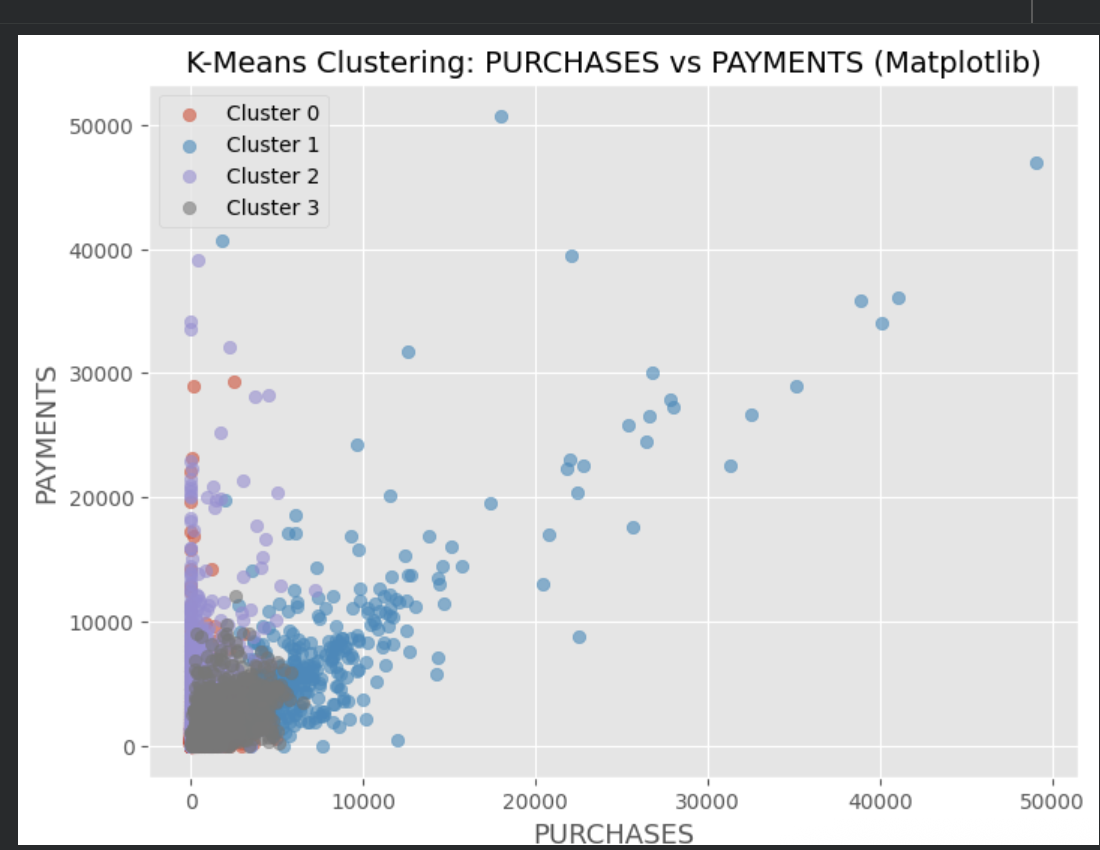
\includegraphics[width=\dimexpr\linewidth-1pt\relax]{images/ss-23-scatter-matplotlib-kmeans.png}}
    \caption{Visualisasi 2D K-Means (Matplotlib).}
    \label{fig:ss-scatter-matplotlib-kmeans}
\end{minipage}
\hfill
\begin{minipage}[b]{0.48\textwidth}
    \centering
    \customfbox{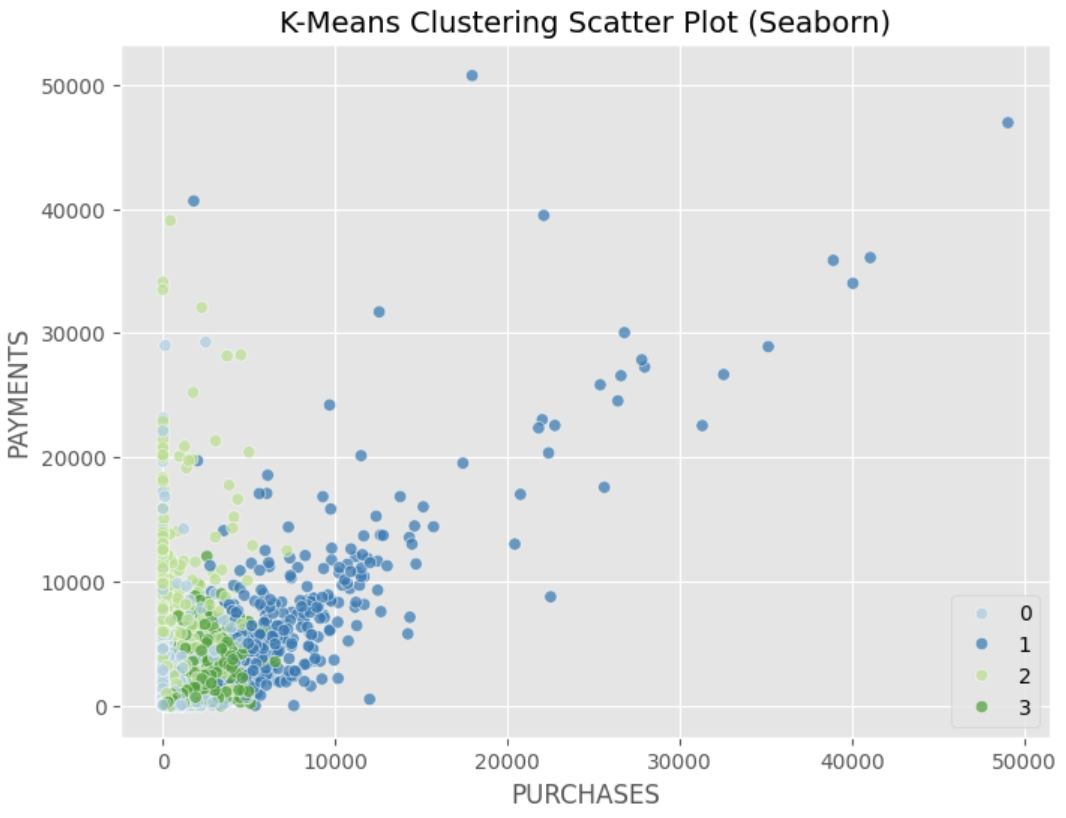
\includegraphics[width=\dimexpr\linewidth-1pt\relax]{images/ss-24-scatter-seaborn-kmeans.png}}
    \caption{Visualisasi 2D K-Means (Seaborn).}
    \label{fig:ss-scatter-seaborn-kmeans}
\end{minipage}
\end{figure}

Visualisasi interaktif 3 dimensi dibangun memakai Plotly Express dengan melibatkan tiga variabel finansial utama: \texttt{PURCHASES}, \texttt{PAYMENTS}, dan \texttt{BALANCE}.

\begin{lstlisting}[style=pythonstyle,caption={Visualisasi 3 dimensi K-Means memakai Plotly Express.}]
fig = px.scatter_3d(
    df_new, x='PURCHASES', y='PAYMENTS',
    z='BALANCE', color='cluster_labels'
)
fig.show()
\end{lstlisting}

\begin{figure}[H]
\centering
\customfbox{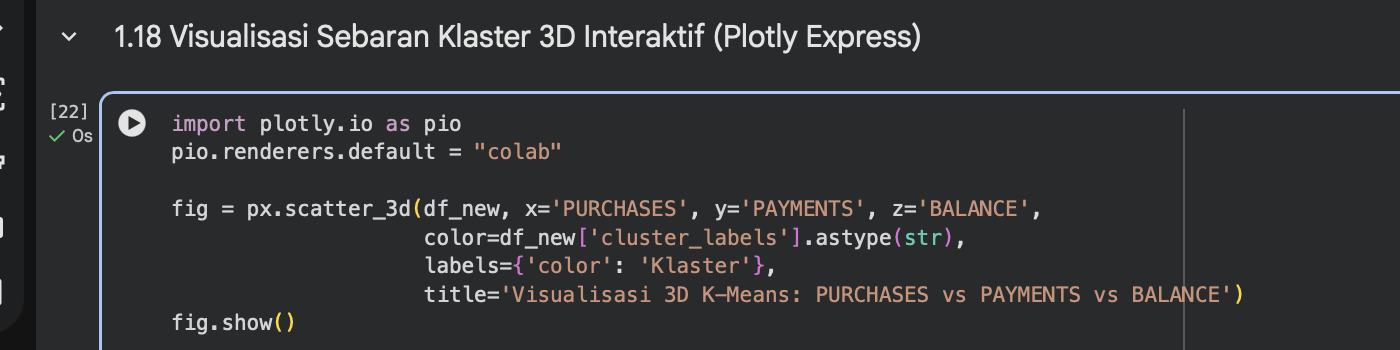
\includegraphics[width=0.8\textwidth]{images/ss-25-scatter-3d-kmeans.png}}
\caption{Tangkapan layar kode pembangkitan plot 3 dimensi Plotly Express.}
\label{fig:ss-scatter-3d-kmeans}
\end{figure}

\subsection{Pelatihan Model K-Medoids (K = 4) dan Visualisasi}
Model K-Medoids dilatih dengan parameter $K = 4$ dan \texttt{random\_state=42}. Label hasil pengelompokan disimpan pada kolom \texttt{cluster\_labels\_kmed}.

\begin{lstlisting}[style=pythonstyle,caption={Pelatihan K-Medoids K = 4 dan visualisasi 2 dimensi.}]
k_medoids = KMedoids(n_clusters=4, random_state=42)
k_medoids.fit(X_new)
labels_med = k_medoids.labels_
df_new['cluster_labels_kmed'] = labels_med

plt.figure(figsize=(8, 6))
for i in np.unique(labels_med):
    plt.scatter(x1[df_new['cluster_labels_kmed'] == i],
                x2[df_new['cluster_labels_kmed'] == i], label=i)
plt.xlabel('PURCHASES')
plt.ylabel('PAYMENTS')
plt.title('K-medoids clustering')
plt.legend()
plt.show()

plt.figure(figsize=(8, 6))
sns.scatterplot(
    x='PURCHASES', y='PAYMENTS',
    hue='cluster_labels_kmed', data=df_new, palette='Paired'
)
plt.legend(loc='lower right')
plt.title('K-Medoids Cluster Scatter Plot (Seaborn)')
plt.show()
\end{lstlisting}

\begin{figure}[H]
\centering
\customfbox{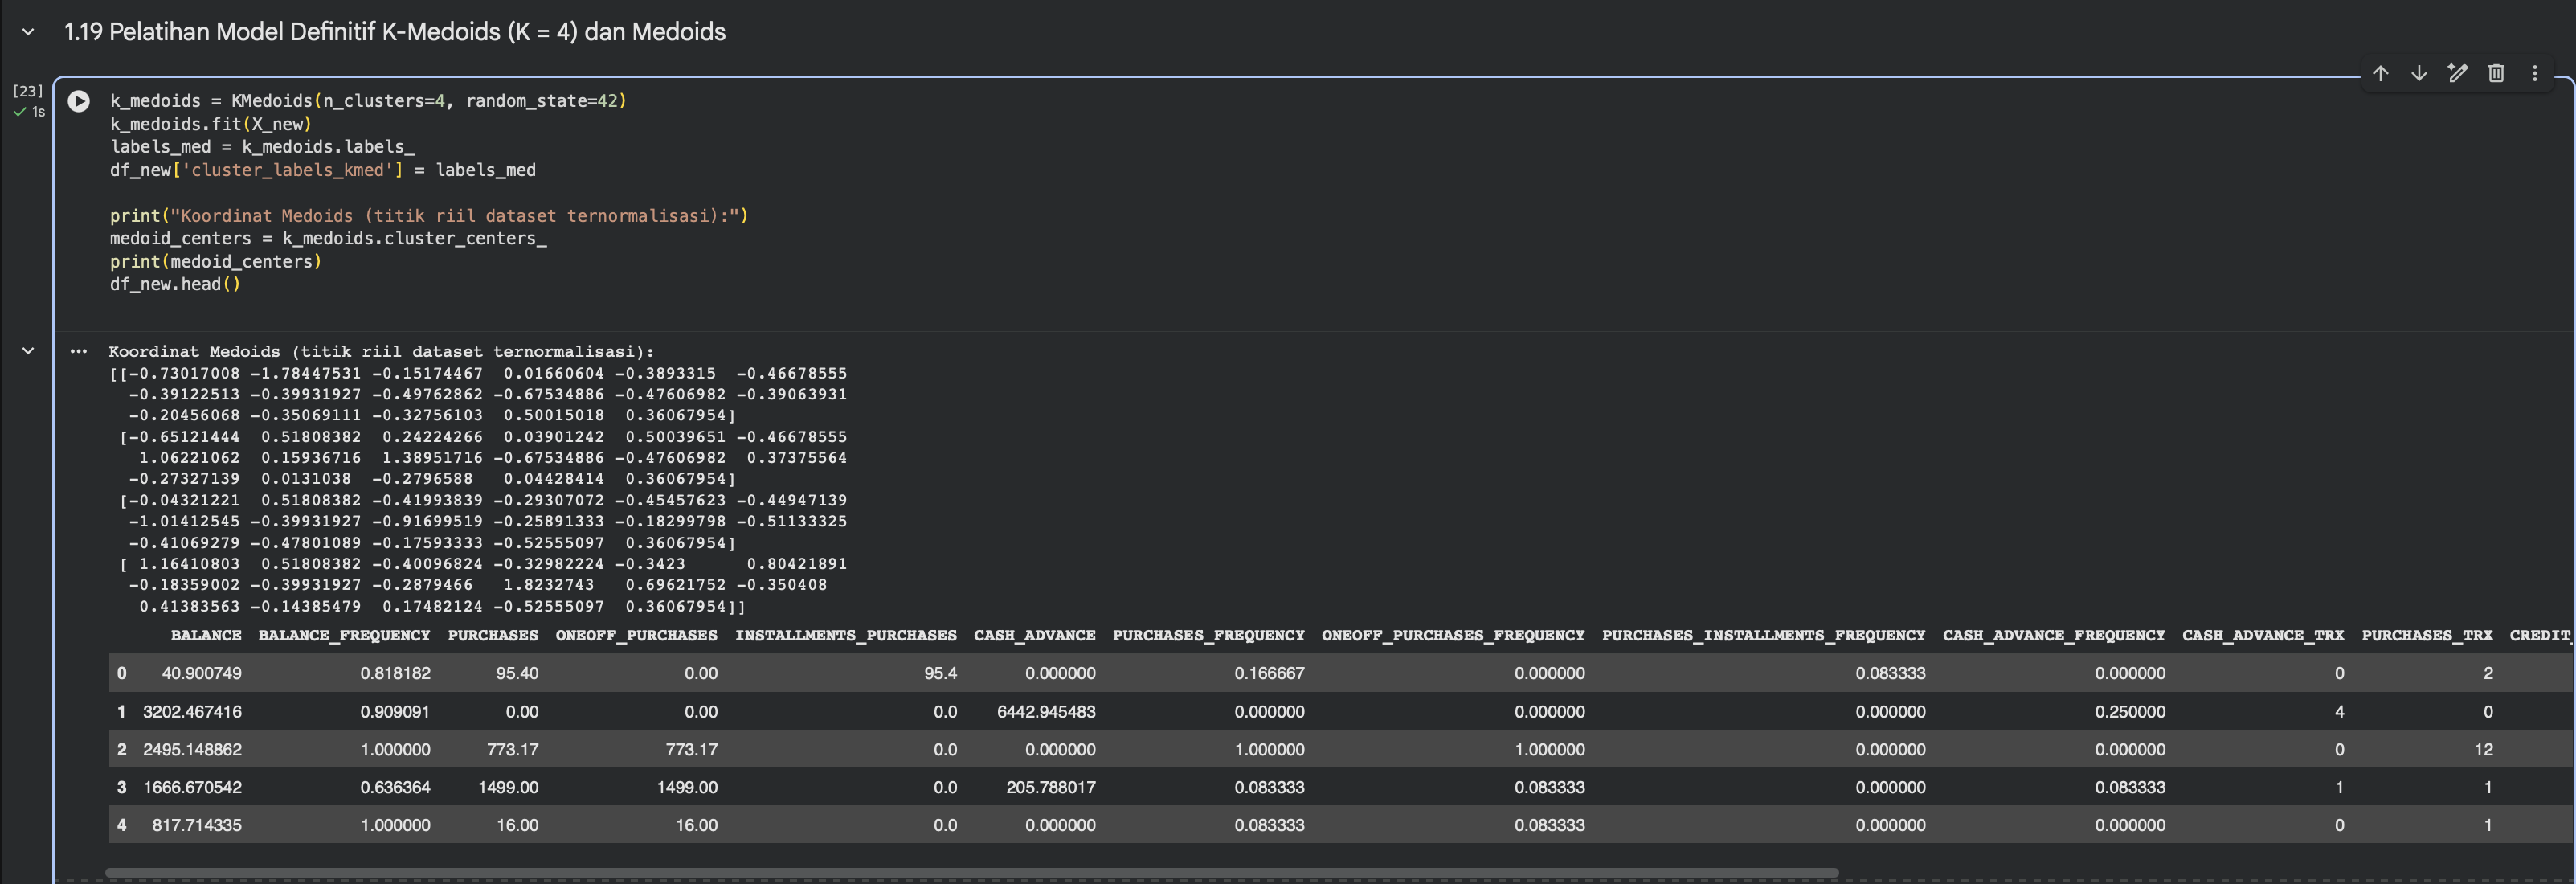
\includegraphics[width=0.8\textwidth]{images/ss-26-train-kmedoids.png}}
\caption{Tangkapan layar pelatihan K-Medoids K = 4.}
\label{fig:ss-train-kmedoids}
\end{figure}

\begin{figure}[H]
\centering
\begin{minipage}[b]{0.48\textwidth}
    \centering
    \customfbox{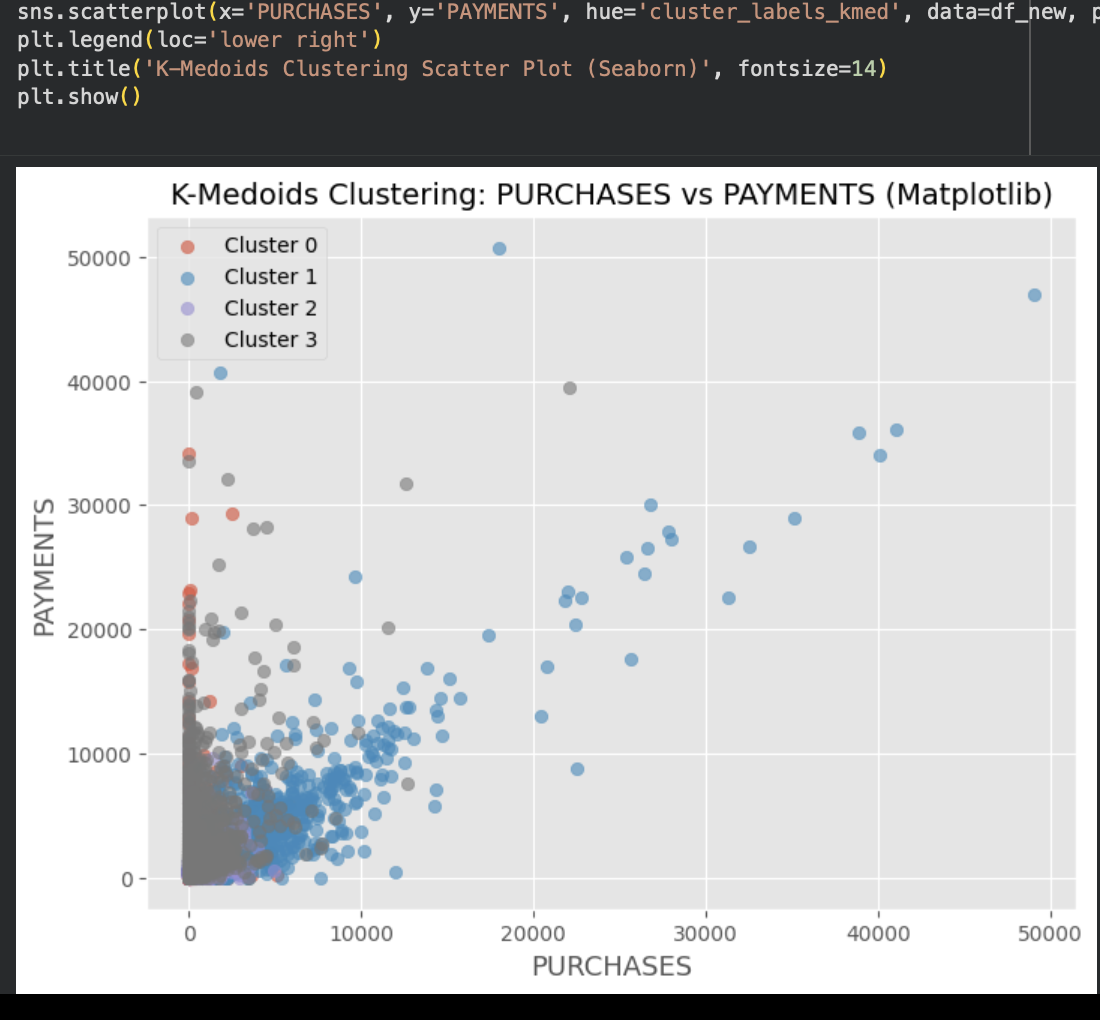
\includegraphics[width=\dimexpr\linewidth-1pt\relax]{images/ss-27-scatter-matplotlib-kmedoids.png}}
    \caption{Visualisasi 2D K-Medoids (Matplotlib).}
    \label{fig:ss-scatter-matplotlib-kmedoids}
\end{minipage}
\hfill
\begin{minipage}[b]{0.48\textwidth}
    \centering
    \customfbox{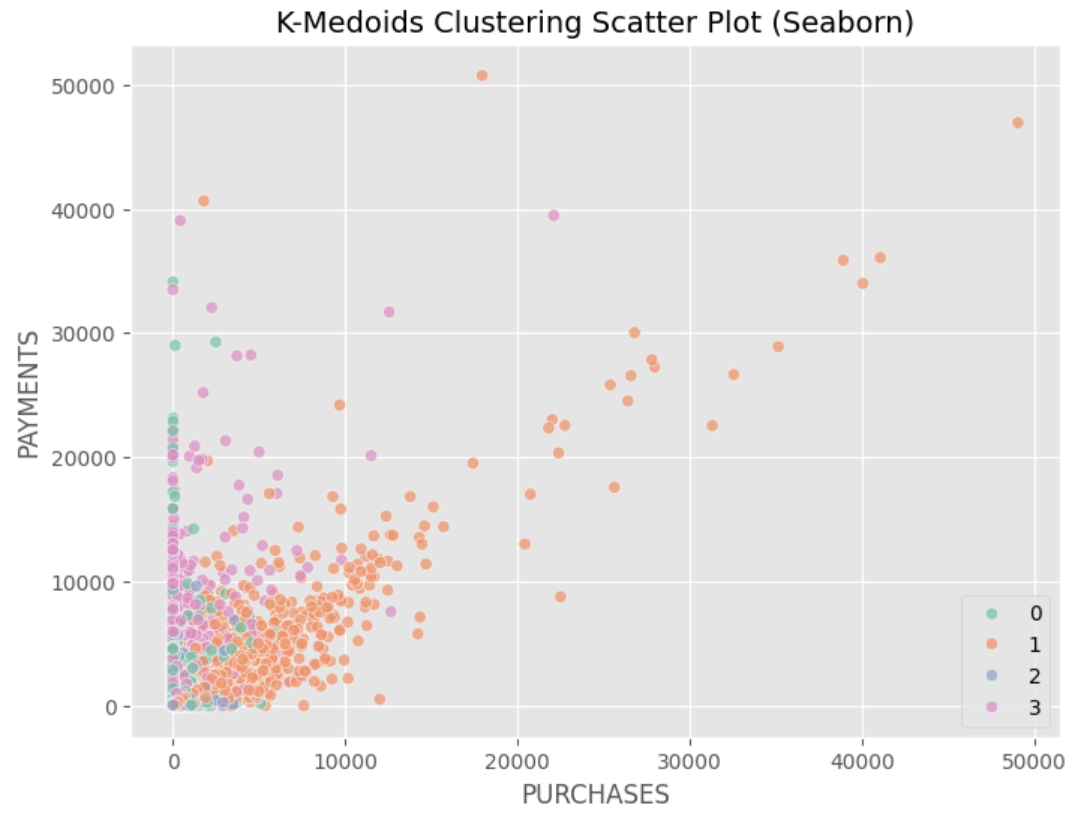
\includegraphics[width=\dimexpr\linewidth-1pt\relax]{images/ss-28-scatter-seaborn-kmedoids.png}}
    \caption{Visualisasi 2D K-Medoids (Seaborn).}
    \label{fig:ss-scatter-seaborn-kmedoids}
\end{minipage}
\end{figure}

\subsection{Analisis Profil Klaster dan Interpretasi Bisnis}
Untuk menafsirkan makna perilaku tiap klaster K-Means ($K = 4$), saya melakukan agregasi rata-rata dan total nilai pada fitur-fitur finansial utama.

\begin{lstlisting}[style=pythonstyle,caption={Agregasi rata-rata fitur per klaster.}]
df_out = df_new.groupby('cluster_labels').mean().reset_index()
cols = ['cluster_labels', 'BALANCE', 'PURCHASES',
        'PAYMENTS', 'CASH_ADVANCE', 'CREDIT_LIMIT']
df_out[cols]
\end{lstlisting}

\begin{figure}[H]
\centering
\customfbox{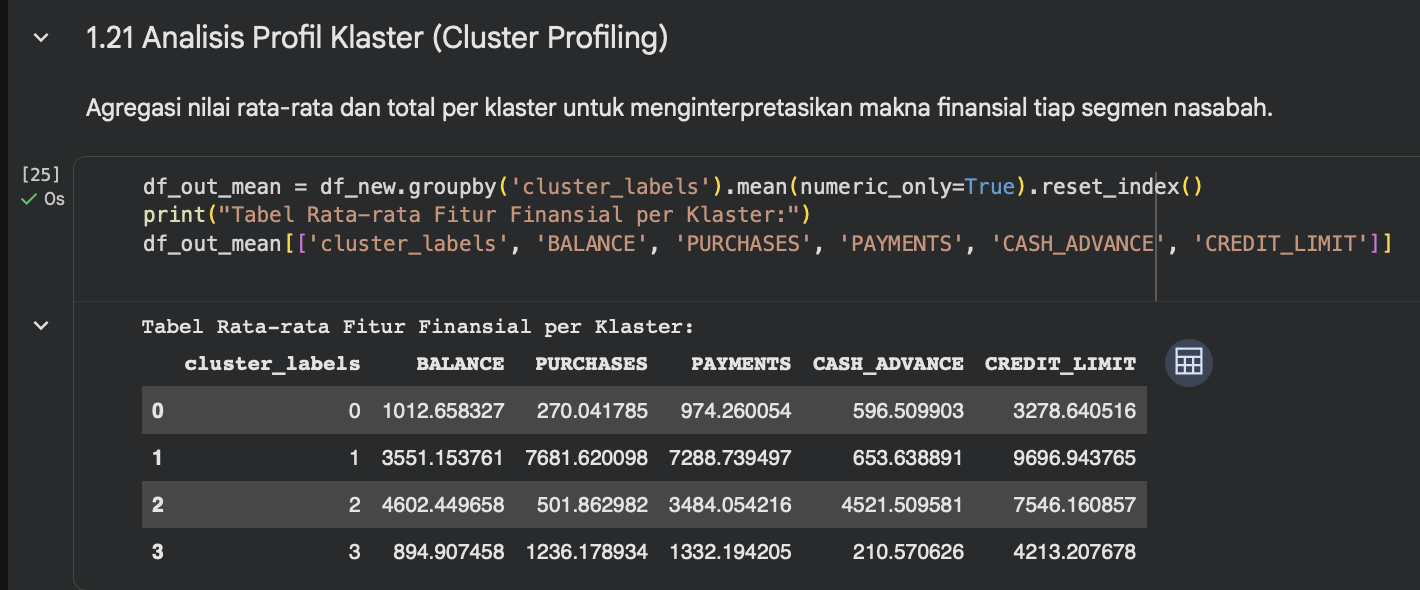
\includegraphics[width=0.65\textwidth]{images/ss-29-tabel-profiling.png}}
\caption{Tangkapan layar tabel agregasi rata-rata fitur per klaster.}
\label{fig:ss-tabel-profiling}
\end{figure}

Hasil agregasi fitur finansial dirangkum pada Tabel~\ref{tab:karakteristik-klaster}.

\begin{table}[H]
\centering
\small
\setlength{\tabcolsep}{3.2pt}
\begin{tabular}{cccccc}
\toprule
\textbf{Klaster} & \textbf{BALANCE} & \textbf{PURCHASES} & \textbf{PAYMENTS} & \textbf{CASH\_ADVANCE} & \textbf{CREDIT\_LIMIT} \\
\midrule
Cluster 0 & \$1.012{,}66 & \$270{,}04 & \$974{,}26 & \$596{,}51 & \$3.278{,}64 \\
Cluster 1 & \$3.551{,}15 & \$7.681{,}62 & \$7.288{,}74 & \$653{,}64 & \$9.696{,}94 \\
Cluster 2 & \$4.602{,}45 & \$501{,}86 & \$3.484{,}05 & \$4.521{,}51 & \$7.546{,}16 \\
Cluster 3 & \$894{,}91 & \$1.236{,}18 & \$1.332{,}19 & \$210{,}57 & \$4.213{,}21 \\
\bottomrule
\end{tabular}
\caption{Rata-rata fitur finansial pada keempat klaster hasil K-Means ($K = 4$).}
\label{tab:karakteristik-klaster}
\end{table}

Saya juga memvisualisasikan diagram batang perbandingan tiga variabel utama antar-klaster.

\begin{lstlisting}[style=pythonstyle,caption={Diagram batang perbandingan fitur utama antar-klaster.}]
plt.figure(figsize=(18, 4))
plt.subplot(1, 3, 1)
sns.barplot(x='cluster_labels', y='PURCHASES', data=df_out)
plt.title('Rata-rata PURCHASES')

plt.subplot(1, 3, 2)
sns.barplot(x='cluster_labels', y='PAYMENTS', data=df_out)
plt.title('Rata-rata PAYMENTS')

plt.subplot(1, 3, 3)
sns.barplot(x='cluster_labels', y='BALANCE', data=df_out)
plt.title('Rata-rata BALANCE')
plt.show()
\end{lstlisting}

\begin{figure}[H]
\centering
\customfbox{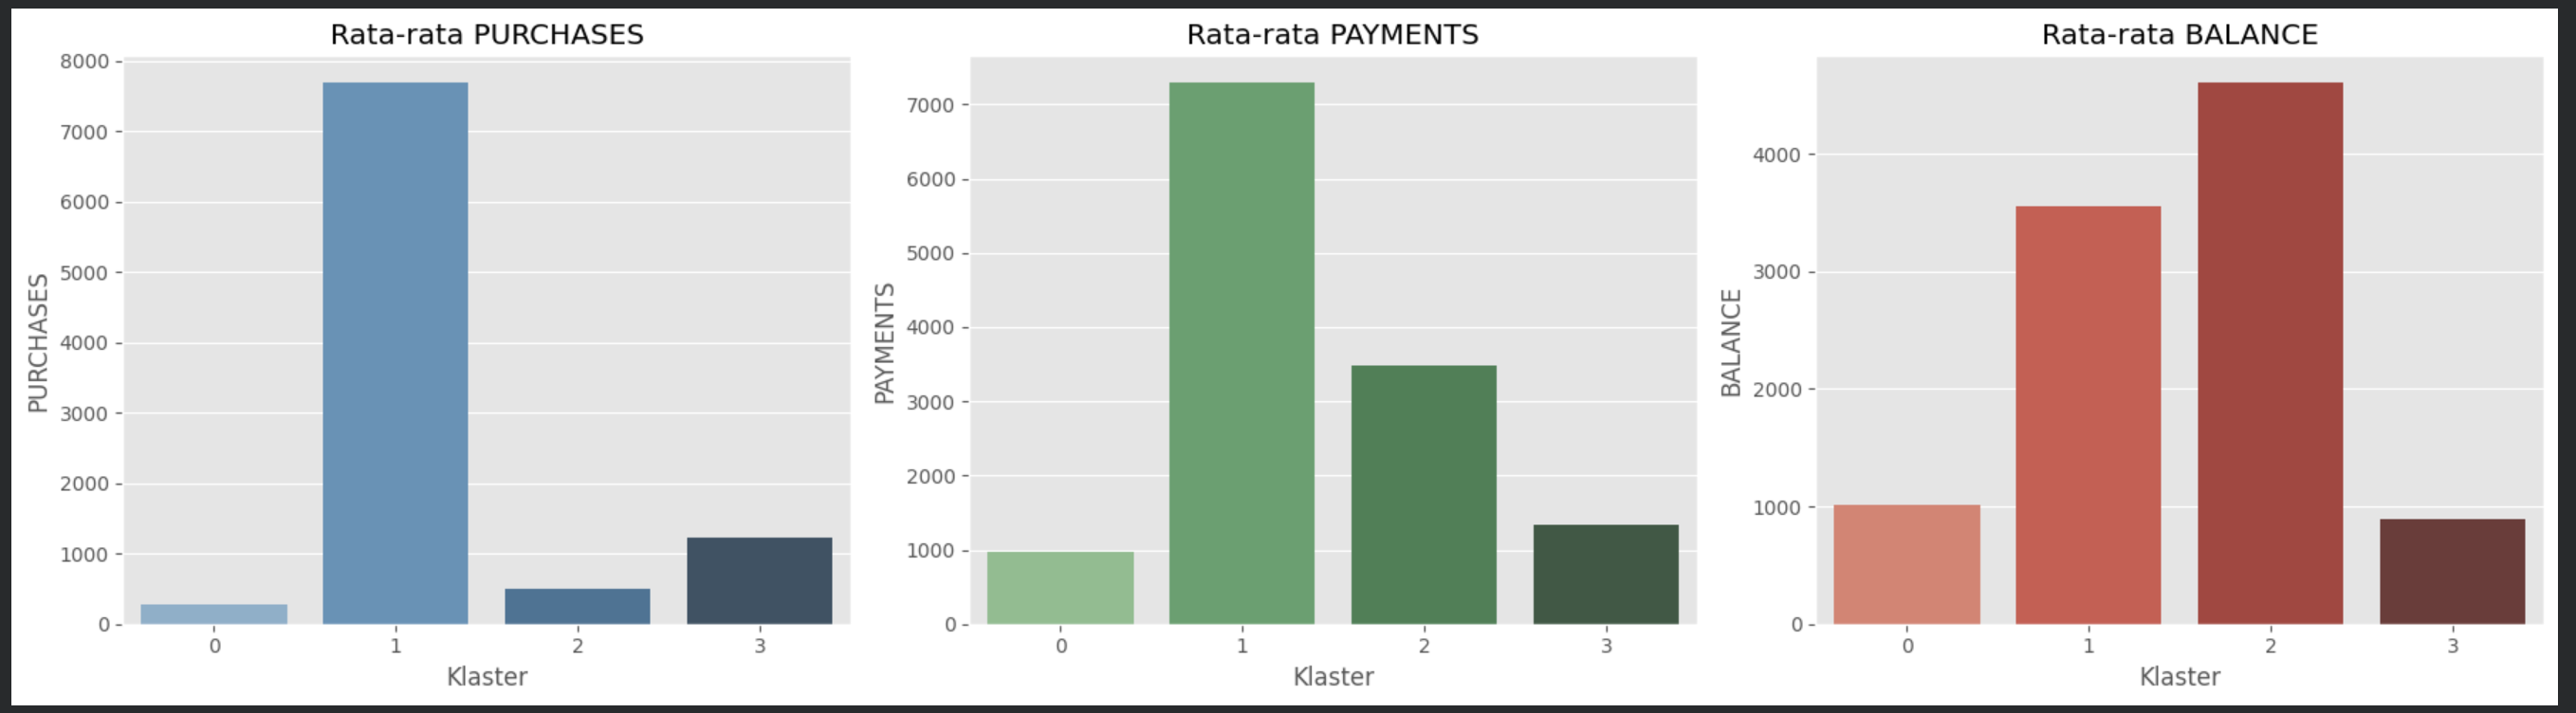
\includegraphics[width=0.72\textwidth]{images/ss-30-barplot-profiling.png}}
\caption{Tangkapan layar diagram batang perbandingan rata-rata pembelian, pembayaran, dan saldo.}
\label{fig:ss-barplot-profiling}
\end{figure}

Berdasarkan nilai rata-rata dan pola perilakunya, keempat kelompok nasabah diklasifikasikan sebagai berikut:
\begin{enumerate}[noitemsep, topsep=1pt, parsep=0.5pt, partopsep=0pt]
    \item \textbf{Cluster 0 (Nasabah Inaktif / Saldo Rendah):} Nilai rata-rata pembelian (\$270) dan pembayaran tagihan (\$974) berada pada tingkat terendah, dengan saldo sekitar \$1.012 dan limit kredit \$3.278. Nasabah pada kelompok ini jarang memanfaatkan kartu kredit. Strategi bisnis yang direkomendasikan adalah penawaran program bebas iuran tahunan (\textit{annual fee waiver}), diskon transaksi pertama pada merchant rekanan, serta pengiriman notifikasi berkala untuk mendorong pemakaian kartu.
    \item \textbf{Cluster 1 (Nasabah Belanja VIP / Pengeluaran Tinggi):} Menunjukkan rata-rata pembelian tertinggi (\$7.681) dan pembayaran tertinggi (\$7.288) dengan limit kredit terbesar (\$9.696). Nasabah kelompok ini berdaya beli sangat tinggi dan melunasi tagihan secara tertib. Strategi bisnis yang tepat meliputi kenaikan pagu kredit berkala, penawaran peningkatan status kartu ke tier premium (Platinum atau World Elite), serta penyediaan fasilitas \textit{airport lounge} dan asuransi proteksi perjalanan.
    \item \textbf{Cluster 2 (Nasabah Saldo Tinggi / Pengguna Fasilitas Dana Tunai):} Memiliki saldo utang tertinggi (\$4.602) dan penarikan uang tunai tertinggi (\$4.521) dengan nominal pembayaran tagihan \$3.484. Kelompok ini mempertahankan saldo utang bergulir dan rutin memakai fasilitas tarik tunai ATM. Segmen ini menghasilkan marjin pendapatan bunga yang signifikan bagi bank, tetapi memiliki profil risiko kredit lebih besar. Bank dapat menawarkan restrukturisasi saldo menjadi skema cicilan tetap dengan suku bunga kompetitif guna menekan potensi gagal bayar (\textit{default}).
    \item \textbf{Cluster 3 (Nasabah Transaksi Rutin / Pengeluaran Moderat):} Menunjukkan nilai pembelian (\$1.236), pembayaran (\$1.332), dan saldo (\$895) pada proporsi yang seimbang, dengan rasio penarikan dana tunai yang sangat minim (\$210). Nasabah memakai kartu secara tertib untuk berbelanja kebutuhan operasional bulanan. Strategi bisnis difokuskan pada program reward poin loyalitas dan fasilitas cicilan bunga 0\% pada merchant supermarket atau bahan bakar.
\end{enumerate}


\clearpage

\section{Tugas dan Analisis Praktikum}

\subsection{Soal 1: Dataset Preparation (Credit Card Dataset)}
Dataset kartu kredit diunduh dari repositori Kaggle pada tautan:
\begin{center}
\href{https://www.kaggle.com/datasets/arjunbhasin2013/ccdata}{\textcolor{blue}{https://www.kaggle.com/datasets/arjunbhasin2013/ccdata}} \cite{kaggle-ccdata}
\end{center}

\subsubsection{Tujuan Penggunaan Dataset}
Dataset ini dikembangkan untuk membangun segmentasi nasabah kartu kredit berbasis perilaku transaksi. Melalui segmentasi ini, perbankan dapat:
\begin{enumerate}[noitemsep, topsep=2pt, parsep=1pt]
    \item Menyesuaikan program pemasaran kartu kredit dengan preferensi belanja nasabah.
    \item Mengelola risiko kredit secara terukur dengan menetapkan batas limit kredit yang sesuai dengan kemampuan bayar.
    \item Mengurangi rasio nasabah berhenti memakai layanan (customer churn) dengan memberikan insentif retensi yang relevan bagi nasabah yang jarang bertransaksi.
\end{enumerate}

\subsubsection{Deskripsi dan Makna Fitur Dataset}
Dataset memuat 18 fitur yang mencakup perilaku transaksi nasabah selama periode observasi enam bulan. Rincian seluruh fitur disajikan pada Tabel~\ref{tab:deskripsi-fitur-cc}.

\begin{table}[htbp]
\centering
\scriptsize
\renewcommand{\arraystretch}{0.88}
\begin{tabularx}{\textwidth}{p{0.5cm} p{4.0cm} p{1.3cm} >{\raggedright\arraybackslash}X}
\toprule
\textbf{No} & \textbf{Nama Fitur} & \textbf{Tipe Data} & \textbf{Deskripsi dan Makna Operasional} \\
\midrule
1 & \texttt{CUST\_ID} & String & Nomor identitas unik pemegang kartu kredit (kategorikal murni, tidak digunakan). \\
2 & \texttt{BALANCE} & Float & Jumlah saldo utang yang masih tersisa pada rekening kartu kredit nasabah. \\
3 & \texttt{BALANCE\_FREQUENCY} & Float & Rasio keteraturan pembaruan saldo berkala (skor 0 sampai 1). \\
4 & \texttt{PURCHASES} & Float & Total akumulasi nominal pembelanjaan nasabah selama 6 bulan observasi. \\
5 & \texttt{ONEOFF\_PURCHASES} & Float & Total transaksi belanja yang dibayar tunai langsung tanpa skema cicilan. \\
6 & \texttt{INSTALLMENTS\_PURCHASES} & Float & Total transaksi belanja yang dibayar melalui skema cicilan bertahap. \\
7 & \texttt{CASH\_ADVANCE} & Float & Total dana tunai yang ditarik nasabah di muka melalui mesin ATM. \\
8 & \texttt{PURCHASES\_FREQUENCY} & Float & Frekuensi transaksi pembelian belanja nasabah (skor 0 sampai 1). \\
9 & \texttt{ONEOFF\_PURCHASES\_}\newline\texttt{FREQUENCY} & Float & Frekuensi transaksi belanja tunai sekaligus (skor 0 sampai 1). \\
10 & \texttt{PURCHASES\_INSTALLMENTS\_}\newline\texttt{FREQUENCY} & Float & Frekuensi transaksi belanja dengan metode cicilan (skor 0 sampai 1). \\
11 & \texttt{CASH\_ADVANCE\_FREQUENCY} & Float & Frekuensi transaksi penarikan uang tunai di muka (skor 0 sampai 1). \\
12 & \texttt{CASH\_ADVANCE\_TRX} & Integer & Total frekuensi hitungan transaksi penarikan dana tunai di muka. \\
13 & \texttt{PURCHASES\_TRX} & Integer & Total hitungan kuantitas transaksi pembelian yang dilakukan nasabah. \\
14 & \texttt{CREDIT\_LIMIT} & Float & Batas pagu kredit maksimum yang dialokasikan oleh penerbit kartu. \\
15 & \texttt{PAYMENTS} & Float & Total akumulasi nominal pembayaran tagihan yang telah disetorkan. \\
16 & \texttt{MINIMUM\_PAYMENTS} & Float & Total nominal pembayaran minimum untuk menjaga kartu tetap aktif. \\
17 & \texttt{PRC\_FULL\_PAYMENT} & Float & Persentase tagihan kartu kredit yang dilunasi penuh (100\%) setiap bulan. \\
18 & \texttt{TENURE} & Integer & Masa kepemilikan kartu kredit oleh nasabah (rentang 6 sampai 12 bulan). \\
\bottomrule
\end{tabularx}
\caption{Deskripsi lengkap 18 fitur pada Credit Card Dataset.}
\label{tab:deskripsi-fitur-cc}
\end{table}


\subsection{Soal 2: Eksperimen Klasterisasi Dataset Air Traffic Passenger Statistics}
Sesuai arahan tugas praktikum, eksperimen klasterisasi mandiri dijalankan memakai dataset operasional penerbangan yang bersumber dari portal data terbuka resmi Pemerintah Kota San Francisco (DataSF):
\begin{center}
\url{https://data.sfgov.org/Transportation/Air-Traffic-Passenger-Statistics/rkru-6vcg/about_data} \cite{sfgov-airtraffic}
\end{center}

Dataset mencatat statistik lalu lintas penumpang bulanan di Bandara Internasional San Francisco (SFO). Fitur di dalamnya memuat identitas maskapai penerbangan (\texttt{Operating Airline}), cakupan wilayah (\texttt{GEO Summary} dan \texttt{GEO Region}), jenis aktivitas penumpang (\texttt{Activity Type Description}), kategori harga layanan (\texttt{Price Category Code}), terminal keberangkatan/kedatangan (\texttt{Terminal} dan \texttt{Boarding Area}), serta jumlah penumpang (\texttt{Passenger Count}).

\subsubsection{Pemrosesan Data dan Pengkodean Kategori}
Fitur teks pada dataset penerbangan ditransformasikan menjadi representasi numerik menggunakan \texttt{LabelEncoder} dari pustaka \texttt{sklearn.preprocessing}.

\begin{lstlisting}[style=pythonstyle,caption={Pemuatan data dan pengkodean fitur kategori dengan LabelEncoder.}]
import pandas as pd
import numpy as np
from sklearn.preprocessing import LabelEncoder, StandardScaler
from sklearn.cluster import KMeans
from sklearn_extra.cluster import KMedoids
from sklearn.metrics import silhouette_score
from kneed import KneeLocator

df_air = pd.read_csv('Air_Traffic_Passenger_Statistics.csv')
print("Dimensi dataset penerbangan:", df_air.shape)

cats = df_air.select_dtypes(include=['object', 'bool']).columns
cat_features = list(cats.values)

le = LabelEncoder()
for col in cat_features:
    df_air[col] = le.fit_transform(df_air[col].astype(str))

df_air.head()
\end{lstlisting}

\begin{figure}[H]
\centering
\customfbox{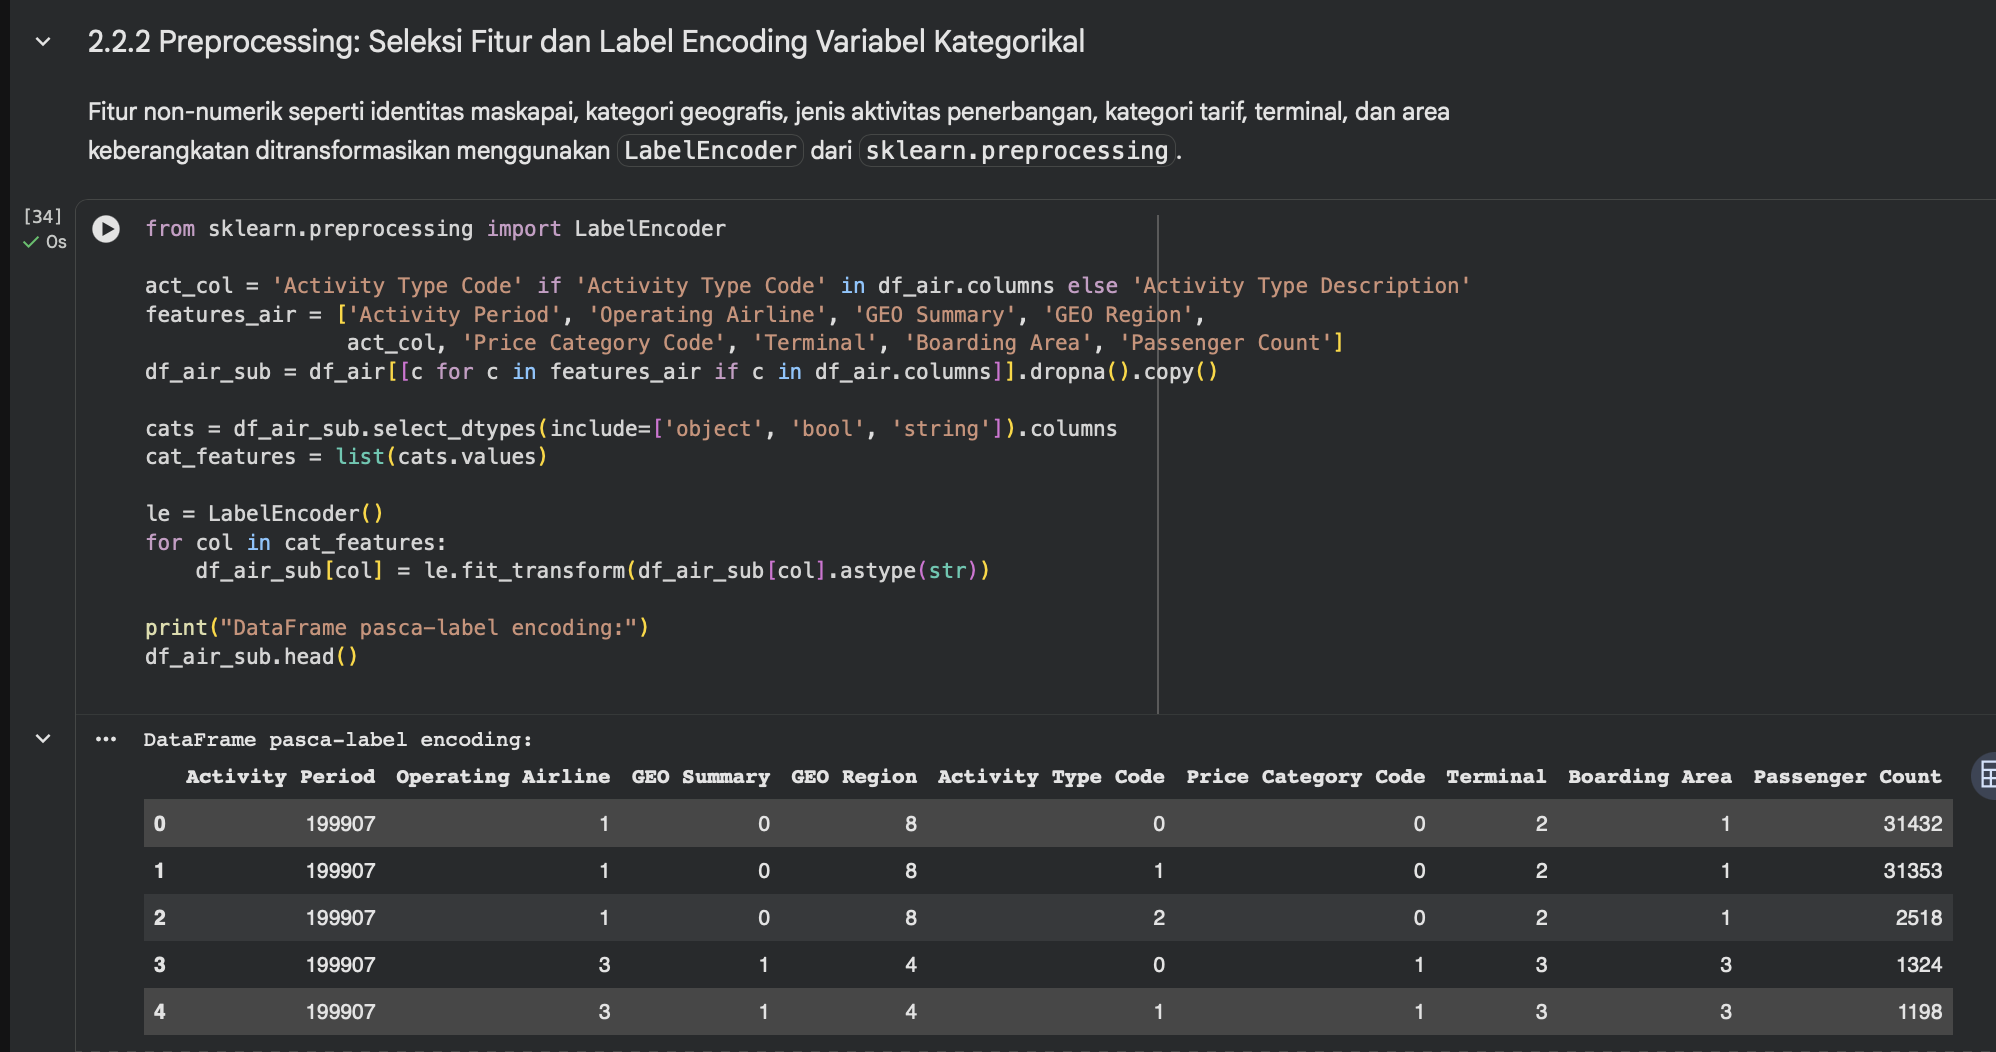
\includegraphics[width=0.75\textwidth]{images/ss-31-tugas-air-load.png}}
\caption{Tangkapan layar pemuatan dataset dan transformasi LabelEncoder pada data penerbangan.}
\label{fig:ss-tugas-air-load}
\end{figure}

Setelah dilakukan pengkodean, seluruh fitur numerik distandarisasi memakai \texttt{StandardScaler} agar memiliki rata-rata nol dan variansi satu.

\begin{lstlisting}[style=pythonstyle,caption={Standarisasi matriks fitur penerbangan.}]
X_air = df_air.values
scaler_air = StandardScaler()
X_air_scaled = scaler_air.fit_transform(X_air)
\end{lstlisting}

\begin{figure}[H]
\centering
\customfbox{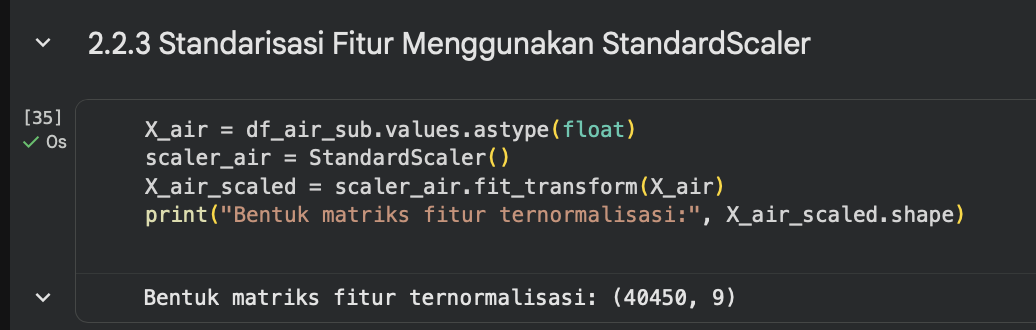
\includegraphics[width=0.7\textwidth]{images/ss-32-tugas-air-scaling.png}}
\caption{Tangkapan layar standarisasi matriks fitur penerbangan.}
\label{fig:ss-tugas-air-scaling}
\end{figure}

\subsubsection{Penentuan Nilai K Optimal pada Data Penerbangan}
Saya menguji variasi nilai $K = 1$ hingga $10$ memakai K-Means dan K-Medoids dengan menghitung Inertia serta Silhouette Score.

\begin{lstlisting}[style=pythonstyle,caption={Evaluasi Elbow Method dan Silhouette Score data penerbangan.}]
inertia_air_kmeans = []
silhouette_air_kmeans = []

for k in range(1, 11):
    km = KMeans(n_clusters=k, random_state=42)
    km.fit(X_air_scaled)
    inertia_air_kmeans.append(km.inertia_)
    if k >= 2:
        score = silhouette_score(X_air_scaled, km.labels_)
        silhouette_air_kmeans.append(score)

kneedle_air = KneeLocator(
    range(1, 11), inertia_air_kmeans,
    curve='convex', direction='decreasing'
)
print("Optimal K (K-Means):", kneedle_air.knee)
\end{lstlisting}

\begin{figure}[H]
\centering
\begin{minipage}[b]{0.48\textwidth}
    \centering
    \customfbox{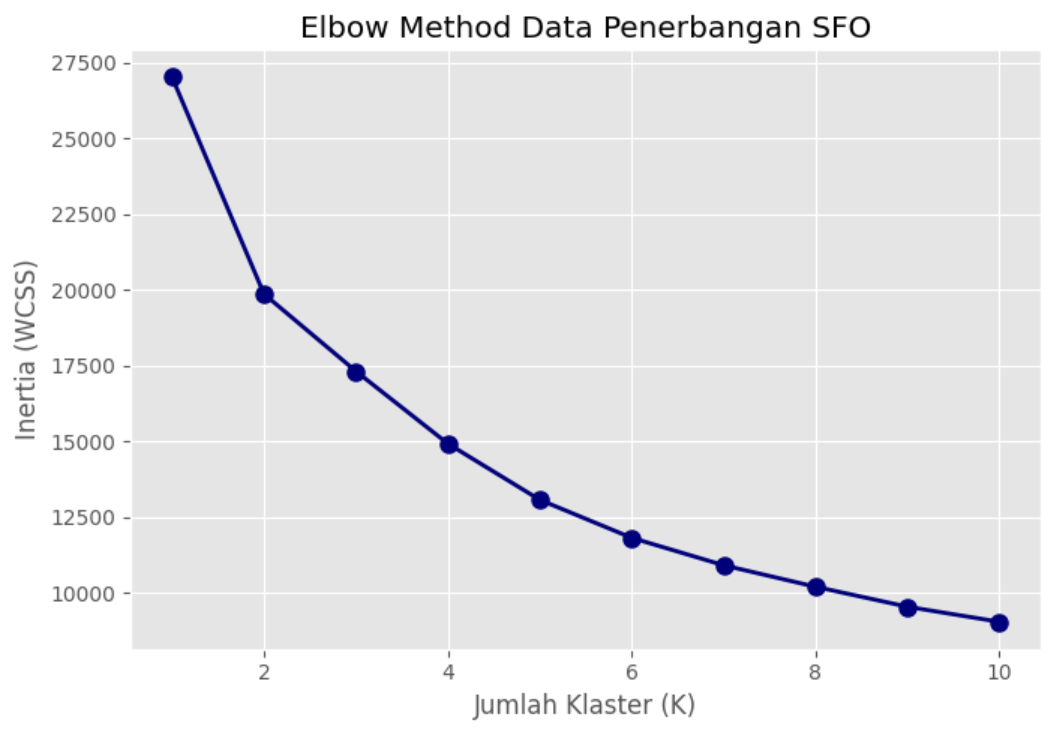
\includegraphics[width=\dimexpr\linewidth-1pt\relax]{images/ss-33-tugas-air-elbow.png}}
    \caption{Penurunan inertia penerbangan.}
    \label{fig:ss-tugas-air-elbow}
\end{minipage}
\hfill
\begin{minipage}[b]{0.48\textwidth}
    \centering
    \customfbox{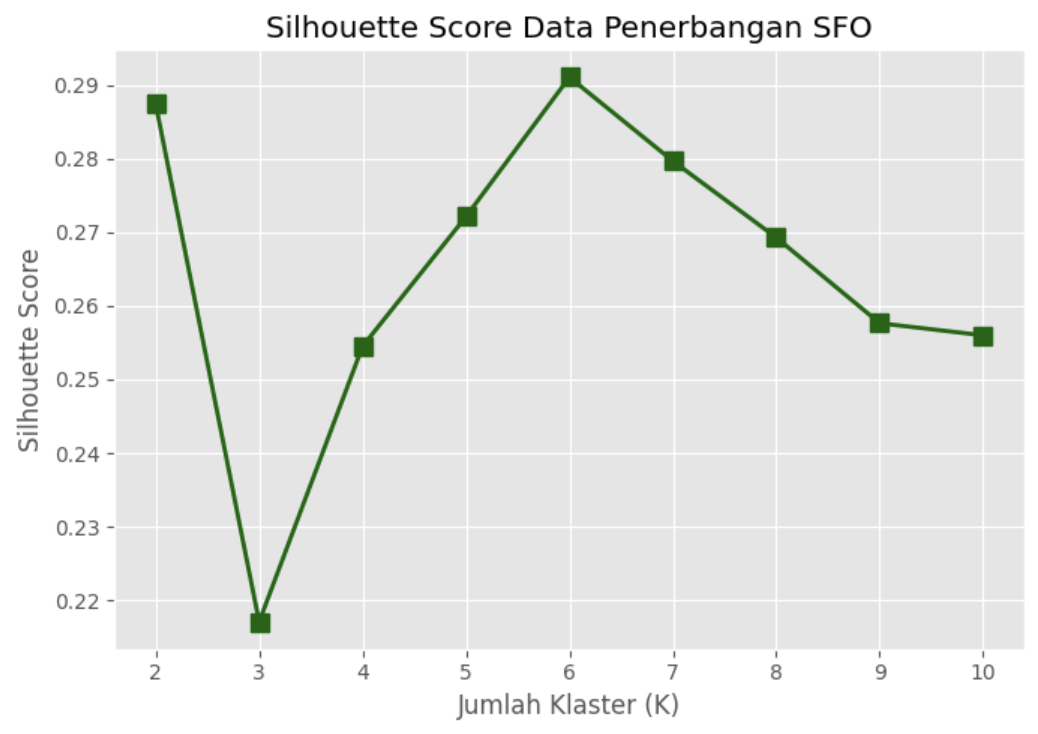
\includegraphics[width=\dimexpr\linewidth-1pt\relax]{images/ss-34-tugas-air-sil.png}}
    \caption{Silhouette Score penerbangan.}
    \label{fig:ss-tugas-air-sil}
\end{minipage}
\end{figure}

Hasil pengujian kurva inertia memperlihatkan kelokan siku kurva pada $K = 4$. Silhouette score menunjukkan nilai yang relatif stabil pada rentang $K = 3$ dan $K = 4$. Nilai $K = 4$ dipilih karena membagi struktur operasional penerbangan bandara secara seimbang ke dalam empat kelompok yang terpisah dengan jelas.

\subsubsection{Penerapan K-Means dan K-Medoids}
Kedua model klasterisasi dilatih memakai nilai $K = 4$.

\begin{lstlisting}[style=pythonstyle,caption={Pelatihan K-Means dan K-Medoids pada data penerbangan.}]
kmeans_air = KMeans(n_clusters=4, random_state=42)
df_air['cluster_kmeans'] = kmeans_air.fit_predict(X_air_scaled)

kmedoids_air = KMedoids(n_clusters=4, random_state=42)
df_air['cluster_kmedoids'] = kmedoids_air.fit_predict(X_air_scaled)
\end{lstlisting}

\begin{figure}[H]
\centering
\customfbox{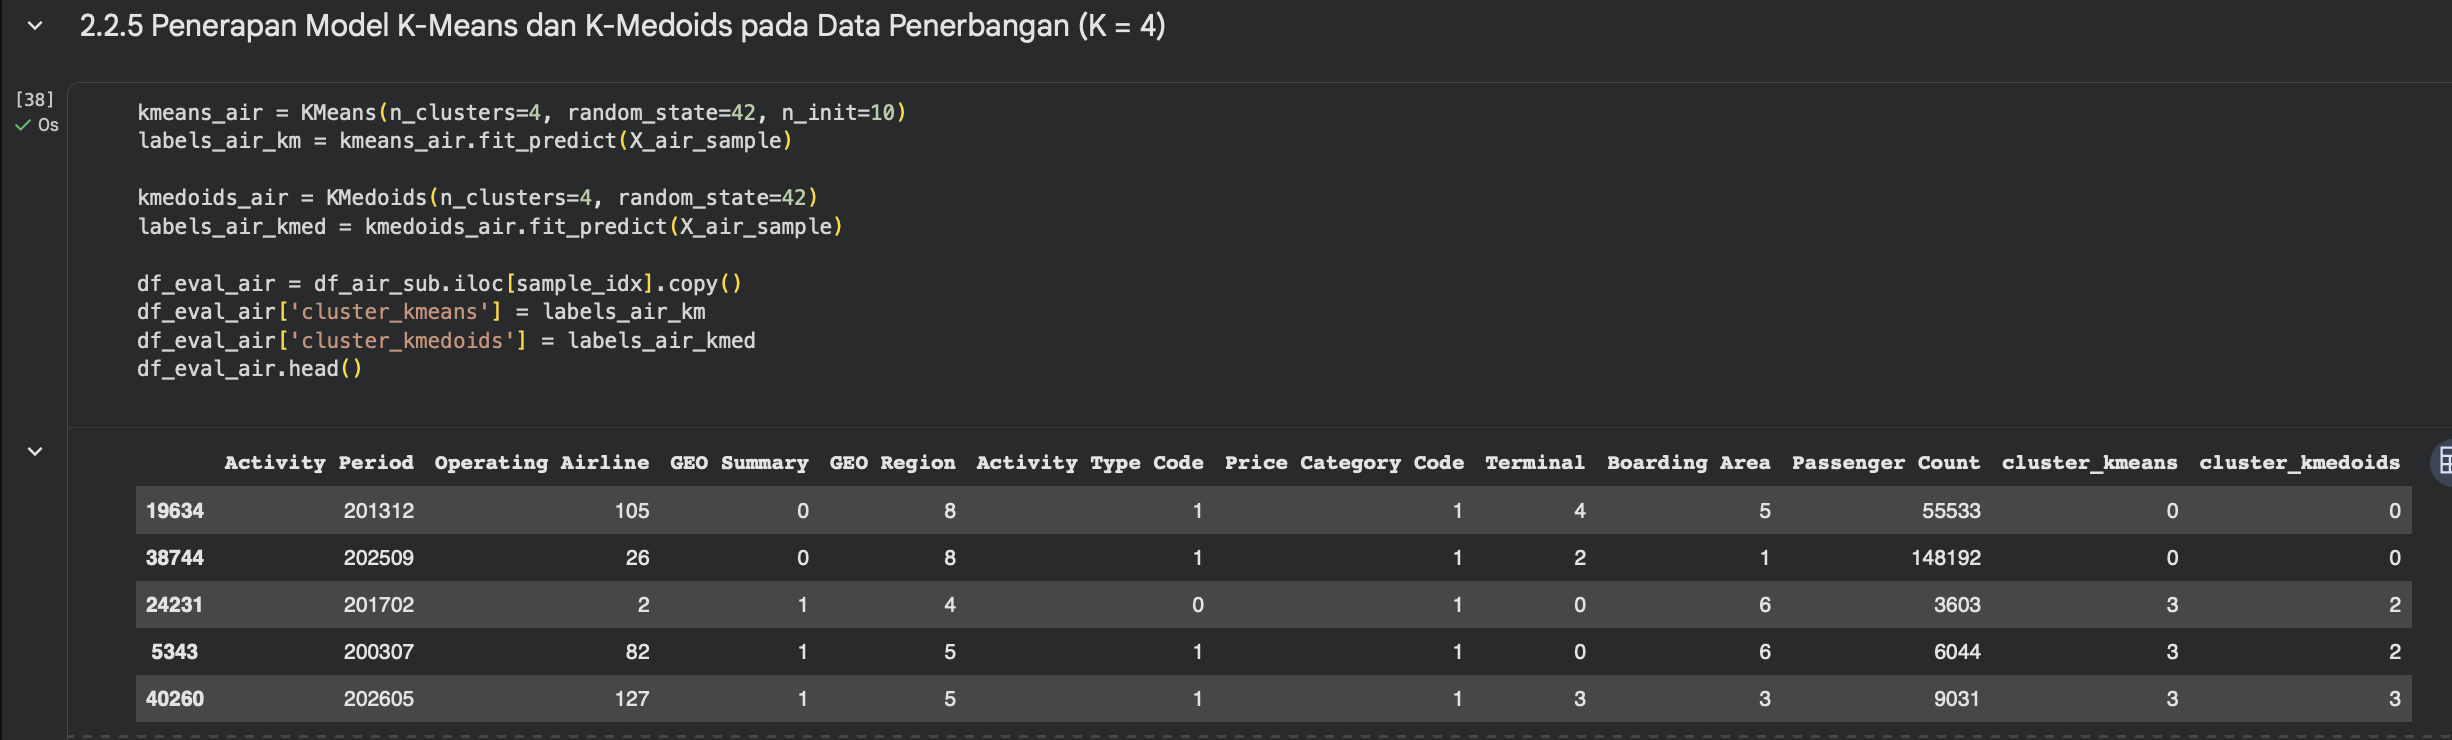
\includegraphics[width=0.75\textwidth]{images/ss-35-tugas-air-train.png}}
\caption{Tangkapan layar pelatihan K-Means dan K-Medoids pada data penerbangan.}
\label{fig:ss-tugas-air-train}
\end{figure}

\begin{figure}[H]
\centering
\begin{minipage}[b]{0.48\textwidth}
    \centering
    \customfbox{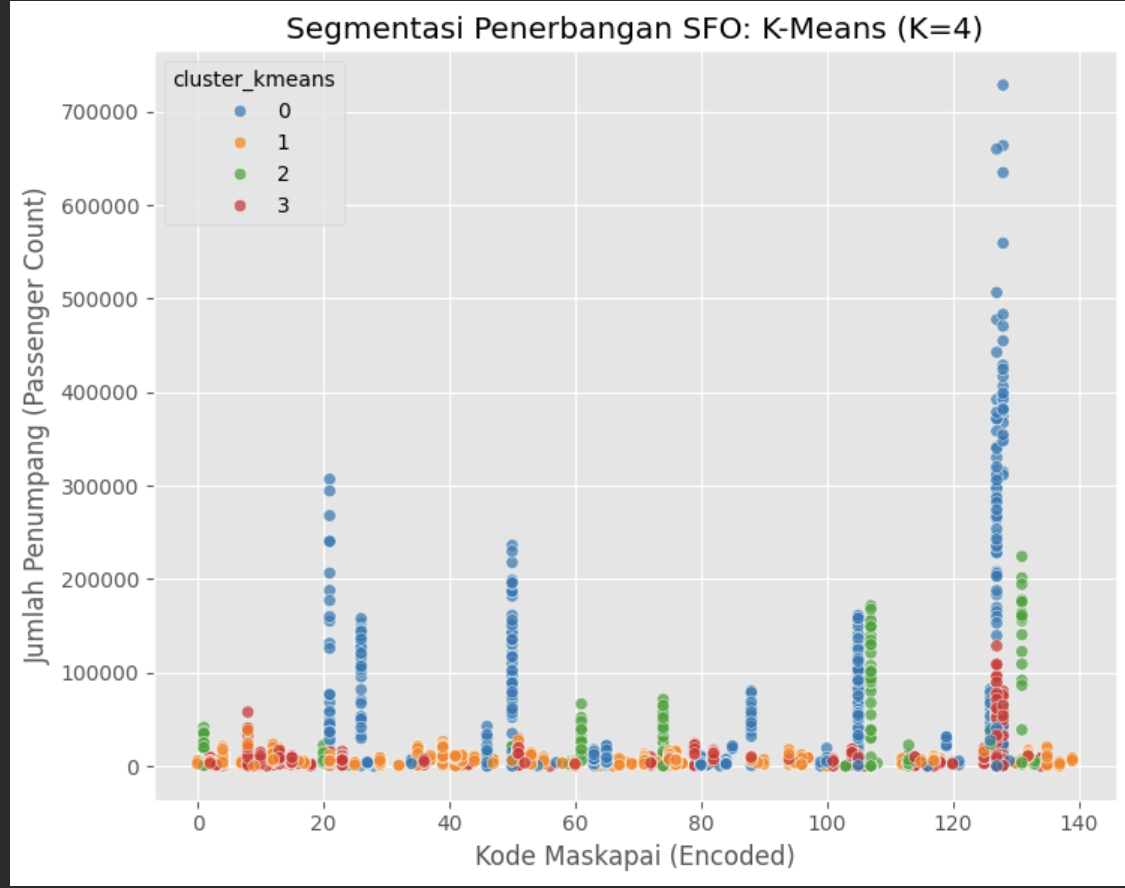
\includegraphics[width=\dimexpr\linewidth-1pt\relax]{images/ss-36-tugas-air-scatter-km.png}}
    \caption{Klaster 2D K-Means.}
    \label{fig:ss-tugas-air-scatter-km}
\end{minipage}
\hfill
\begin{minipage}[b]{0.48\textwidth}
    \centering
    \customfbox{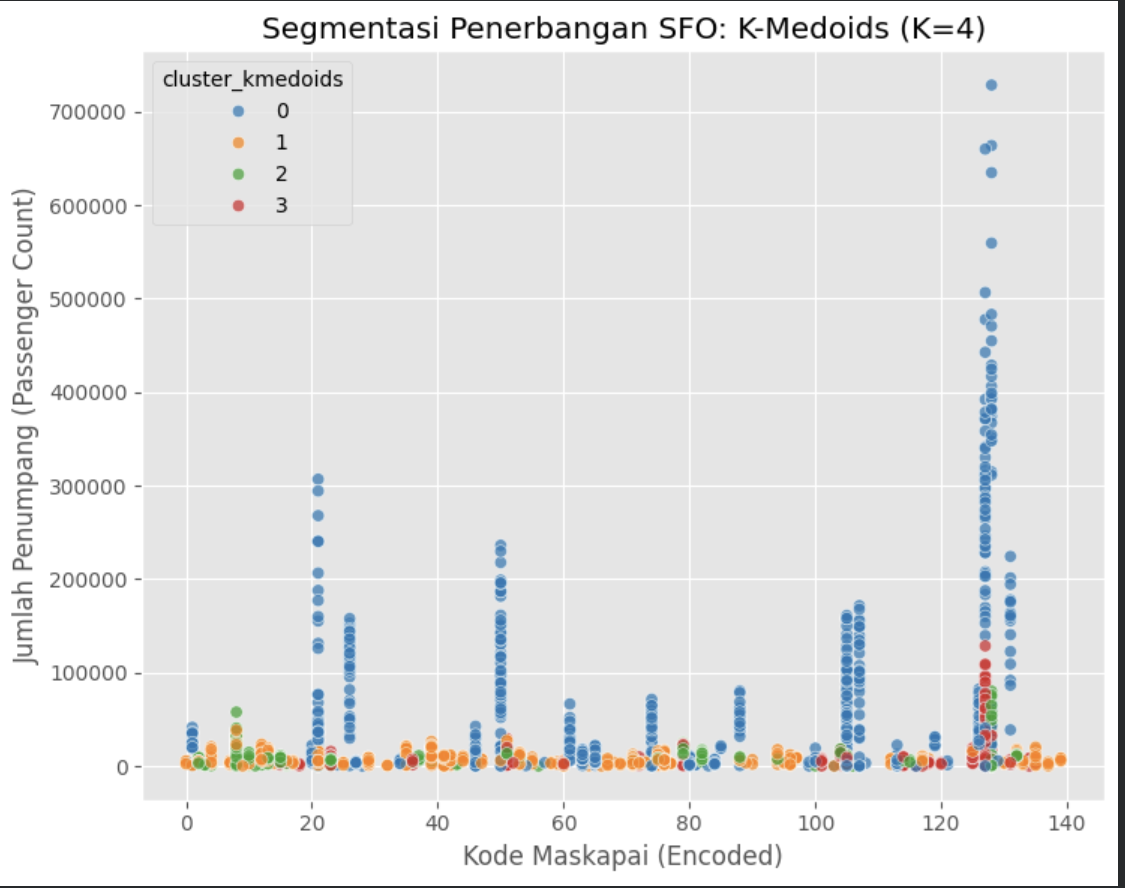
\includegraphics[width=\dimexpr\linewidth-1pt\relax]{images/ss-37-tugas-air-scatter-kmed.png}}
    \caption{Klaster 2D K-Medoids.}
    \label{fig:ss-tugas-air-scatter-kmed}
\end{minipage}
\end{figure}

Berdasarkan agregasi fitur operasional, empat kelompok operasional penerbangan terbentuk:
\begin{enumerate}[noitemsep, topsep=2pt, parsep=1pt]
    \item \textbf{Segmen 1 (Maskapai Hub Domestik Volume Sangat Tinggi):} Didominasi oleh operator utama bandara SFO (seperti United Airlines dan SkyWest) yang melayani penerbangan domestik berfrekuensi tinggi dengan volume ratusan ribu penumpang per bulan.
    \item \textbf{Segmen 2 (Maskapai Bertarif Rendah / Low-Cost Carriers):} Meliputi maskapai berbiaya hemat (seperti Southwest Airlines dan JetBlue) yang melayani rute domestik dan regional dengan volume penumpang menengah.
    \item \textbf{Segmen 3 (Maskapai Internasional Jarak Jauh):} Meliputi maskapai rute lintas benua berlayanan penuh (seperti Lufthansa, British Airways, Singapore Airlines, dan Cathay Pacific) dengan terminal keberangkatan internasional dan volume penumpang bulanan yang konsisten.
    \item \textbf{Segmen 4 (Penerbangan Regional, Musiman, dan Charter):} Kelompok penerbangan dengan frekuensi terbatas atau musiman dengan jumlah penumpang bulanan yang relatif rendah.
\end{enumerate}

\subsubsection[Analisis Ketahanan terhadap Outlier]{Analisis Ketahanan terhadap Outlier (K-Means vs K-Medoids)}
Data operasional penerbangan bandara memiliki sebaran nilai pencilan yang nyata. Sebagai contoh, United Airlines memegang posisi sebagai maskapai hub di Bandara SFO dengan pangsa operasional melebihi 40\% dari total lalu lintas bandara. Jumlah penumpang bulanan United Airlines dapat mencapai jutaan orang, sementara puluhan maskapai internasional lainnya hanya mencatatkan puluhan ribu penumpang per bulan.

Perbedaan mekanisme kedua algoritma dalam merespons pencilan:
\begin{itemize}[noitemsep, topsep=2pt, parsep=1pt]
    \item \textbf{K-Means dan Kerentanan Nilai Rata-rata:} K-Means menghitung centroid sebagai rata-rata aritmetika dari seluruh anggota kelompok. Karena jarak dikuadratkan dalam fungsi objektif WCSS, titik pencilan bervolume jutaan penumpang memberikan penalti kuadratik yang besar. Akibatnya, posisi centroid tertarik menjauh ke arah nilai ekstrem tersebut. Pergeseran ini merusak partisi klaster, menyebabkan sebaran kelompok mayoritas maskapai normal tertekan dan batas kelompok menjadi kurang representatif.
    \item \textbf{K-Medoids dan Ketahanan Titik Riil:} K-Medoids memilih objek data aktual di dalam dataset sebagai pusat kelompok (medoid) dan meminimalkan jumlah dissimilaritas absolut. Karena medoid diwajibkan berupa sampel nyata dan tidak memakai kuadrat galat, keberadaan pencilan ekstrem pada satu maskapai tidak serta merta menggeser medoid. Pada evaluasi fungsi biaya swapping ($S = E_{\text{baru}} - E_{\text{lama}}$), menukar medoid ke titik pencilan justru memperbesar total selisih jarak absolut terhadap titik data lainnya ($S \ge 0$). Pertukaran tersebut otomatis ditolak, sehingga medoid tetap bertahan pada titik yang mewakili mayoritas data normal.
\end{itemize}

Hasil perbandingan ini menunjukkan bahwa pada data operasional dengan variansi ekstrem dan pencilan alami seperti statistik lalu lintas bandara, K-Medoids memberikan partisi pusat kelompok yang lebih stabil dibandingkan K-Means.

\subsection{Soal 3: Verifikasi Komputasi Association Rule dan Prinsip Apriori}
Sebagai materi pelengkap pada modul Pertemuan 6 mengenai \textit{Market Basket Analysis}, saya memverifikasi komputasi matematis metrik aturan asosiasi ($X \rightarrow Y$) menggunakan Python pada lima transaksi keranjang belanja. Aturan yang diuji adalah $\{Milk, Vegetables\} \rightarrow \{Fruits\}$.

\begin{figure}[H]
\centering
\customfbox{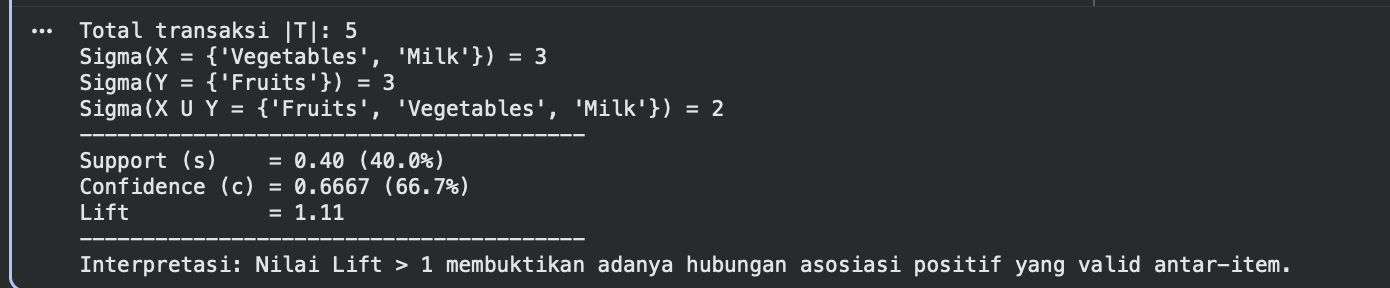
\includegraphics[width=0.75\textwidth]{images/ss-38-apriori-calc.png}}
\caption{Tangkapan layar hasil komputasi metrik Support, Confidence, dan Lift pada Google Colab.}
\label{fig:ss-apriori-calc}
\end{figure}

Hasil perhitungan pada Google Colab membuktikan:
\begin{enumerate}[noitemsep, topsep=2pt, parsep=1pt]
    \item \textbf{Support ($s = 0{,}40$):} Pasangan item $\{\text{Milk}, \text{Vegetables}, \text{Fruits}\}$ muncul bersamaan dalam 2 dari total 5 transaksi (40\%).
    \item \textbf{Confidence ($c = 0{,}6667$):} Dari 3 transaksi yang memuat $\{\text{Milk}, \text{Vegetables}\}$, sebanyak 2 transaksi juga membeli $\{\text{Fruits}\}$ (66{,}7\%).
    \item \textbf{Lift ($\mathit{Lift} = 1{,}11$):} Nilai Lift lebih besar dari 1 ($\mathit{Lift} > 1$) membuktikan bahwa kemunculan $\{\text{Fruits}\}$ bersama $\{\text{Milk}, \text{Vegetables}\}$ memiliki asosiasi positif nyata, bukan sekadar kebetulan independen.
\end{enumerate}


\clearpage

\chapter{Kesimpulan}
Berdasarkan praktikum yang telah saya laksanakan pada Pertemuan 6, diperoleh kesimpulan sebagai berikut:
\begin{enumerate}[noitemsep, topsep=2pt, parsep=0pt, partopsep=0pt]
    \item Unsupervised learning memodelkan struktur keteraturan pada data tanpa label target ($y$). Berbeda dengan supervised learning yang melatih fungsi prediksi berdasar acuan kebenaran (ground truth), unsupervised learning berfokus menemukan kelompok alami (clustering) dan pola asosiasi (association rules).
    \item Algoritma K-Means mempartisi data secara efisien dengan kompleksitas waktu berorde linier $O(t \cdot K \cdot n \cdot d)$. Namun, K-Means peka terhadap pencilan karena titik pusatnya dihitung dari rata-rata aritmetika (mean vector) yang mudah bergeser oleh nilai ekstrem.
    \item Algoritma K-Medoids (PAM) memperbaiki kelemahan K-Means dengan memilih objek data riil aktual dari dataset sebagai pusat klaster (medoid) dan meminimalkan dissimilaritas absolut. Evaluasi fungsi biaya swapping ($S = E_{\text{baru}} - E_{\text{lama}}$) menjaga stabilitas pusat klaster dari distorsi pencilan.
    \item Algoritma DBSCAN membentuk klaster berbasis kerapatan spasial melalui parameter radius $\epsilon$ dan $\mathit{MinPts}$. DBSCAN memisahkan titik derau (noise) secara otomatis dan mengenali struktur klaster non-sferis seperti cincin konsentris yang gagal dipisahkan oleh K-Means.
    \item Pada evaluasi klaster Credit Card Dataset, Elbow Method dan modul KneeLocator mengonfirmasi jumlah klaster optimal pada $K = 4$. Analisis profil klaster menghasilkan empat segmen: Cluster 0 (Nasabah Inaktif), Cluster 1 (Nasabah Belanja VIP), Cluster 2 (Nasabah Saldo/Tarik Tunai Tinggi), dan Cluster 3 (Nasabah Transaksi Rutin Moderat).
    \item Eksperimen pada dataset Air Traffic Passenger Statistics membuktikan bahwa K-Medoids memiliki ketahanan lebih baik terhadap pencilan operasional bandara (seperti dominasi maskapai hub United Airlines) dibandingkan K-Means yang titik centroidnya terdistorsi nilai ekstrem.
    \item Pada Association Rule Mining, aturan $X \rightarrow Y$ mencerminkan kemunculan bersama (\textit{co-occurrence}), bukan kausalitas. Sifat anti-monoton Apriori memangkas kisi kandidat dengan mengabaikan superset dari itemset tidak frequent.
\end{enumerate}


\clearpage

\addcontentsline{toc}{chapter}{Daftar Pustaka}
\renewcommand{\bibname}{Daftar Pustaka}
\begin{thebibliography}{99}
    \bibitem{retnoningsih2020} E. Retnoningsih and A. Pramudita, ``Mengenal Machine Learning Dengan Teknik Supervised dan Unsupervised Learning Menggunakan Python,'' \textit{BINA INSANI ICT Journal}, vol. 7, no. 2, pp. 156--165, 2020.

    \bibitem{santoso2021} A. Santoso, H. Abijono, and D. Anggreini, ``Algoritma Supervised Learning dan Unsupervised Learning dalam Pengolahan Data,'' \textit{Jurnal Teknologi Terapan}, vol. 5, no. 2, pp. 315--318, 2021.

    \bibitem{macqueen1967} J. MacQueen, ``Some methods for classification and analysis of multivariate observations,'' in \textit{Proceedings of the Fifth Berkeley Symposium on Mathematical Statistics and Probability}, vol. 1, pp. 281--297, 1967.

    \bibitem{kaufman1990} L. Kaufman and P. J. Rousseeuw, \textit{Finding Groups in Data: An Introduction to Cluster Analysis}. Hoboken, NJ: John Wiley \& Sons, 1990. [Online]. Tersedia: \url{https://doi.org/10.1002/9780470316801}.

    \bibitem{rousseeuw1987} P. J. Rousseeuw, ``Silhouettes: A graphical aid to the interpretation and validation of cluster analysis,'' \textit{Journal of Computational and Applied Mathematics}, vol. 20, pp. 53--65, 1987. [Online]. Tersedia: \url{https://doi.org/10.1016/0377-0427(87)90125-7}.

    \bibitem{ester1996} M. Ester, H.-P. Kriegel, J. Sander, and X. Xu, ``A density-based algorithm for discovering clusters in large spatial databases with noise,'' in \textit{Proceedings of the Second International Conference on Knowledge Discovery and Data Mining (KDD)}, pp. 226--231, 1996.

    \bibitem{sander1998} J. Sander, M. Ester, H.-P. Kriegel, and X. Xu, ``Density-based clustering in spatial databases: The algorithm GDBSCAN and its applications,'' \textit{Data Mining and Knowledge Discovery}, vol. 2, no. 2, pp. 169--194, 1998. [Online]. Tersedia: \url{https://doi.org/10.1023/A:1009745219419}.

    \bibitem{agrawal1993} R. Agrawal, T. Imieli\'{n}ski, and A. Swami, ``Mining association rules between sets of items in large databases,'' in \textit{Proceedings of the 1993 ACM SIGMOD International Conference on Management of Data}, pp. 207--216, 1993. [Online]. Tersedia: \url{https://doi.org/10.1145/170035.170072}.

    \bibitem{agrawal1994} R. Agrawal and R. Srikant, ``Fast algorithms for mining association rules in large databases,'' in \textit{Proceedings of the 20th International Conference on Very Large Data Bases (VLDB)}, pp. 487--499, 1994.

    \bibitem{satopaa2011} V. Satopaa, J. Albrecht, D. Irwin, and B. Raghavan, ``Finding a 'Kneedle' in a Haystack: Detecting Knee Points in System Behavior,'' in \textit{31st International Conference on Distributed Computing Systems Workshops (ICDCSW)}, pp. 166--171, 2011. [Online]. Tersedia: \url{https://doi.org/10.1109/ICDCSW.2011.20}.

    \bibitem{han2011} J. Han, M. Kamber, and J. Pei, \textit{Data Mining: Concepts and Techniques}, 3rd ed. Waltham, MA: Morgan Kaufmann, 2011.

    \bibitem{tan2019} P.-N. Tan, M. Steinbach, A. Karpatne, and V. Kumar, \textit{Introduction to Data Mining}, 2nd ed. Boston, MA: Pearson, 2019.

    \bibitem{bishop2006} C. M. Bishop, \textit{Pattern Recognition and Machine Learning}. New York, NY: Springer, 2006.

    \bibitem{herviany2021} N. Herviany, R. Delima, S. Nurhidayah, and A. Kasini, ``Perbandingan Algoritma K-Means dan K-Medoids untuk Pengelompokkan Daerah Rawan Tanah Longsor di Provinsi Jawa Barat,'' \textit{MALCOM: Indonesian Journal of Machine Learning and Computer Science}, vol. 1, no. 1, pp. 34--40, 2021.

    \bibitem{sulistiyawati2021} A. Sulistiyawati and E. Supriyanto, ``Pengelompokan Data Menggunakan Metode K-Means untuk Analisis Cluster,'' \textit{Jurnal Matematika dan Statistika}, vol. 17, no. 2, pp. 85--94, 2021.

    \bibitem{sklearn-clustering} Scikit-learn Developers, ``Clustering: K-Means and Performance Evaluation,'' [Online]. Tersedia: \url{https://scikit-learn.org/stable/modules/clustering.html}.

    \bibitem{sklearn-scaler} Scikit-learn Developers, ``sklearn.preprocessing.StandardScaler,'' [Online]. Tersedia: \url{https://scikit-learn.org/stable/modules/generated/sklearn.preprocessing.StandardScaler.html}.

    \bibitem{sklearn-encoder} Scikit-learn Developers, ``sklearn.preprocessing.LabelEncoder,'' [Online]. Tersedia: \url{https://scikit-learn.org/stable/modules/generated/sklearn.preprocessing.LabelEncoder.html}.

    \bibitem{sklearn-extra-kmedoids} Scikit-learn-extra Developers, ``sklearn\_extra.cluster.KMedoids,'' [Online]. Tersedia: \url{https://scikit-learn-extra.readthedocs.io/en/stable/generated/sklearn_extra.cluster.KMedoids.html}.

    \bibitem{kneed-docs} K. Arvai, ``Kneed: Knee, Elbow point detection in Python,'' [Online]. Tersedia: \url{https://kneed.readthedocs.io/en/stable/}.

    \bibitem{kaggle-ccdata} A. Bhasin, ``Credit Card Dataset for Clustering,'' Kaggle, 2018. [Online]. Tersedia: \url{https://www.kaggle.com/datasets/arjunbhasin2013/ccdata}.

    \bibitem{sfgov-airtraffic} San Francisco International Airport (SFO), ``Air Traffic Passenger Statistics,'' DataSF, City and County of San Francisco. [Online]. Tersedia: \url{https://data.sfgov.org/Transportation/Air-Traffic-Passenger-Statistics/rkru-6vcg/about_data}.

    \bibitem{python-docs} Python Software Foundation, ``Python 3 Documentation,'' [Online]. Tersedia: \url{https://docs.python.org/3/}.

    \bibitem{pandas-docs} The pandas Development Team, ``pandas documentation,'' [Online]. Tersedia: \url{https://pandas.pydata.org/docs/}.

    \bibitem{numpy-docs} NumPy Developers, ``NumPy user guide,'' [Online]. Tersedia: \url{https://numpy.org/doc/stable/}.

    \bibitem{matplotlib-docs} The Matplotlib Development Team, ``Matplotlib Documentation,'' [Online]. Tersedia: \url{https://matplotlib.org/stable/contents.html}.

    \bibitem{seaborn-docs} M. Waskom, ``Seaborn: statistical data visualization,'' [Online]. Tersedia: \url{https://seaborn.pydata.org/}.

    \bibitem{plotly-docs} Plotly Technologies Inc., ``Plotly Express in Python,'' [Online]. Tersedia: \url{https://plotly.com/python/plotly-express/}.

    \bibitem{colab-notebook} H. R. Prasetya, ``Praktikum 6: Clustering dan Association Rule (Notebook),'' Google Colab, 2026. [Online]. Tersedia: \url{https://colab.research.google.com/github/hafidzrizqullahprasetya/PPD/blob/main/pertemuan-6/praktikum-6-clustering.ipynb}.
\end{thebibliography}

\end{document}
